\chapter[2025 June]{June 2025}

\section[2025/06/05]{Saturday, 5 June 2025}
\label{sec:20250605}

An initial table on tooling for debugging pytorch geometric

\begin{table}[H]
	\centering
	\caption{Open-source tools for debugging and optimizing PyTorch Geometric (PyG) models}
	\label{tab:pyg_debugging_tools}
	\begin{tabular}{ !{\vrule width 1.1pt}
		p{3cm}!{\vrule width 1pt}
		p{5cm}!{\vrule width 1pt}
		p{3.5cm}!{\vrule width 1pt}
		p{2.5cm}!{\vrule width 1.1pt}}
		\noalign{\hrule height 1pt}
		\cellcolor[gray]{0.9} \textbf{Tool}          &
		\cellcolor[gray]{0.9} \textbf{Description}   &
		\cellcolor[gray]{0.9} \textbf{Usage Area(s)} &
		\cellcolor[gray]{0.9} \textbf{License / Tier}
		\\ \noalign{\hrule height 1pt}

		PyG Debug Utilities                          & Built-in PyTorch Geometric tools for inspecting tensors, edge indices, and transformations         & Graph structure and tensor debugging      & MIT
		\\ \hline

		TensorBoard                                  & Visualizes loss curves, embeddings, and custom logged attention scores via hooks                   & Training visualization, attention logging & Apache 2.0
		\\ \hline

		Weights \& Biases (W\&B)                     & Tracks metrics, model comparisons, and logs attention maps with manual hooks                       & Experiment tracking, sweep optimization   & Free tier available
		\\ \hline

		GraphGym                                     & PyG-based GNN experiment manager with config-driven reproducibility and logging                    & Hyperparameter tuning, benchmarking       & MIT
		\\ \hline

		Captum                                       & Provides attribution methods like Integrated Gradients and Saliency for GNNs (manual setup needed) & Interpretability, attention explanations  & BSD
		\\ \hline

		Netron                                       & Visualizes ONNX-exported models, including PyG architectures                                       & Model structure inspection                & MIT
		\\ \hline

		TorchViz                                     & Generates computation graphs for custom PyG layers (limited for dynamic graphs)                    & Computational graph visualization         & MIT
		\\ \hline

		PyG Autotuner                                & Benchmarks sparse kernel options to find best-performing backend configs                           & Performance optimization                  & MIT
		\\ \hline

		PyVis / NetworkX (via notebook)              & Interactive Jupyter-based graph visualizations for node/edge inspection                            & Graph visualization during training       & Varies (open source)
		\\ \noalign{\hrule height 1pt}
	\end{tabular}
\end{table}

\section[2025/06/19]{Thursday, 19 June 2025}
\label{sec:20250619}

Again been bad with the labbook but hopefully that gets better

There is a problem with the dataloading. The initial idea was to try keep the
original images but that's probably not going to work well with training. I think the best
course of action is just to scale the images as well as the keypoints which is where the difficulty
comes in.

I need some reasonable approach to doing this while preserving the aspect ratio of the images.

There are 3 cases to consider (the 4th case being if the image is already at the target size then do nothing):

\begin{compactitem}
	\item case 1 - Both dimensions are smaller than the target size
	\item case 2 - One dimension is larger than the target size
	\item case 3 - Both dimensions are larger than the target size
\end{compactitem}

While this is an important idea all 3 cases can be handled with the same approach

\subsection{Scalling with padding}

There are two main steps:

First, the image is scaled such that its \textit{longest side} matches the specified
target dimension, preserving its aspect ratio.

Second, any remaining space on the shorter side is filled with black pixels (padded) to render the image a
perfect square of the \textit{TARGET\_SIZE}.

The identical scaling factor and
padding offsets derived for the image are then applied to the keypoint
coordinates to maintain their accurate positions relative to the transformed
image.

Let the original image dimensions be $W_{orig} \times H_{orig}$ and the square target size be $T \times T$.

The steps for this unified transformation are as follows:

\begin{enumerate}
	\item \textbf{New Dimensions Calculation:} The calculated scale factor is applied to both the original width and height.
	      The results are typically floored to yield integer pixel dimensions.
	      \begin{equation}
		      \label{eq:scale_dimensions}
		      \begin{aligned}
			      W_{new} & = \lfloor W_{orig} \times \text{scale} \rfloor \\
			      H_{new} & = \lfloor H_{orig} \times \text{scale} \rfloor
		      \end{aligned}
	      \end{equation}

	\item \textbf{Padding Offset Determination:} The amount of black padding required on each side
	      (top, bottom, left, right) to expand the resized image to the `TARGET\_SIZE` is calculated.
	      Padding is typically distributed evenly.
	      \begin{equation}
		      \label{eq:padding_offsets}
		      \begin{aligned}
			      \text{pad}_{\text{top}}  & = \lfloor (T - H_{new}) / 2 \rfloor \\
			      \text{pad}_{\text{left}} & = \lfloor (T - W_{new}) / 2 \rfloor
		      \end{aligned}
	      \end{equation}

	      The `pad\_bottom` and `pad\_right` values are computed as $T - H_{new} -
		      \text{pad}_{\text{top}}$ and $T - W_{new} - \text{pad}_{\text{left}}$,
	      respectively, to account for any odd remainders from integer division.

	\item \textbf{Keypoint Coordinate Transformation:} The same scaling factor
	      and padding offsets derived for the image are applied to each keypoint's
	      $(x, y)$ coordinates. The visibility component remains unchanged. For an
	      original keypoint $(x_{orig}, y_{orig})$:

	      \begin{equation}
		      \label{eq:scale_keypoints}
		      \begin{aligned}
			      x_{new} = (x_{orig} \times \text{scale}) + \text{pad}_{\text{left}} \\
			      y_{new} = (y_{orig} \times \text{scale}) + \text{pad}_{\text{top}}
		      \end{aligned}
	      \end{equation}
\end{enumerate}

\subsection{Examples of scalling and padding}

A \textbf{TARGET\_SIZE ($T$)} of \textbf{512 pixels} is used for all examples to
demonstrate the application of the unified approach across each case. This is probably
also the value I'm going to use for the pipeline

\subsubsection{Case 1: Both dimensions are smaller than the target size}

An input image with dimensions $300 \times 200$ pixels ($W_{orig}=300, H_{orig}=200$).

\begin{compactitem}
	\item The longest side is 300
	\item Applying the scale factor
	\begin{equation}
		\label{eq:case_1_scale}
		\begin{aligned}
			W_{new} = \lfloor 300 \times 1.7067 \rfloor = 512 \\
			H_{new} = \lfloor 200 \times 1.7067 \rfloor = 341
		\end{aligned}
	\end{equation}
	\item The image is then scaled to $512 \times 341$ pixels
	\item apply padding to achieve $512 \times 512$
	\begin{equation}
		\label{eq:case_1_padding}
		\begin{aligned}
			pad_{top} = \lfloor (512 - 341) / 2 \rfloor = \lfloor 85.5 \rfloor = 85 \\
			pad_{left} = \lfloor (512 - 512) / 2 \rfloor = 0
		\end{aligned}
	\end{equation}

	\item This results in 85 pixels of black padding added to the top and 86 to the
	bottom (due to integer rounding, `512 - 341 - 85 = 86`). No horizontal padding
	is required.
	\item keypoint transformation (eg for original keypoint at $(150,100)$)

	\begin{equation}
		\label{eq:case_1_keypoint_transformation}
		\begin{aligned}
			x_{new} = (150 \times 1.7067) + 0 \approx 256 \\
			y_{new} = (100 \times 1.7067) + 85 \approx 170.67 + 85 = 255.67
		\end{aligned}
	\end{equation}
\end{compactitem}

\subsubsection{Case 2: One dimension is larger than the target size}

An input image with dimensions $640 \times 480$ pixels ($W_{orig}=640, H_{orig}=480$).

\begin{compactitem}
	\item The longest side is 640
	\item Applying the scale factor
	\begin{equation}
		\label{eq:case_2_scale}
		\begin{aligned}
			W_{new} = \lfloor 640 \times 0.8 \rfloor = 512 \\
			H_{new} = \lfloor 480 \times 0.8 \rfloor = 384
		\end{aligned}
	\end{equation}
	\item The image is then scaled to $512 \times 384$ pixels
	\item apply padding to achieve $512 \times 512$
	\begin{equation}
		\label{eq:case_2_padding}
		\begin{aligned}
			pad_{top} = \lfloor (512 - 384) / 2 \rfloor = \lfloor 64 \rfloor = 64 \\
			pad_{left} = \lfloor (512 - 512) / 2 \rfloor = 0
		\end{aligned}
	\end{equation}

	\item This results in 64 pixels of black padding added to the top and 64 to the
	bottom (due to integer rounding, `512 - 384 - 64 = 64`). No horizontal padding
	is required.
	\item keypoint transformation (eg for original keypoint at $(320,240)$)

	\begin{equation}
		\label{eq:case_2_keypoint_transformation}
		\begin{aligned}
			x_{new} = (320 \times 0.8) + 0 \approx 256 \\
			y_{new} = (240 \times 0.8) + 64 \approx 256
		\end{aligned}
	\end{equation}
\end{compactitem}

\subsubsection{Case 3: Both dimensions are larger than the target size}

An input image with dimensions $1024 \times 768$ pixels ($W_{orig}=1024, H_{orig}=768$).

\begin{compactitem}
	\item The longest side is 1024
	\item Applying the scale factor
	\begin{equation}
		\label{eq:case_3_scale}
		\begin{aligned}
			W_{new} = \lfloor 1024 \times 0.5 \rfloor = 512 \\
			H_{new} = \lfloor 768 \times 0.5 \rfloor = 384
		\end{aligned}
	\end{equation}
	\item The image is then scaled to $512 \times 384$ pixels
	\item apply padding to achieve $512 \times 512$
	\begin{equation}
		\label{eq:case_3_padding}
		\begin{aligned}
			pad_{top} = \lfloor (512 - 384) / 2 \rfloor = \lfloor 64 \rfloor = 64 \\
			pad_{left} = \lfloor (512 - 512) / 2 \rfloor = 0
		\end{aligned}
	\end{equation}

	\item This results in 64 pixels of black padding added to the top and 64 to the
	bottom (due to integer rounding, `512 - 384 - 64 = 64`). No horizontal padding
	is required.
	\item keypoint transformation (eg for original keypoint at $(512,384)$)

	\begin{equation}
		\label{eq:case_3_keypoint_transformation}
		\begin{aligned}
			x_{new} = (512 \times 0.5) + 0 \approx 256 \\
			y_{new} = (384 \times 0.5) + 64 \approx 256
		\end{aligned}
	\end{equation}
\end{compactitem}

okay with this being said I've updated the dataloader.py and dataset.py

dataloader is simplified now and I get to remove the custom collate function (which I was using
to group the images with the same dimensions together as a hack). I removed the transformation
property from the dataset and force the transformation. I updated settings to include a target image size.

After updating the dataloader adding a new transformation function and updating the \_\_getitem\_\_ method.
I tested the dataloaders to make sure that the dimensions were at least correct

\begin{lstlisting}[style=pythonstyle,title={Dataloader dimensions test},label={code:dataloader_dimensions}]
    batch_size = 4
    train_loader = create_coco_dataloader(
        split='train',
        batch_size=batch_size
    )
    val_loader = create_coco_dataloader(
        split='val',
        batch_size=batch_size
    )

    target = np.array([3,settings.target_image_size,settings.target_image_size]) 

	# do same for val_loader and train_loader

    for i in range(len(val_loader.dataset)):
        item = train_loader.dataset[i] 
        image_shape = item['image'].shape
        if image_shape[0] != target[0] or image_shape[1] != target[1] or image_shape[2] != target[2]:
            print(f"Image {i} has unexpected shape: {image_shape}, expected {target}")
\end{lstlisting}

This shows that all the images: 64115 training samples and 2693 testing samples are $[3,512,512]$.

Now in order to see the results and visually make sure that they keypoints were transformed correctly use the visualization
function

\begin{figure}[H]
	\centering
	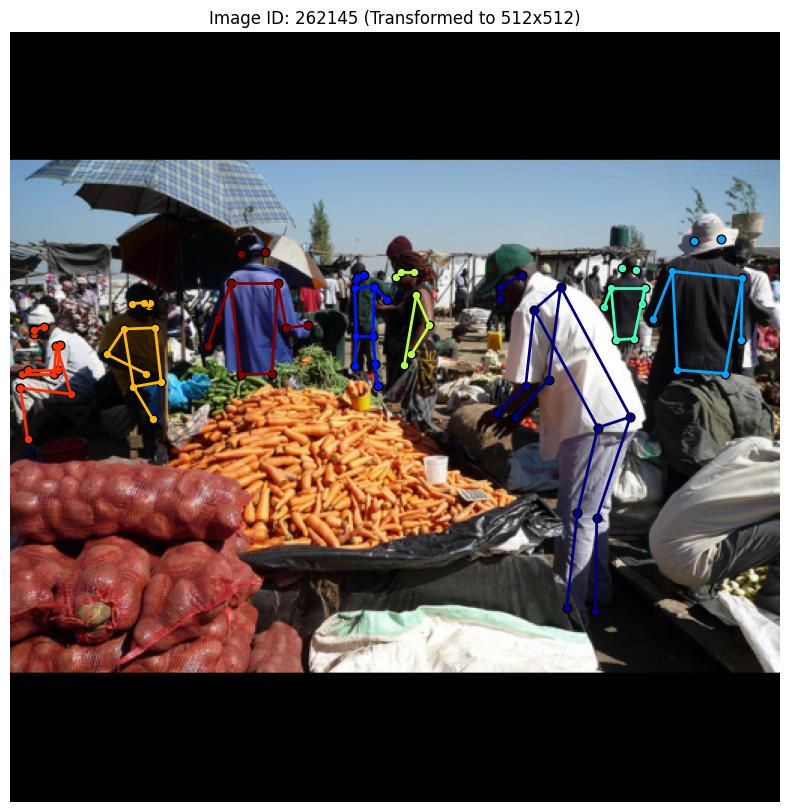
\includegraphics[width=0.4\linewidth]{figures/vis_transformed_262145.jpg}
	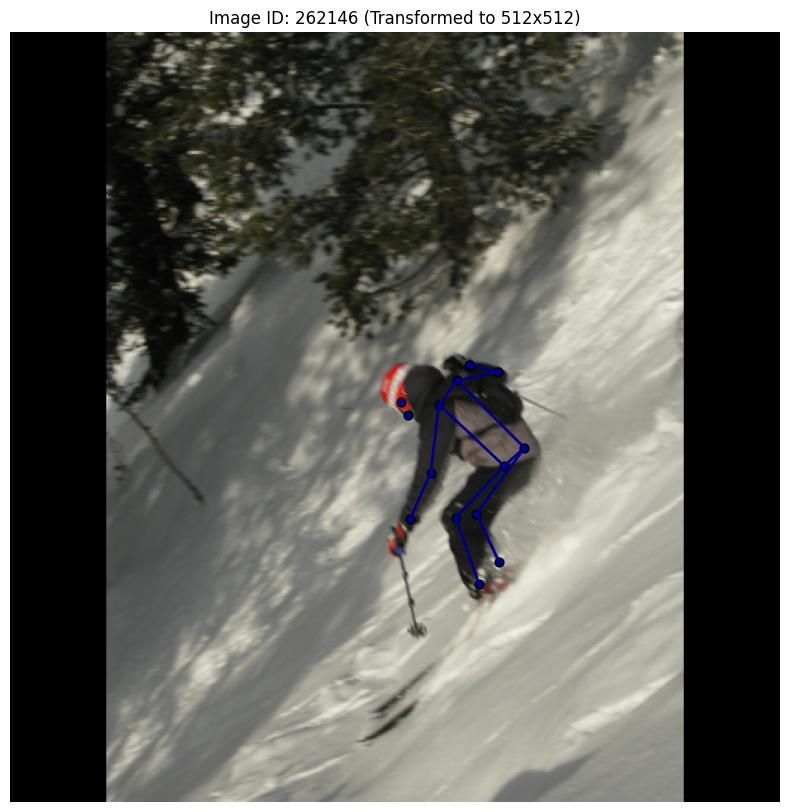
\includegraphics[width=0.4\linewidth]{figures/vis_transformed_262146.jpg}
	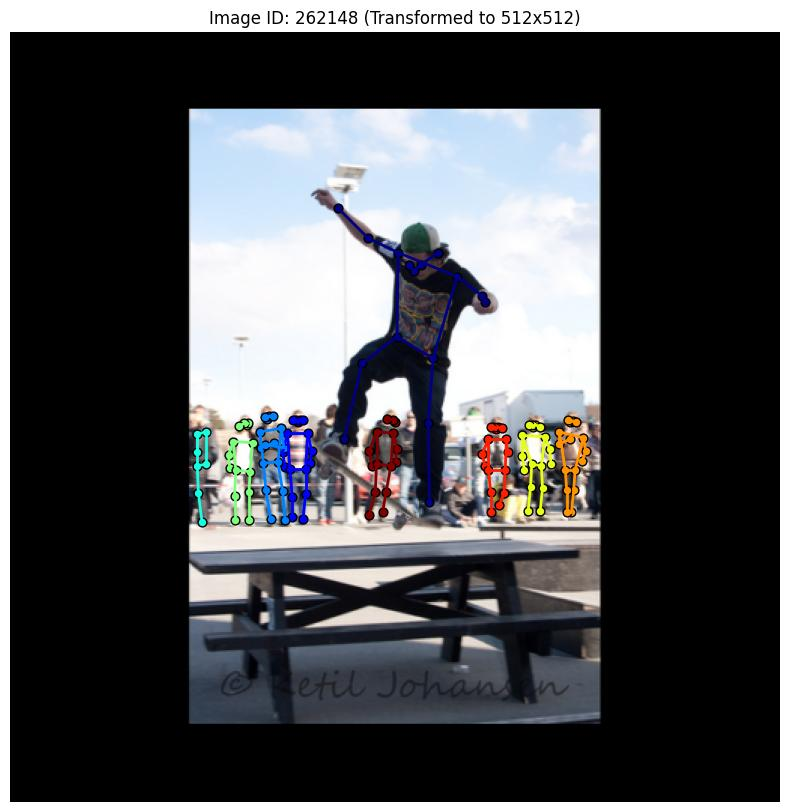
\includegraphics[width=0.4\linewidth]{figures/vis_transformed_262148.jpg}
	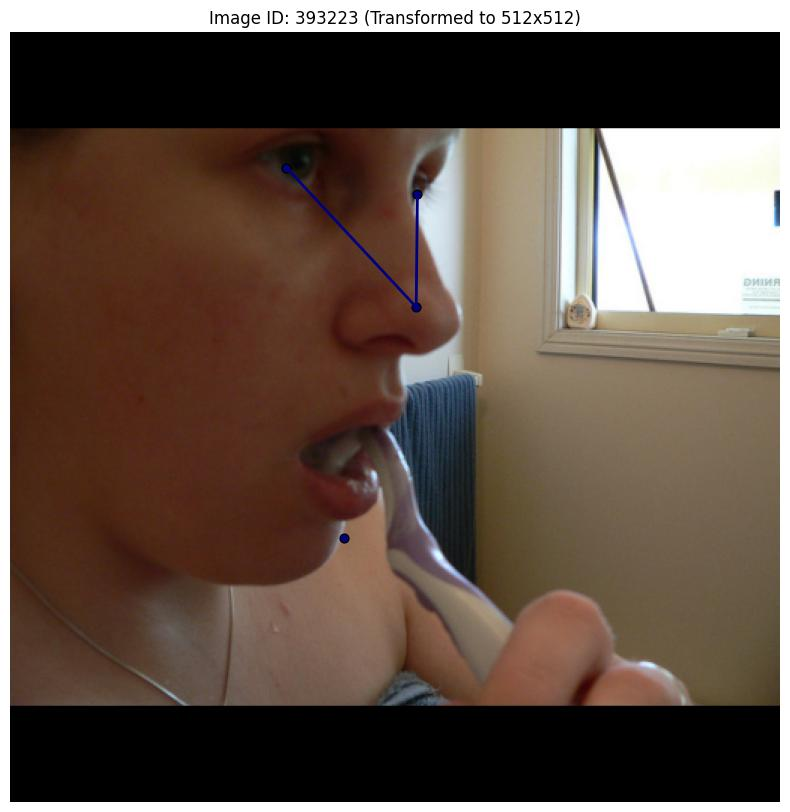
\includegraphics[width=0.4\linewidth]{figures/vis_transformed_393223.jpg}
	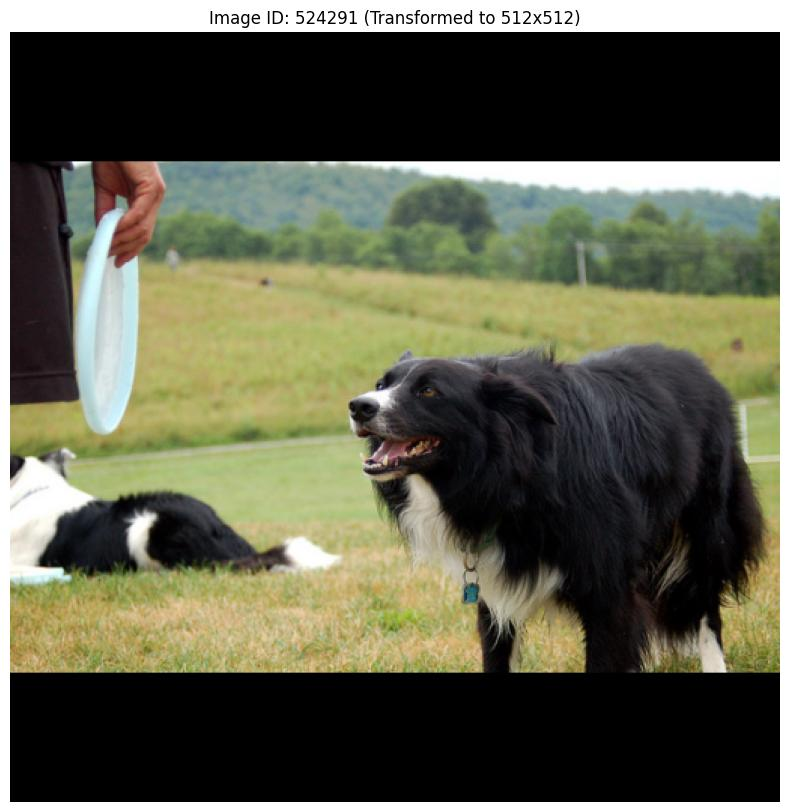
\includegraphics[width=0.4\linewidth]{figures/vis_transformed_524291.jpg}
	\caption{Example images after transformation. The images are scaled to 512x512 pixels and the keypoints are transformed accordingly.}
	\label{fig:scaled_and_padded_images}
\end{figure}

Looking at these images they look correct (mostly will touch on the one images) in the following ways:

\begin{compactitem}
	\item The images are all 512x512 pixels
	\item The keypoints are scaled correctly
	\item The padding is applied
	\item The keypoints are visible on the images
\end{compactitem}

Now I'm not 100\% sure what has happened with the $5^{th}$ image of the dog. The scaling looks correct but there are no human keypoints
but there is a human hand in the image. I'll have to deal with this later there are a number of images that are like this actually
after going through a number of the images manually but the scaling seems to work quite well

\todoredefined{Investigate why some images have no keypoints}

\begin{lstlisting}[style=pythonstyle,title={How to visualize},label={code:dataloader_visualize}]
    batch_size = 4
    val_loader = create_coco_dataloader(
        split='val',
        batch_size=batch_size
    )

    for i in range(len(val_loader)):
        print(f"Visualizing item {i} ...")
        val_loader.dataset.visualize_item(i,save_to_file=False)
\end{lstlisting}

\subsection{Collation function}

The next step is to do a collation function. A custom collate\_fn is required
to explicity defined how to merge a list of samples from the dataset into a
single batch.

While the default collate function can handle many cases, it fails here due to
the keypoints data. The default function would successfully stack the image
tensors, as they are all pre-processed to a uniform size (e.g., 3x512x512). It
would also handle img\_id and ann\_ids by collecting them into lists.

The problem arises with keypoints. The \_\_getitem\_\_ method returns a list of
keypoint tensors for each image, and the length of this list varies depending
on the number of people in the image. The default collator attempts to stack
these lists into a single tensor, which is impossible if the lists have
different lengths.

For example, consider creating a batch of size 2, where the DataLoader fetches
samples from dataset[5] and dataset[42]. Assume here that dataset[5] has 3
people and dataset[42] has a single person. The default collate function would
attempt to stack a list of length 3 with a list of length 1, which is not
possible.

\begin{compactitem}
	\item images will be stacked into a single tensor of shape $[batch\_size, 3, 512, 512]$ so in this case $[2, 3, 512, 512]$
	\item img\_ids and ann\_ids will be collected into lists of length
	\item The keypoints will be collected into a list of lists [[tensor\_p1\_img\_1,tensor\_p2\_img\_1,tensor\_p3\_img\_1],[tensor\_p1\_img\_2]]
\end{compactitem}

The coco\_collate\_fn defines a specific rule for the keypoints.
Instead of trying to stack the tensors, it gathers the individual lists into a
single list of lists. For the example above, the keypoints component of the
final batch would be [[tensor\_p1\_img\_1,tensor\_p2\_img\_1,tensor\_p3\_img\_1],[tensor\_p1\_img\_2]]. This
is a valid structure that preserves the variable number of instances per image
and prevents the program from crashing, allowing the batch to be passed to the
model for processing.


\begin{lstlisting}[style=pythonstyle,title={Custom collation function},label={code:dataloader_collate_fn}]
def coco_collate_fn(batch: List[Dict[str, Any]]) -> Dict[str, Any]:
    """
    Custom collate function to handle batches with a variable number of persons.
    """

    # Stack images, which are all the same size
    images = torch.stack([item['image'] for item in batch], dim=0)

    # For keypoints, can't stack them directly.
    # Keep them as a list of lists of tensors.
    # The outer list represents the batch, the inner list is the people in an image.
    keypoints = [item['keypoints'] for item in batch]
    
    # Other metadata can be collected into lists
    img_ids = [item['img_id'] for item in batch]
    ann_ids = [item['ann_ids'] for item in batch]

    return {
        'image': images,
        'keypoints': keypoints,
        'img_id': img_ids,
        'ann_ids': ann_ids
    }
\end{lstlisting}

\section[2025/06/20]{Friday, 20 June 2025}
\label{sec:20250620}

The task is to get this working and training.

I've had to do a number of things in order to get this working.

One issue was with the depth estimator. The initial implementation of the
\texttt{estimate\_depth} function loaded the pre-trained MiDaS model
every time the function was called which happened for each image during preprocessing.
This was fixed by moving the model loading into the \texttt{KeypointPreprocessor}
class so it only happened once. \texttt{estimate\_depth} was then refactored
to accept the preloaded model

Then I needed to update the \texttt{KeypointPreprocessor} and \texttt{GAT}
to work with PyTorch Geometric (PyG)

The \texttt{KeypointPreprocessor} also required a rework to align with PyTorch
Geometric (PyG). The original preprocessor was designed to output a list of
Python dictionaries containing dense adjacency matrices. This format is
memory-intensive and incompatible with the PyG \texttt{DataLoader} and GNN
layers, which expect graph data to be encapsulated in a
\texttt{torch\_geometric.data.Data} object. The fix involved modifying the
preprocessor to output these \texttt{Data} objects, which required replacing
the \texttt{create\_adjacency\_matrix} method with a more efficient
\texttt{create\_edge\_index} function. This new function generates graph
connectivity in the sparse Coordinate (COO) format (\texttt{[2, num\_edges]}),
which is the standard for PyG.

The \texttt{DepthAwareGAT} model itself was refactored to align with the PyG.
The original implementation was a "vanilla" PyTorch GAT built from scratch,
which expected a dense adjacency matrix and was incompatible with the PyG
batching object. The entire model was rewritten using PyG's native
\texttt{GATConv} layer. This new layer is highly optimized, handles multi-head
attention internally, and is designed to work directly with the sparse
\texttt{edge\_index} format. The model's \texttt{forward} method signature was
also updated to accept the standard PyG \texttt{Batch} object attributes
(\texttt{x}, \texttt{edge\_index}, \texttt{batch})


The \texttt{BasicGATTrainer} class was refined (not changed too much) to ensure all trainable
components of the pipeline were correctly optimized. The primary issue was that
the \texttt{KeypointPreprocessor} contains a learnable \texttt{nn.Embedding}
layer for joint types. Initially, the optimizer in the trainer was only
configured to update the parameters of the \texttt{DepthAwareGAT} model,
leaving the embeddings untrained. To rectify this, the
\texttt{BasicGATTrainer}'s constructor was updated to accept the
\texttt{KeypointPreprocessor} instance, and its parameters were explicitly
included in the optimizer's parameter list. Additionally, a crucial robustness
improvement was made within the \texttt{KeypointPreprocessor}'s
\texttt{extract\_node\_features} method: the generated node features are now
explicitly \texttt{detach()}-ed from their computation graph before being
stored in the \texttt{torch\_geometric.data.Data} objects. This prevents a
"backward through graph a second time" runtime error during subsequent training
epochs, as it ensures that the data fed to the model in each epoch is treated
as fresh input without retaining stale computational history.

\subsection{Training test}

Running the training on the "val" test as a first order test (the training set is much larger)

The following parameters were used:

\begin{lstlisting}[style=pythonstyle,title={First training test},label={code:first_training_test}]
batch_size_raw_data = 16
batch_size_trainer = 8
learning_rate = 0.001
num_epochs = 100
\end{lstlisting}

for simplicity sake the main file is given

\begin{lstlisting}[style=pythonstyle,title={Basic training main for recreation later},label={code:basic_training_main}]
def main():
    device = torch.device('cuda' if torch.cuda.is_available() else 'cpu')
    print(f"Using device: {device}")

    batch_size_raw_data = 16
    batch_size_trainer = 8
    learning_rate = 0.001
    num_epochs = 100
    
    embedding_dim = 32
    keypoint_preprocessor = KeypointPreprocessor(embedding_dim=embedding_dim, device=device)
    
    print("\n--- Starting Data Preprocessing (this might take a while) ---")
    train_loader_raw = create_coco_dataloader(
        split='val',
        batch_size=batch_size_raw_data,
        shuffle=False,
        num_workers=4
    )
    
    processed_train_graphs = []
    for i, batch in enumerate(train_loader_raw):
        pyg_graphs = keypoint_preprocessor.process_batch(batch)
        processed_train_graphs.extend(pyg_graphs)
        if (i + 1) % 100 == 0:
            print(f"Processed {i + 1} raw batches, total graphs: {len(processed_train_graphs)}")

    print(f"\nFinished preprocessing. Total training graphs: {len(processed_train_graphs)}")
    
    print("\nAnalyzing processed dataset statistics...")
    analyze_dataset(processed_train_graphs)

    gat_model = DepthAwareGAT(
        input_dim=4 + embedding_dim,
        hidden_dim=64,
        output_dim=32,
        num_heads=4,
        dropout=0.6
    )

    trainer = BasicGATTrainer(model=gat_model,preprocessor=keypoint_preprocessor, output_dir=settings.output_dir)

    print("\n--- Starting GAT Training ---")
    trained_model = trainer.train(
        dataset=processed_train_graphs,
        epochs=num_epochs,
        batch_size=batch_size_trainer,
        lr=learning_rate
    )
    print("\nTraining process completed.")
\end{lstlisting}

this gives the details

\begin{figure}[H]
	\centering
	
\includegraphics[width=0.4\linewidth]{figures/embeddings_epoch_25.png}
	
\includegraphics[width=0.4\linewidth]{figures/embeddings_epoch_50.png}
	
\includegraphics[width=0.4\linewidth]{figures/embeddings_epoch_75.png}
	
\includegraphics[width=0.4\linewidth]{figures/embeddings_epoch_100.png}
	\caption{embeddings at different epochs}
	\label{fig:basic_embeddings_epocs}
\end{figure}

\begin{figure}[H]
	\centering
	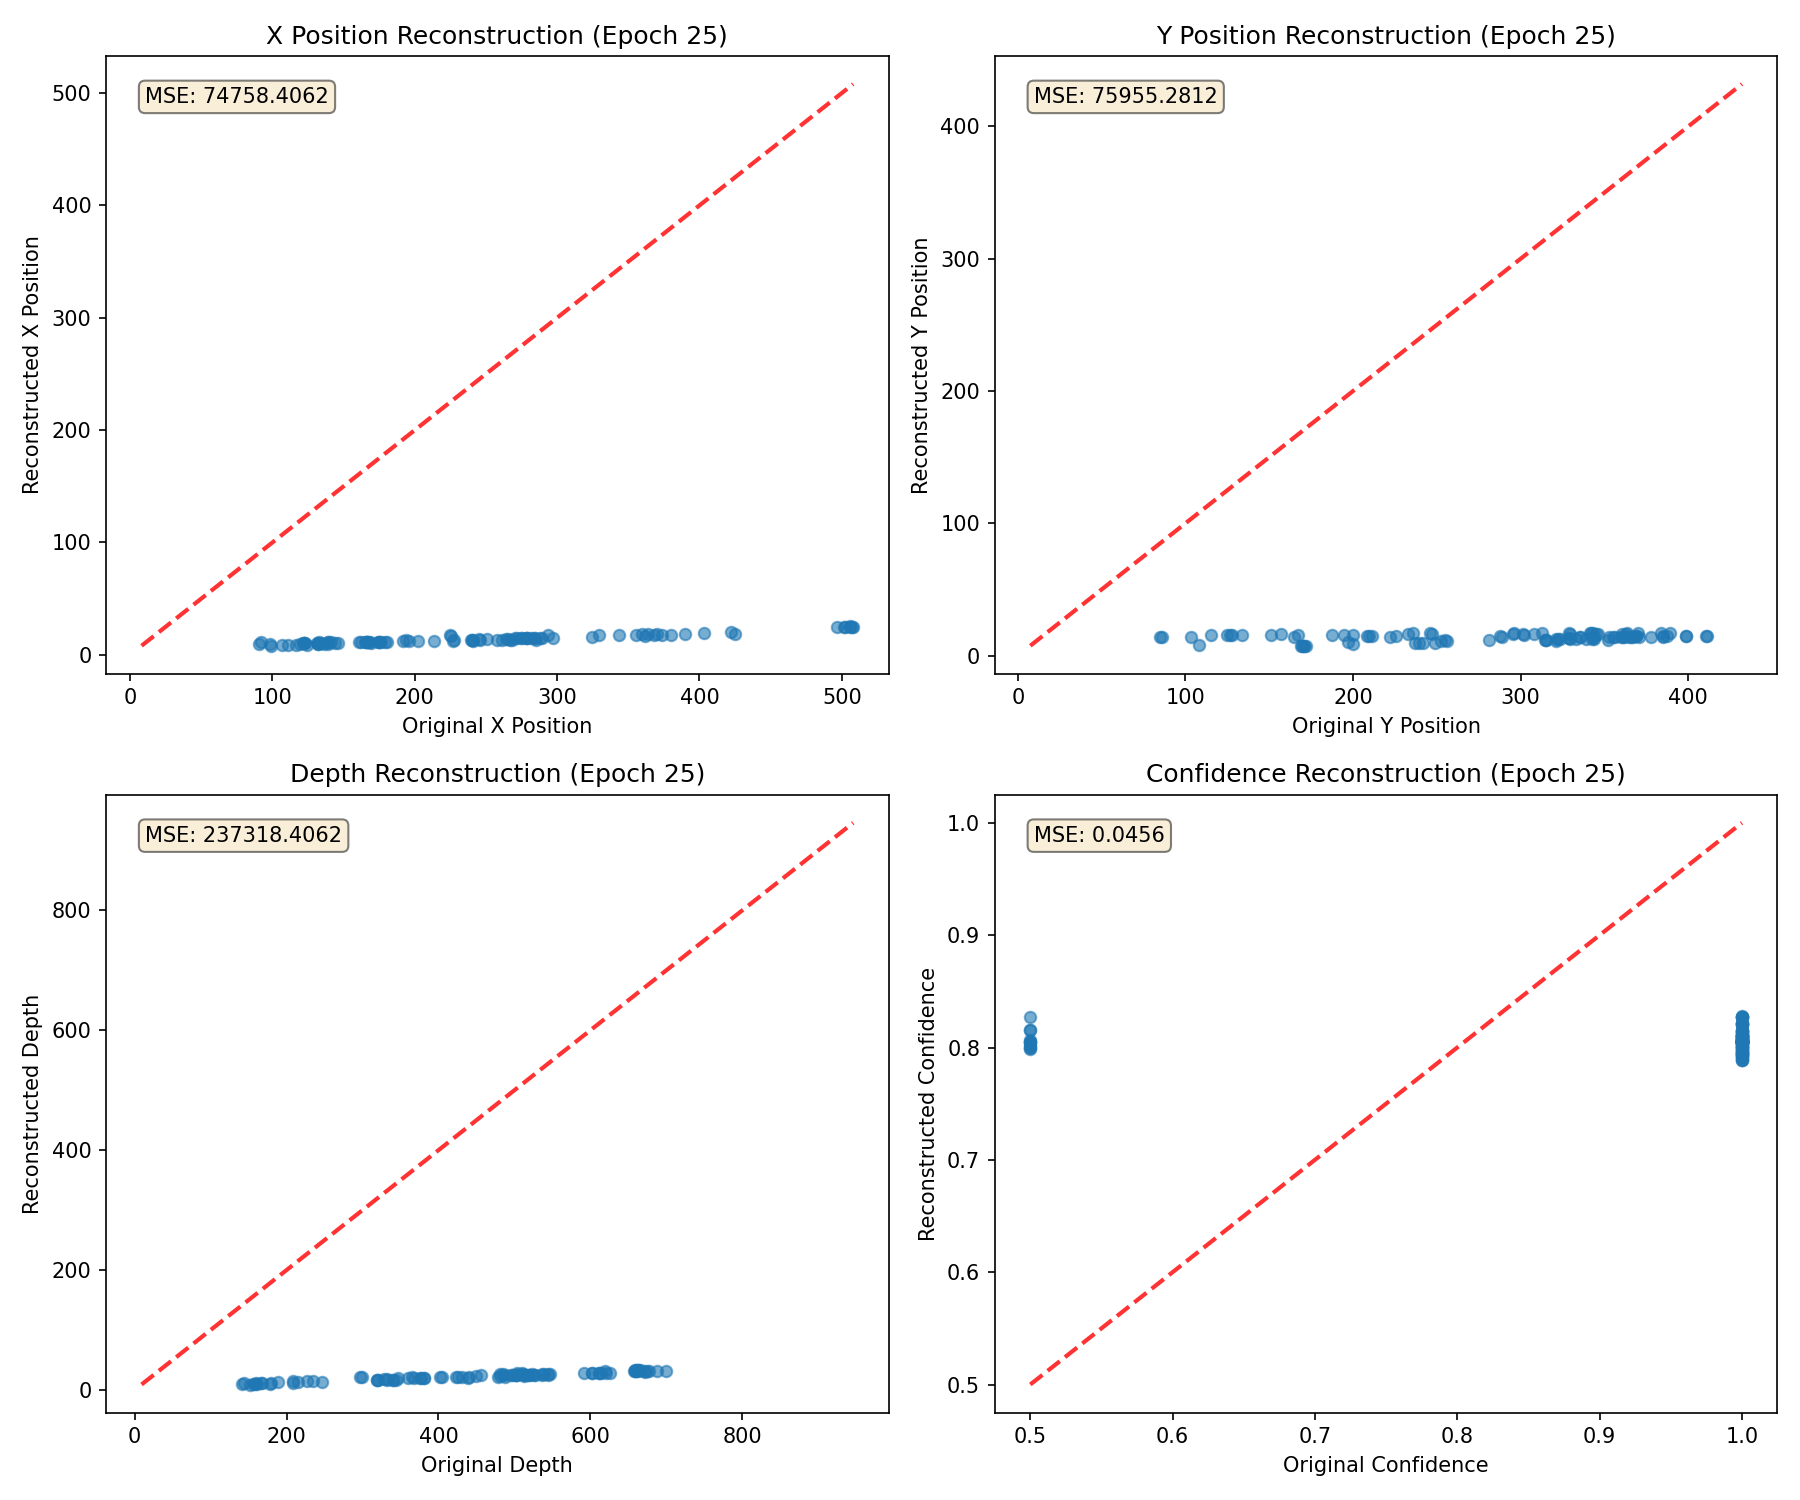
\includegraphics[width=0.4\linewidth]{figures/reconstruction_epoch_25.png}
	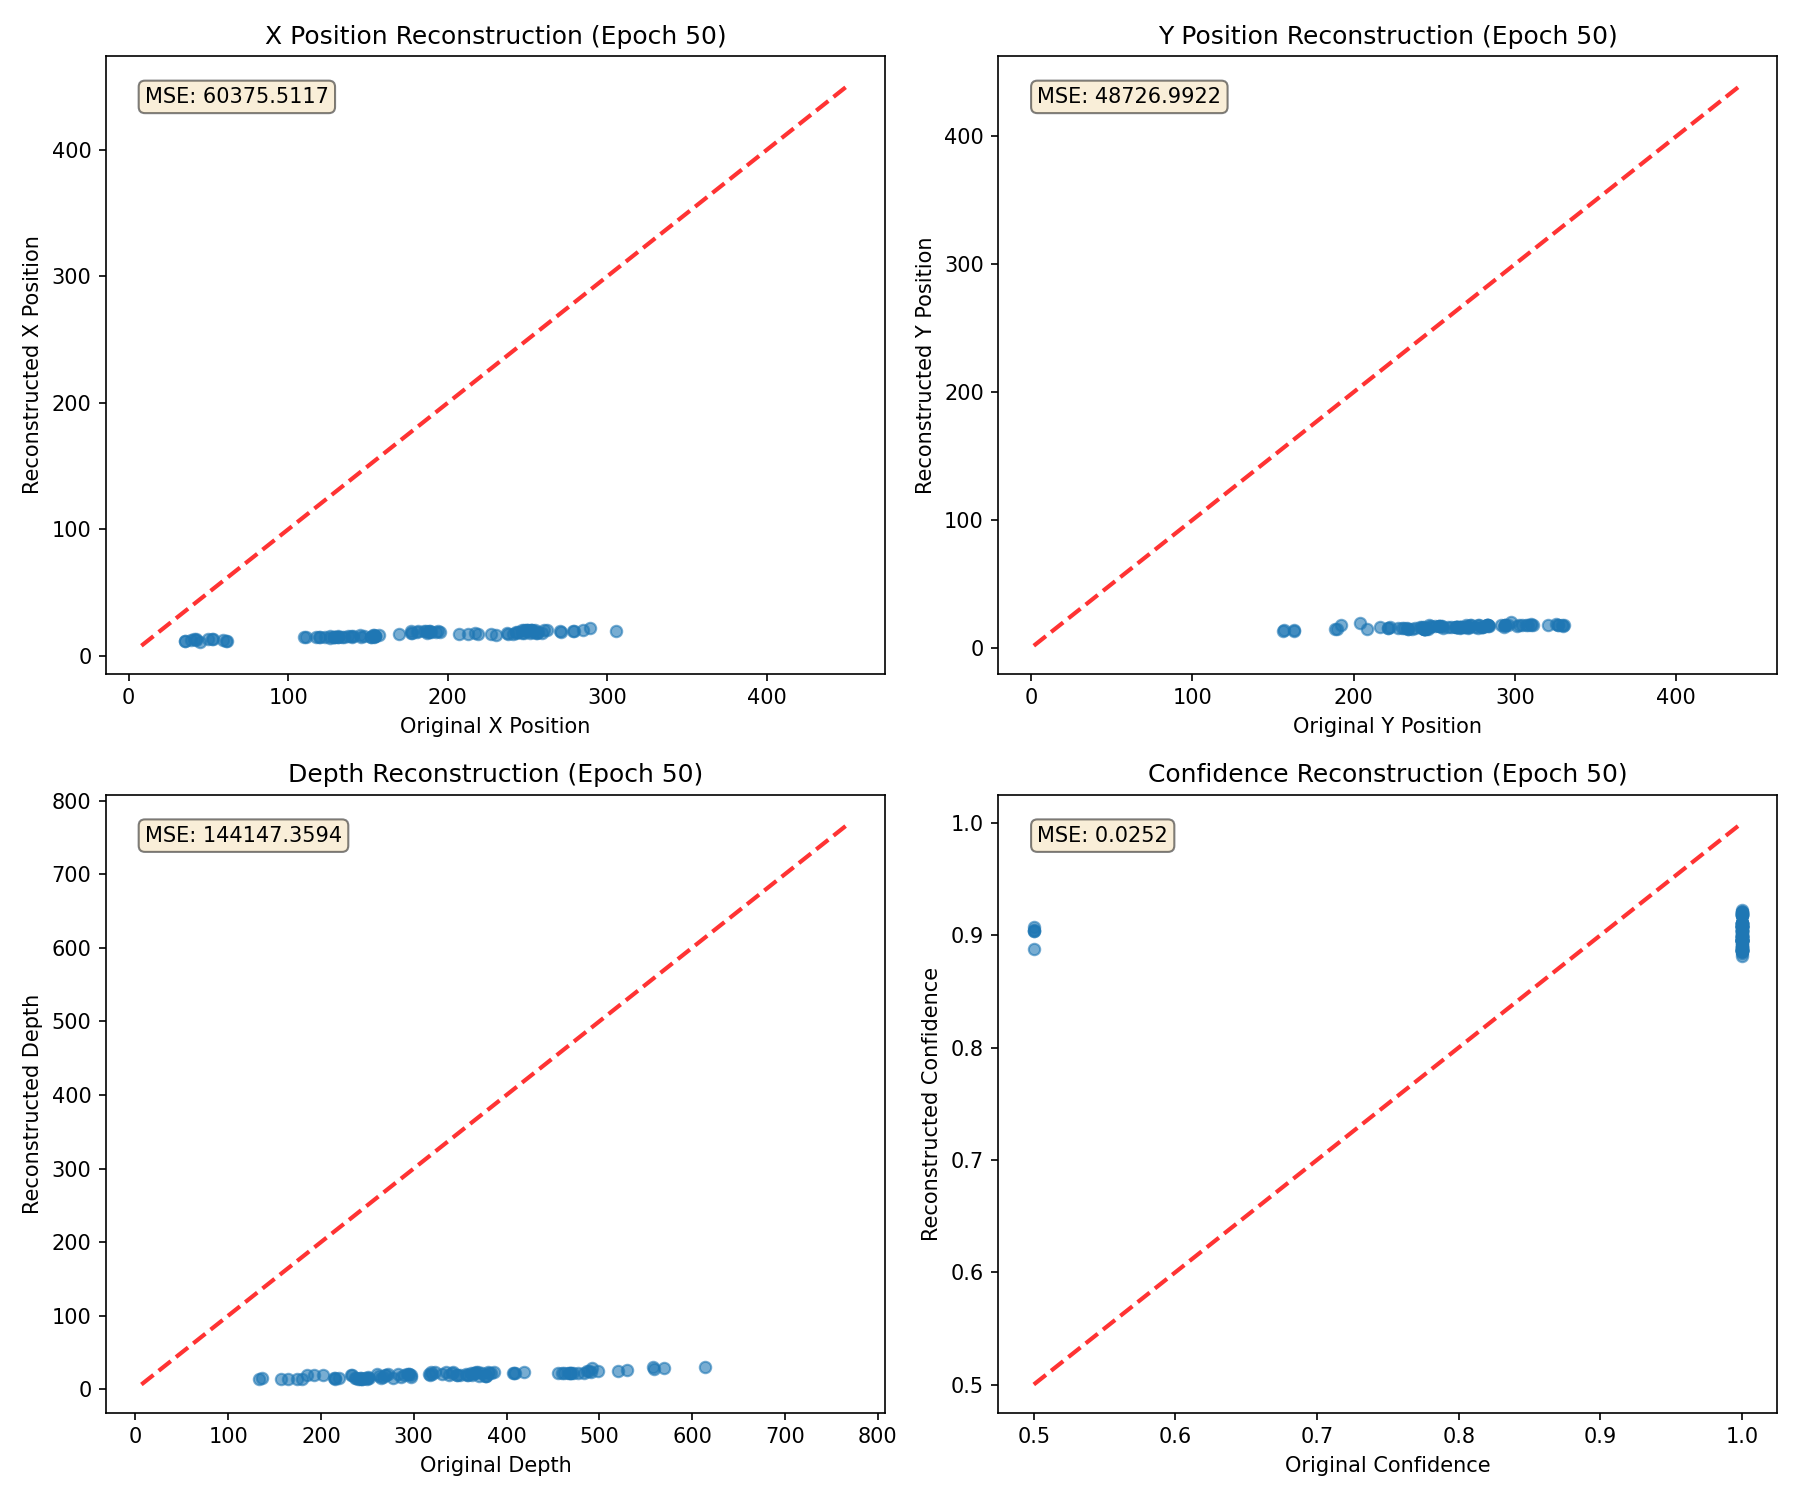
\includegraphics[width=0.4\linewidth]{figures/reconstruction_epoch_50.png}
	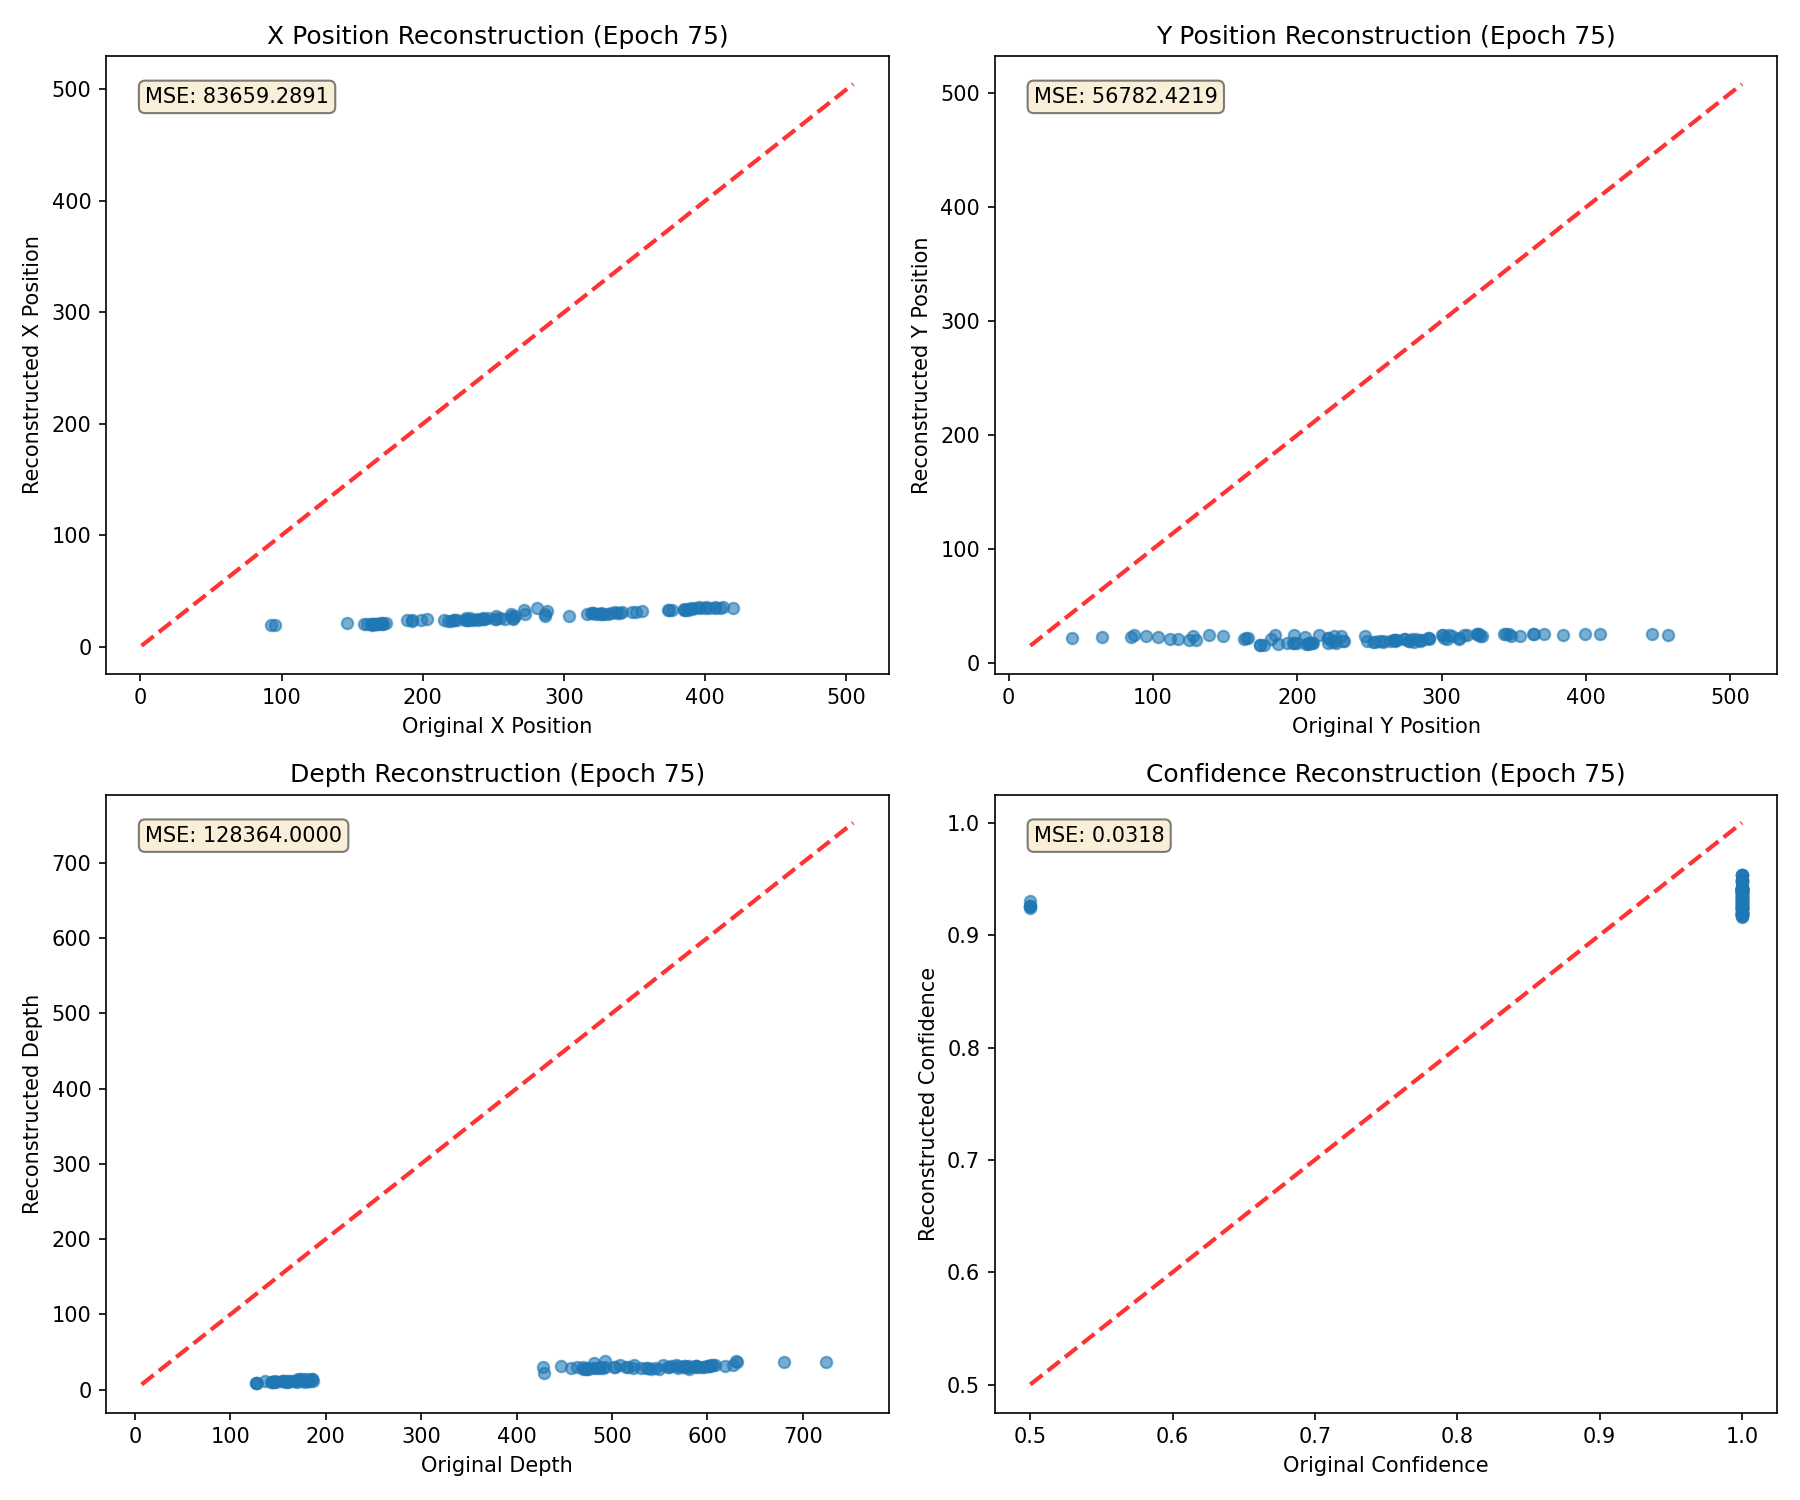
\includegraphics[width=0.4\linewidth]{figures/reconstruction_epoch_75.png}
	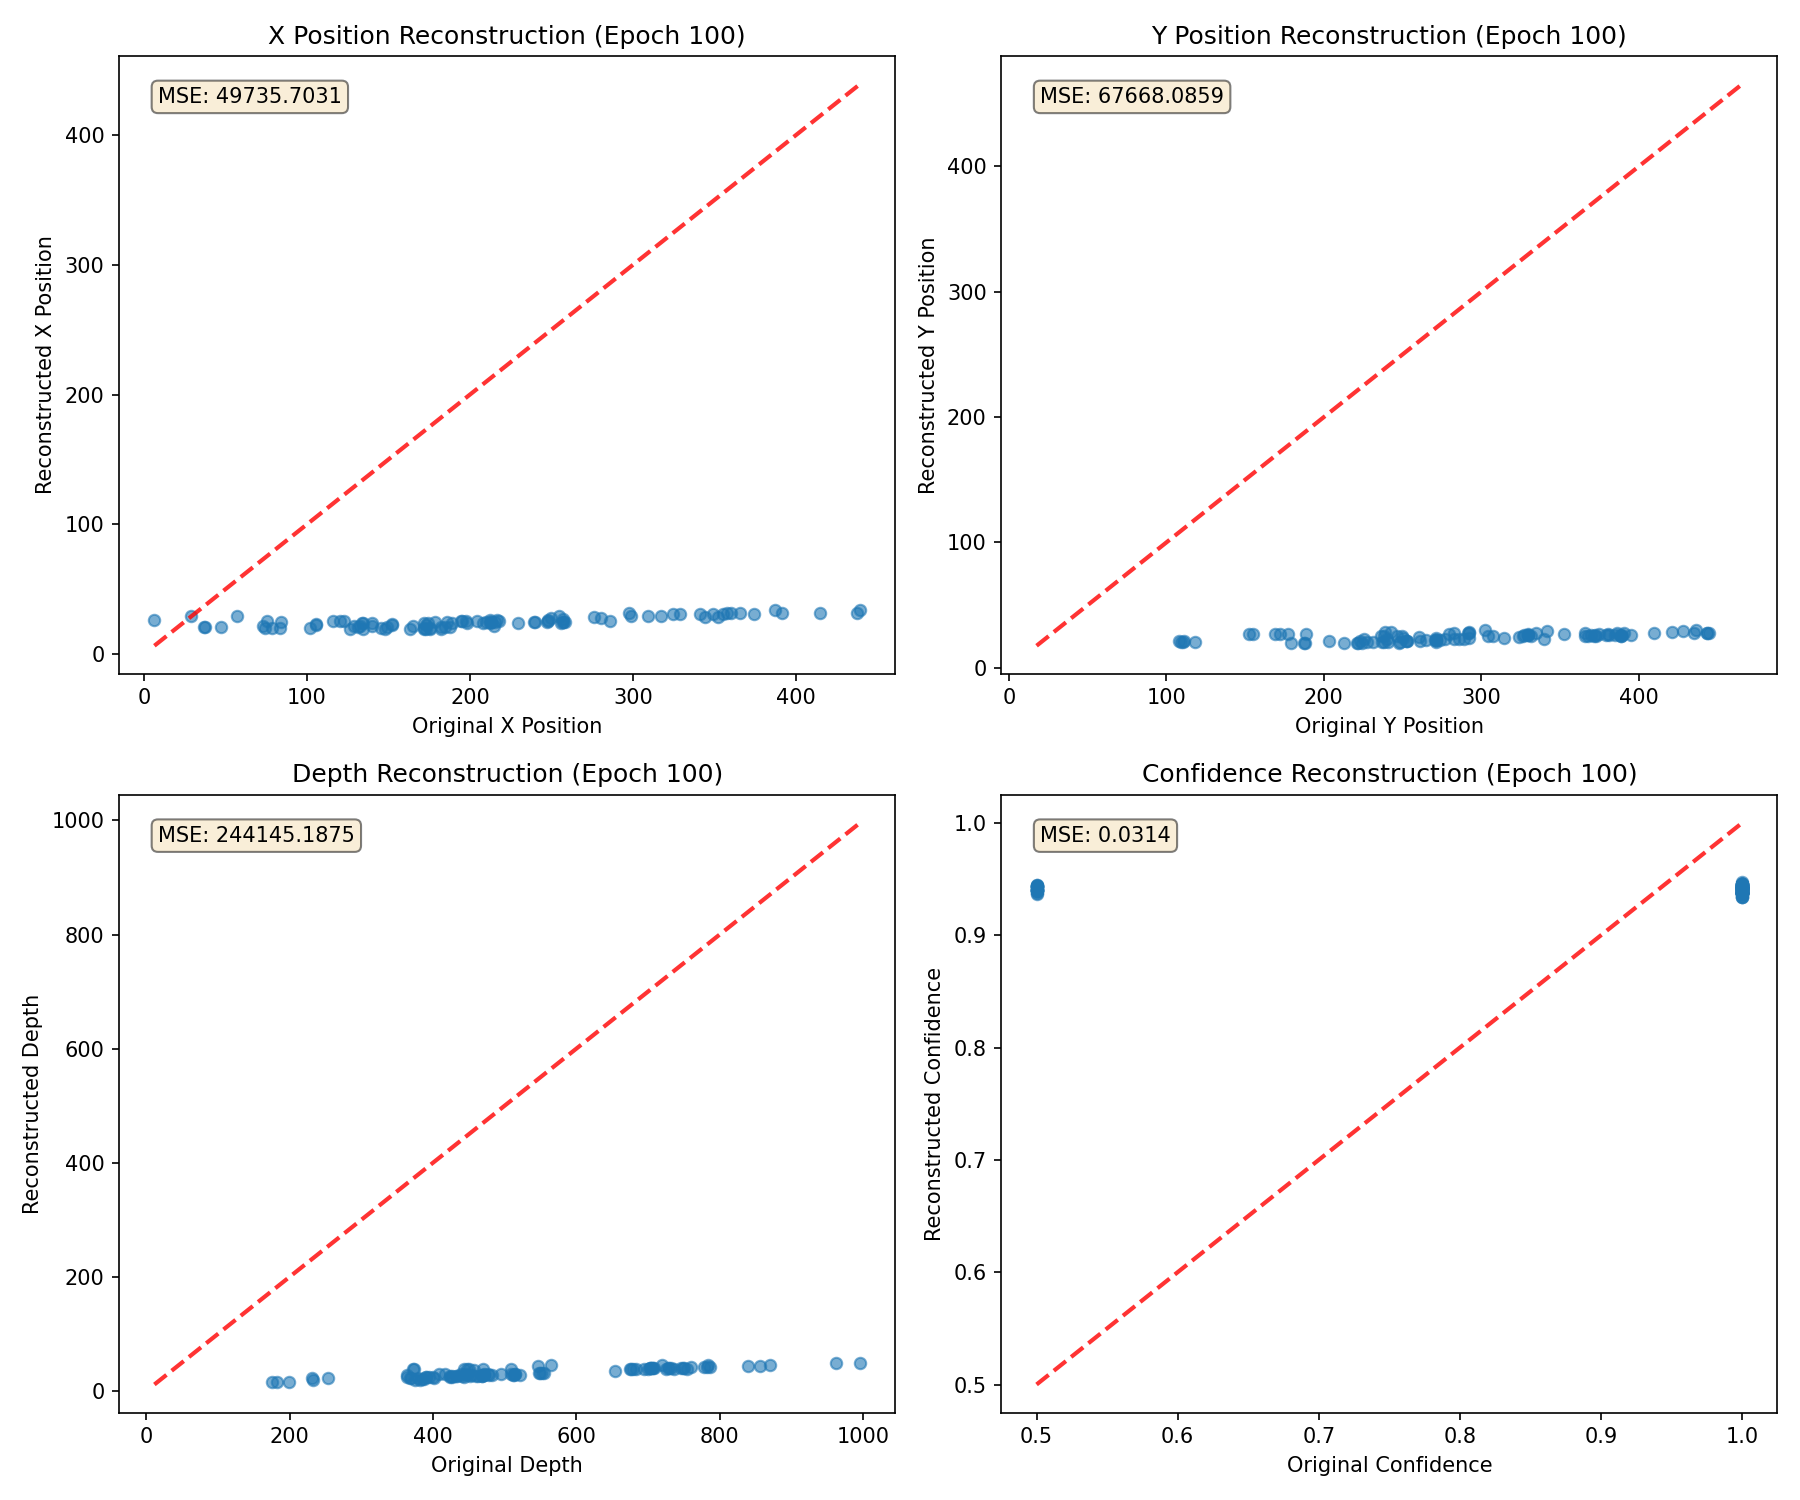
\includegraphics[width=0.4\linewidth]{figures/reconstruction_epoch_100.png}
	\caption{reconstruction at different epochs}
	\label{fig:basic_reconstruction_epocs}
\end{figure}


\begin{figure}[H]
	\centering
	
\includegraphics[width=0.4\linewidth]{figures/training_loss.png}
	\caption{Trainig loss}
	\label{fig:basic_training_loss}
\end{figure}

\section[2025/06/20]{Friday, 27 June 2025}
\label{sec:20250627}

Training first attempt with the full training set and 500 epochs

\begin{figure}[H]
	\centering
	
\includegraphics[width=0.4\linewidth]{figures/training_attempt_1/embeddings_epoch_100.png}
	
\includegraphics[width=0.4\linewidth]{figures/training_attempt_1/embeddings_epoch_200.png}
	
\includegraphics[width=0.4\linewidth]{figures/training_attempt_1/embeddings_epoch_300.png}
	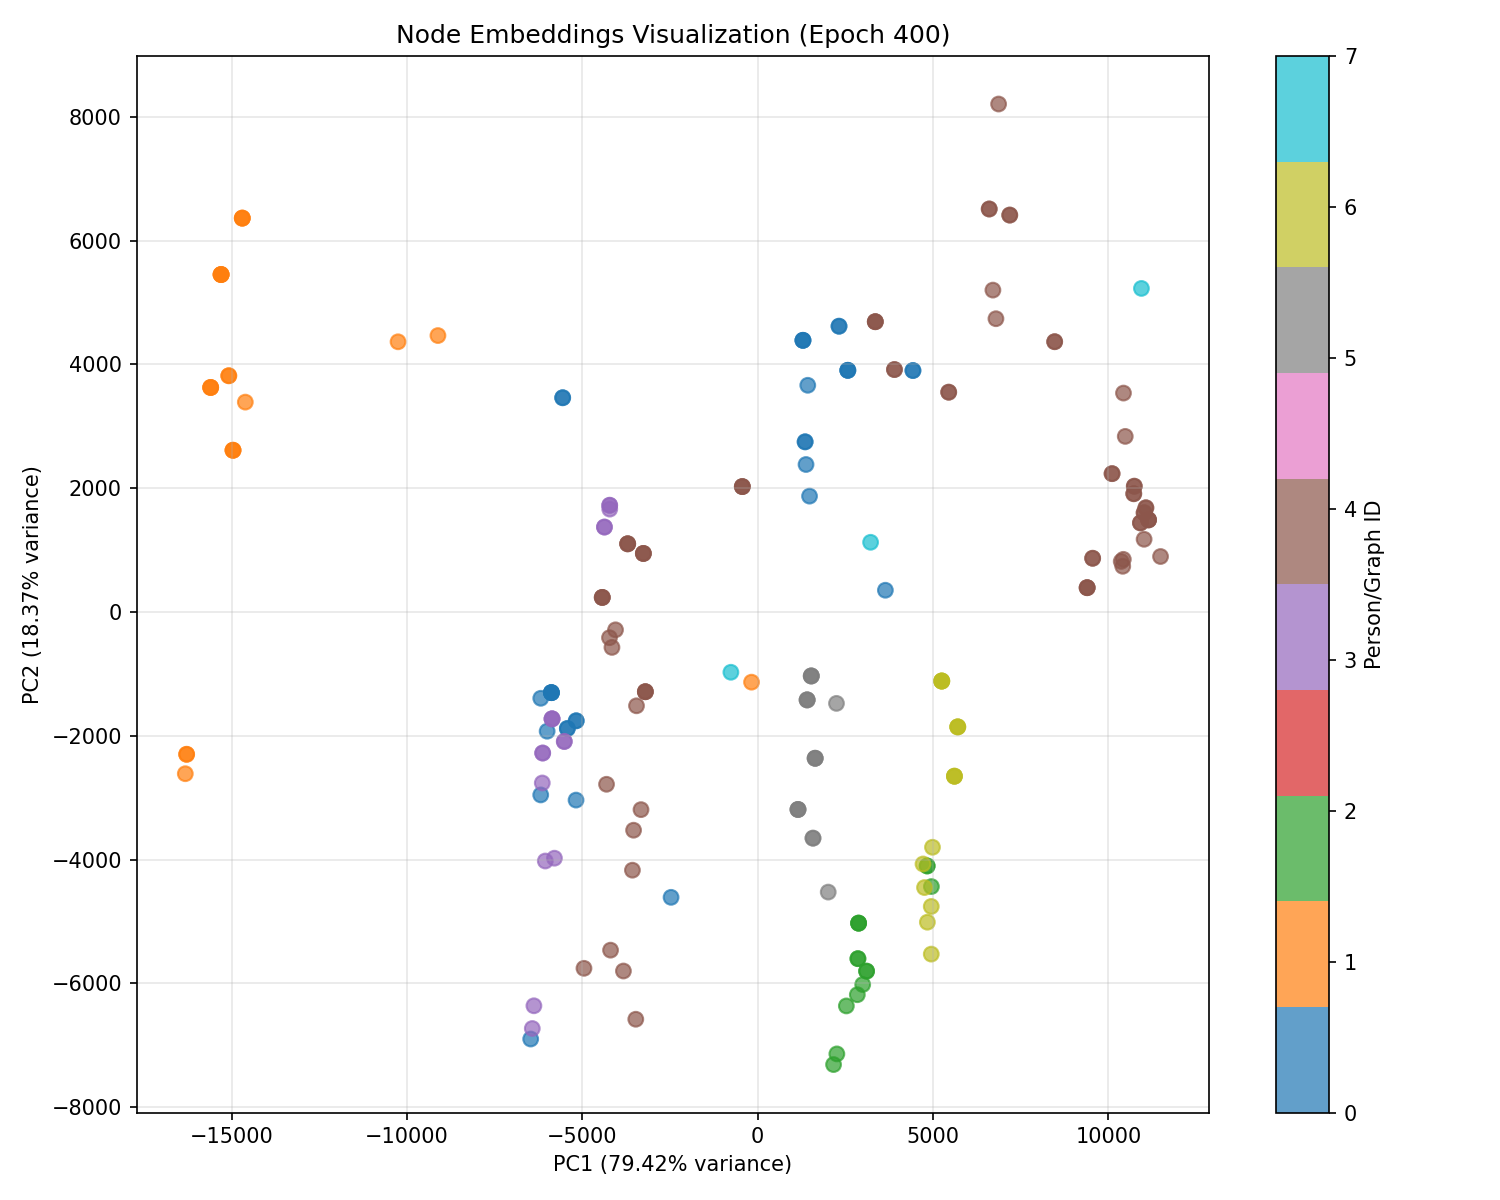
\includegraphics[width=0.4\linewidth]{figures/training_attempt_1/embeddings_epoch_400.png}
	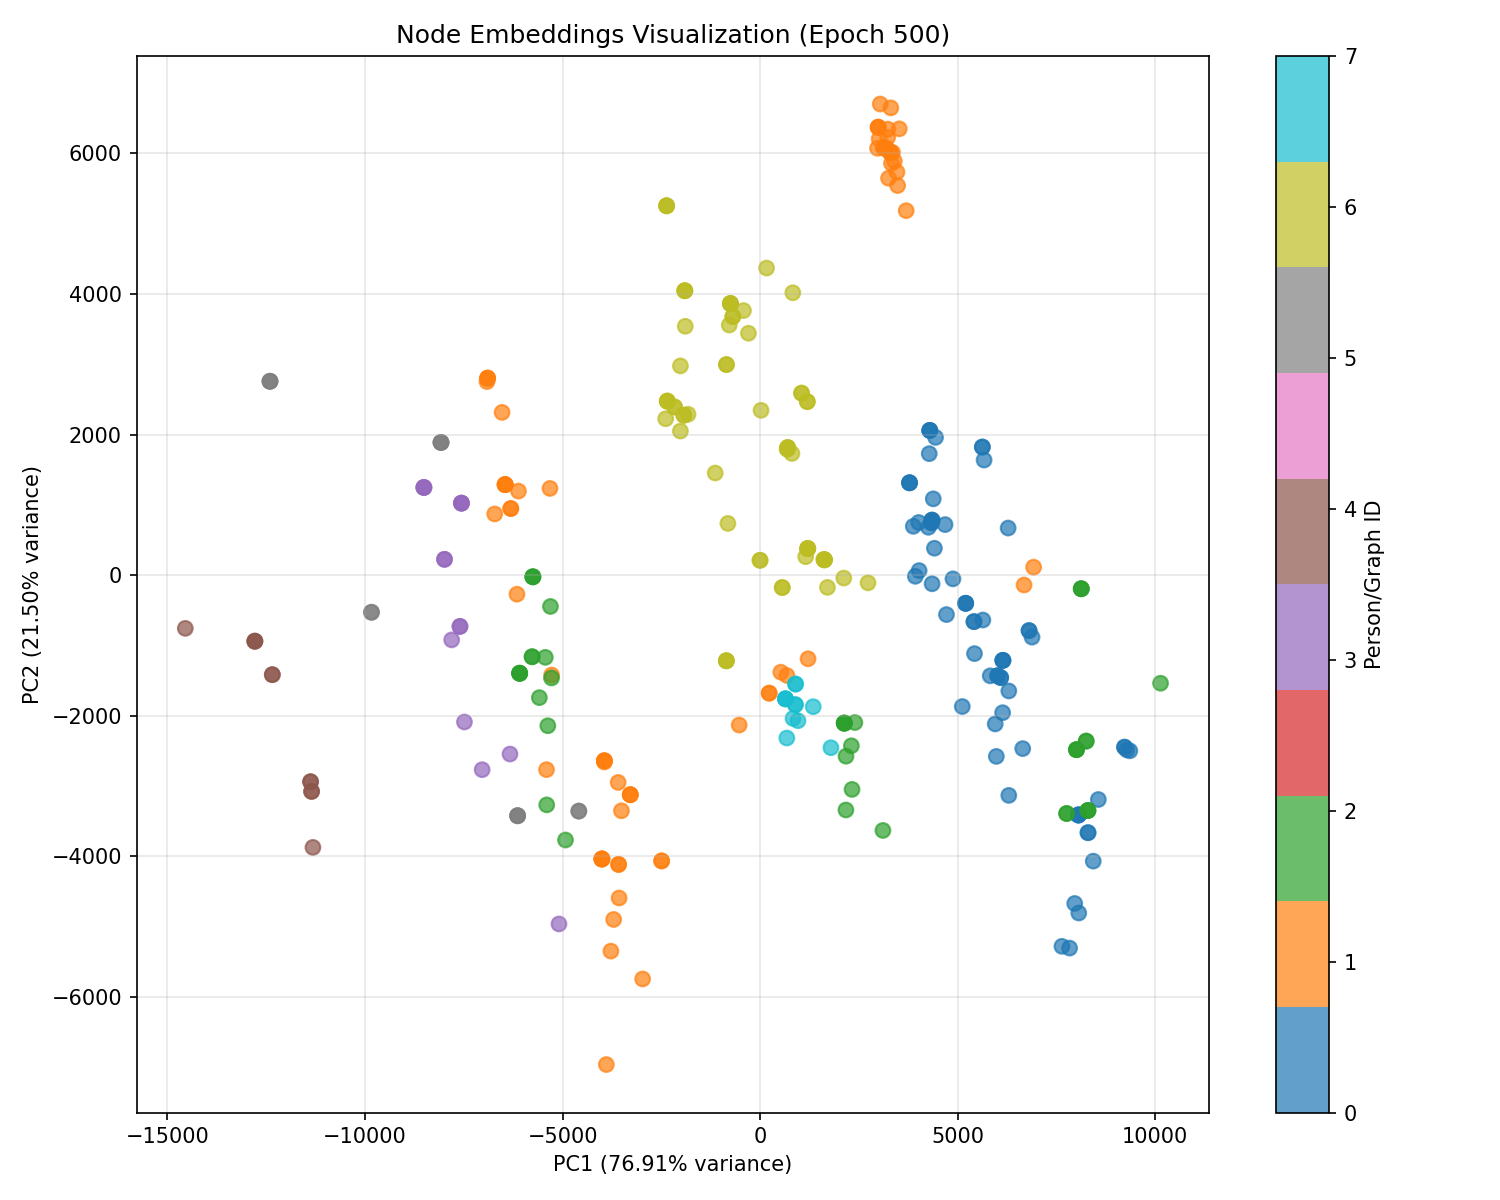
\includegraphics[width=0.4\linewidth]{figures/training_attempt_1/embeddings_epoch_500.png}
	\caption{Training with full set and 500 epochs embeddings}
	\label{fig:training_attempt_1_embeddings_epocs}
\end{figure}

\begin{figure}[H]
	\centering
	
\includegraphics[width=0.4\linewidth]{figures/training_attempt_1/reconstruction_epoch_100.png}
	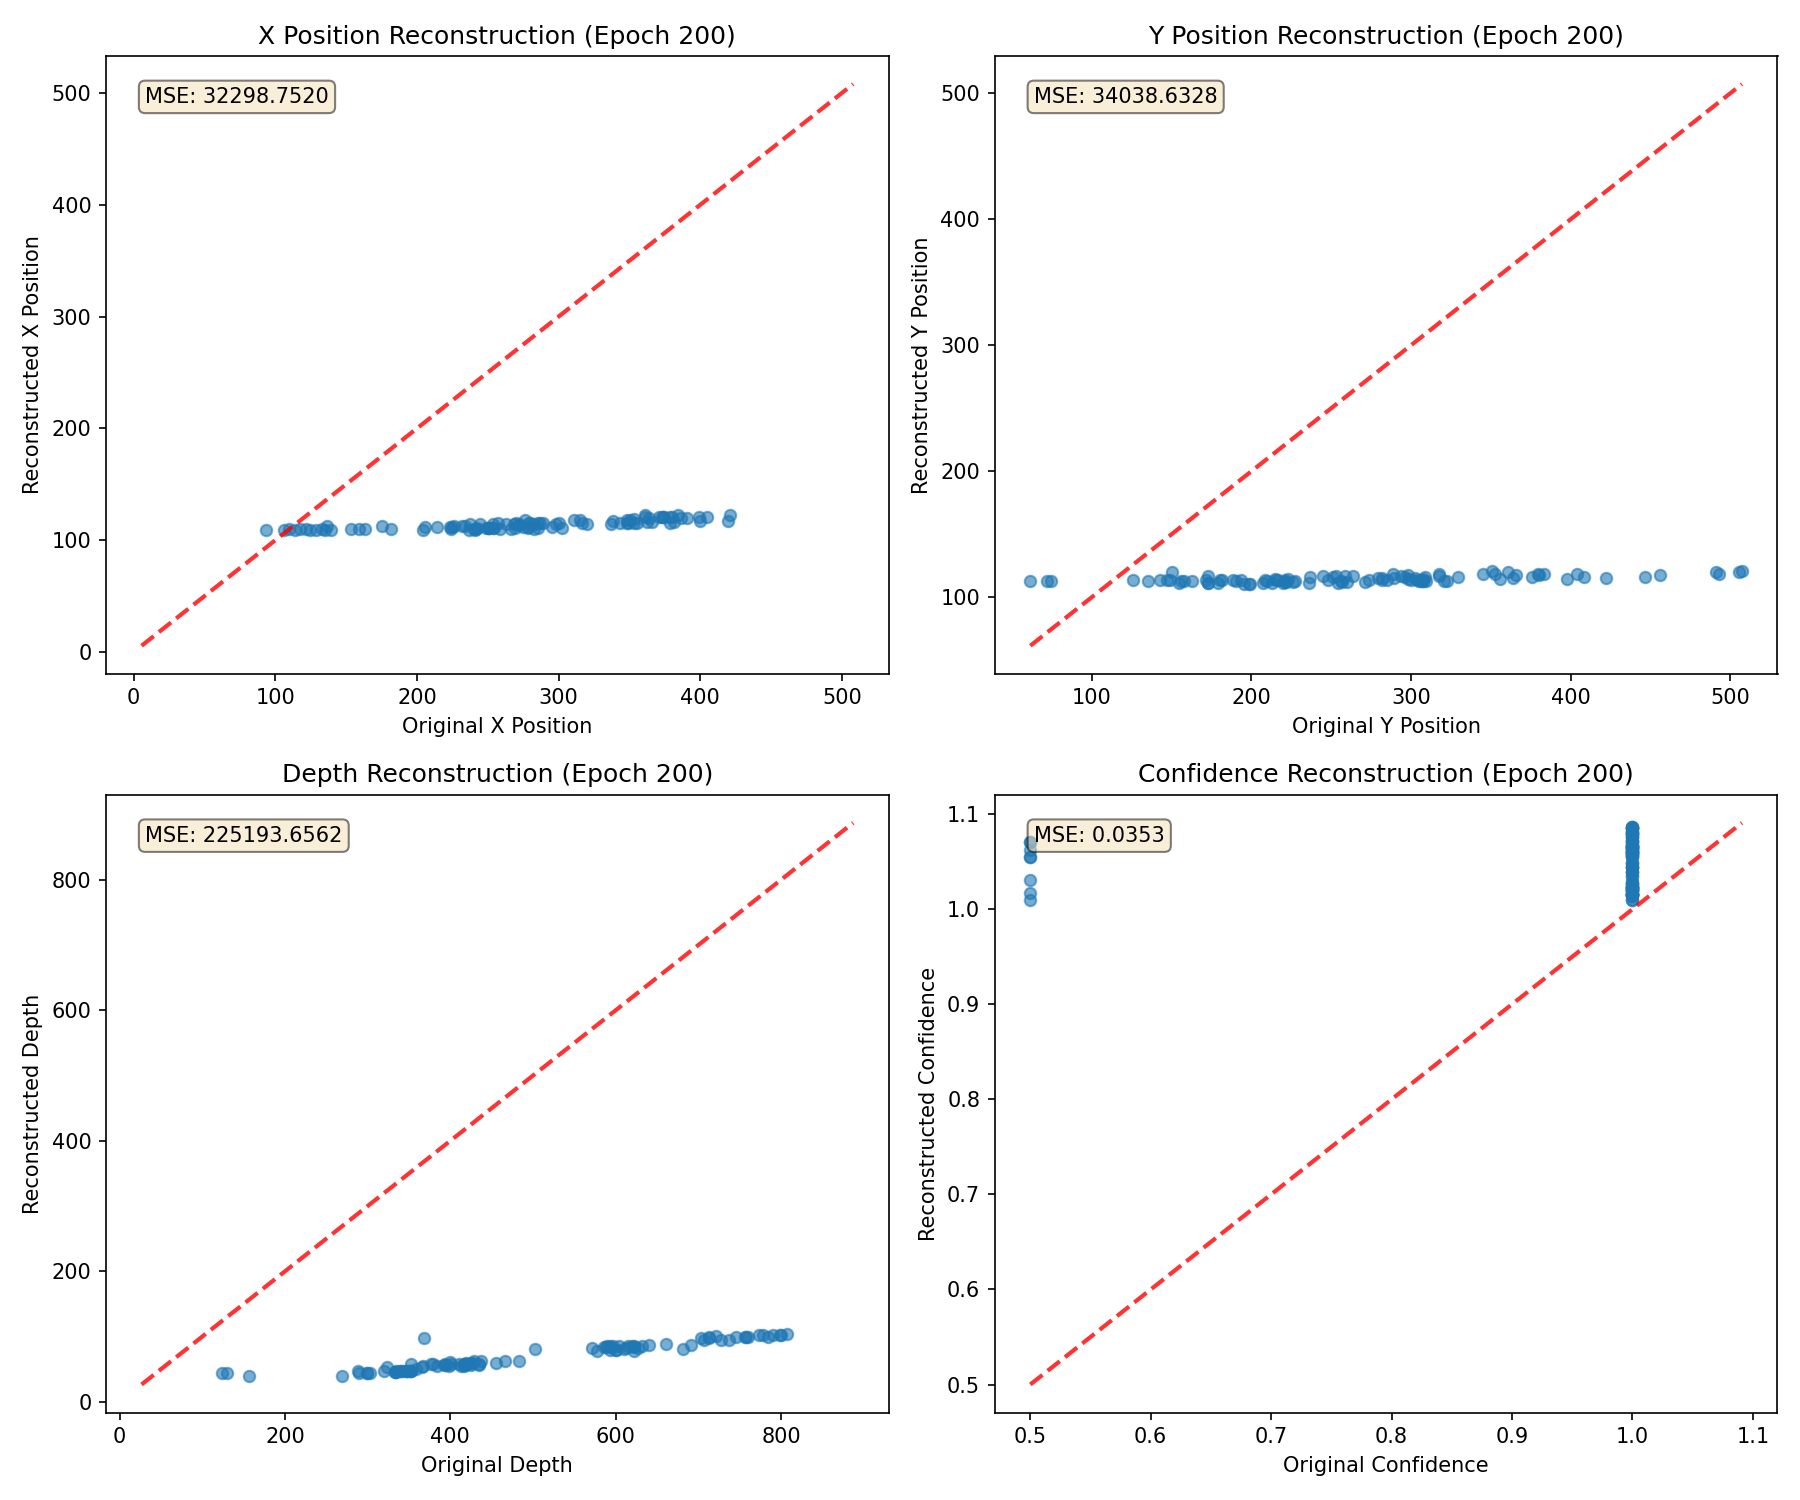
\includegraphics[width=0.4\linewidth]{figures/training_attempt_1/reconstruction_epoch_200.png}
	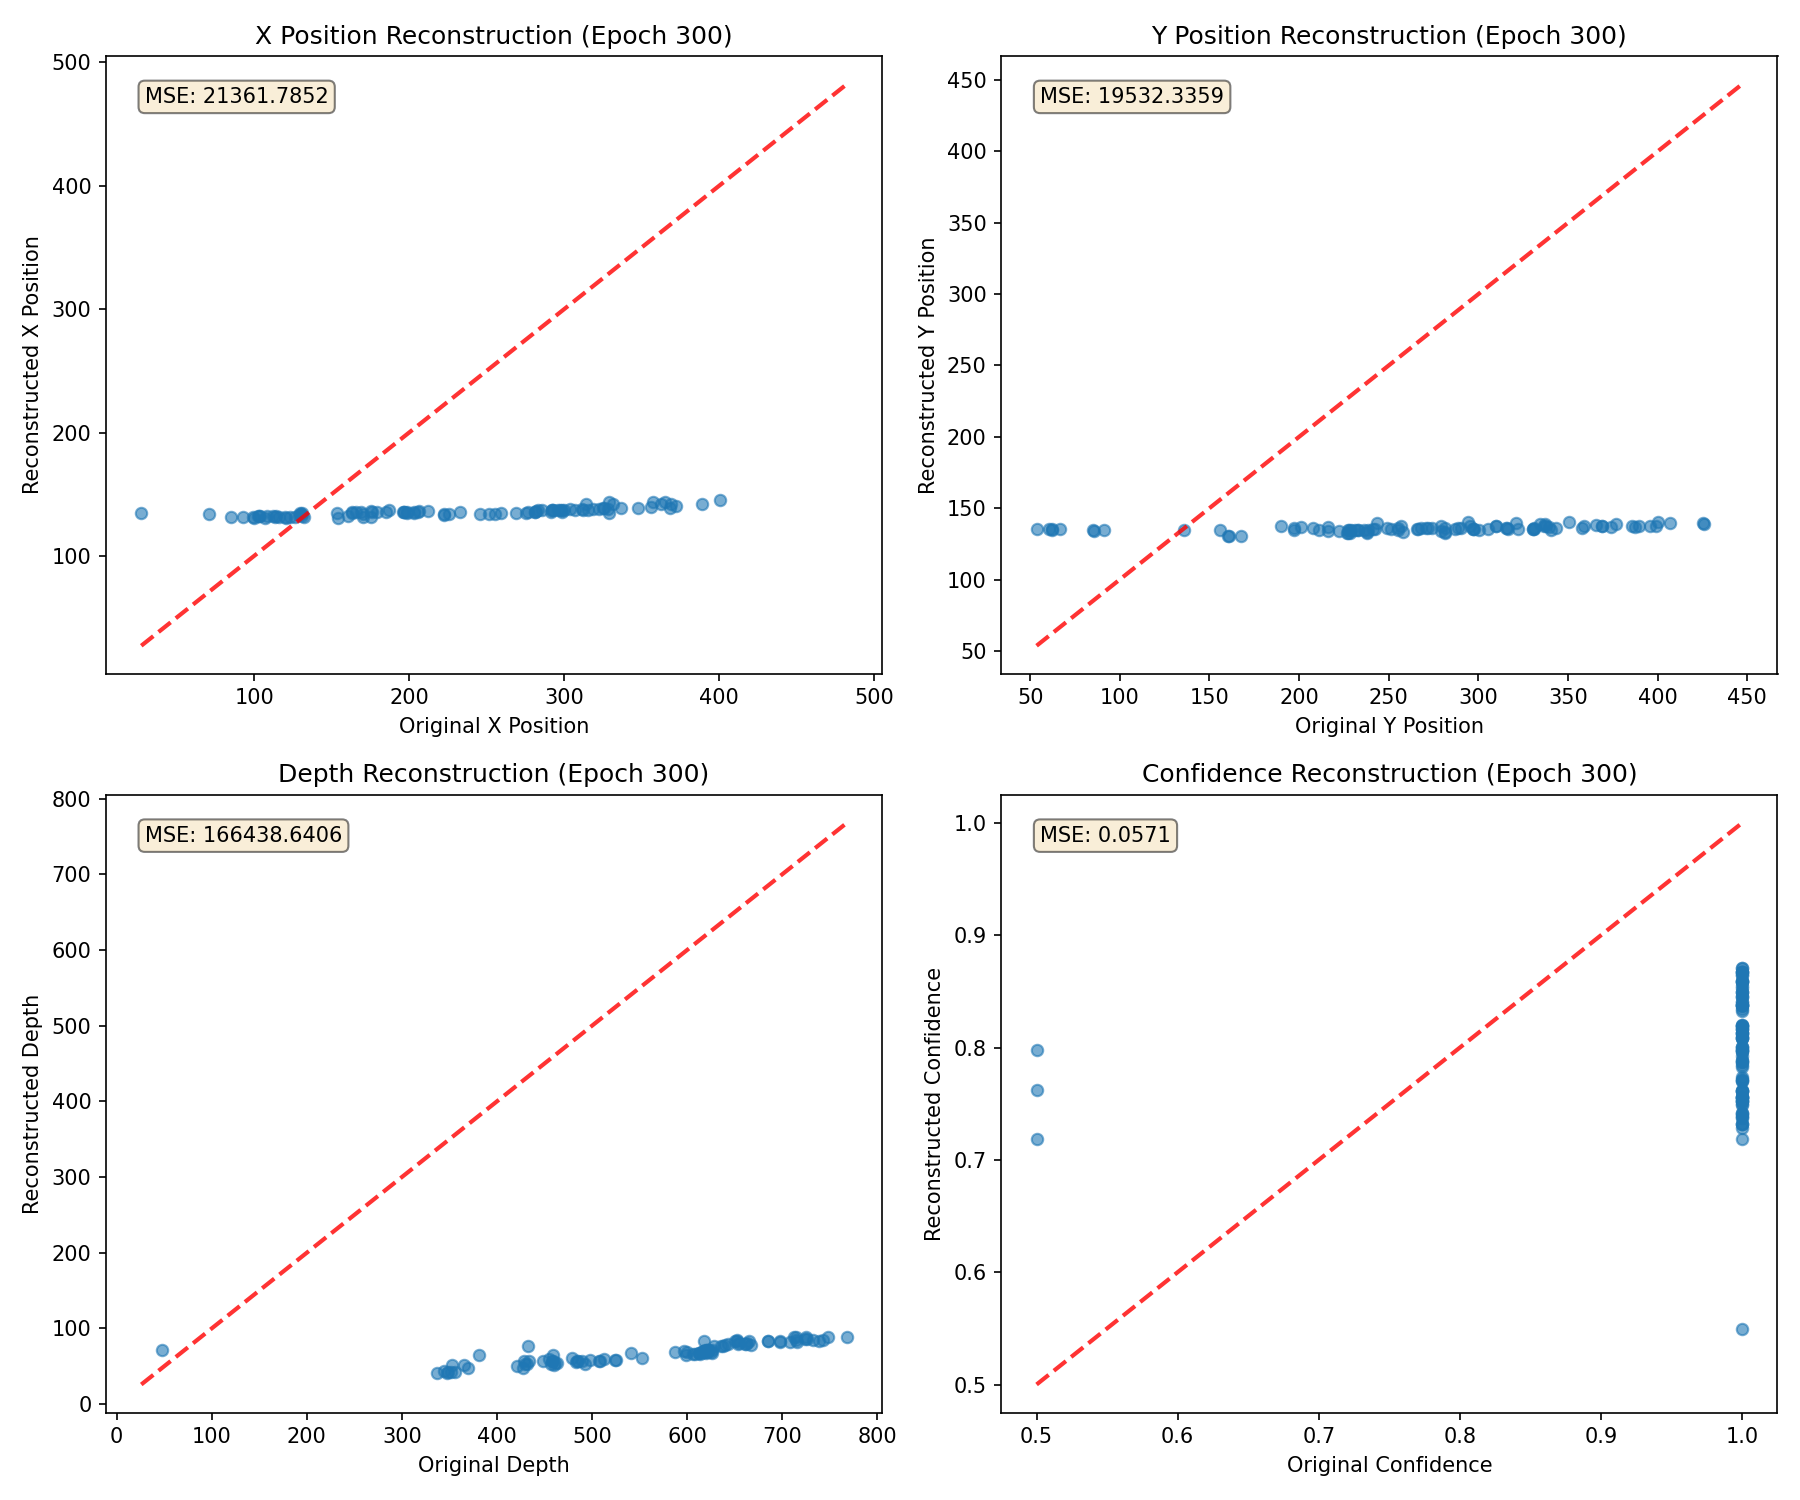
\includegraphics[width=0.4\linewidth]{figures/training_attempt_1/reconstruction_epoch_300.png}
	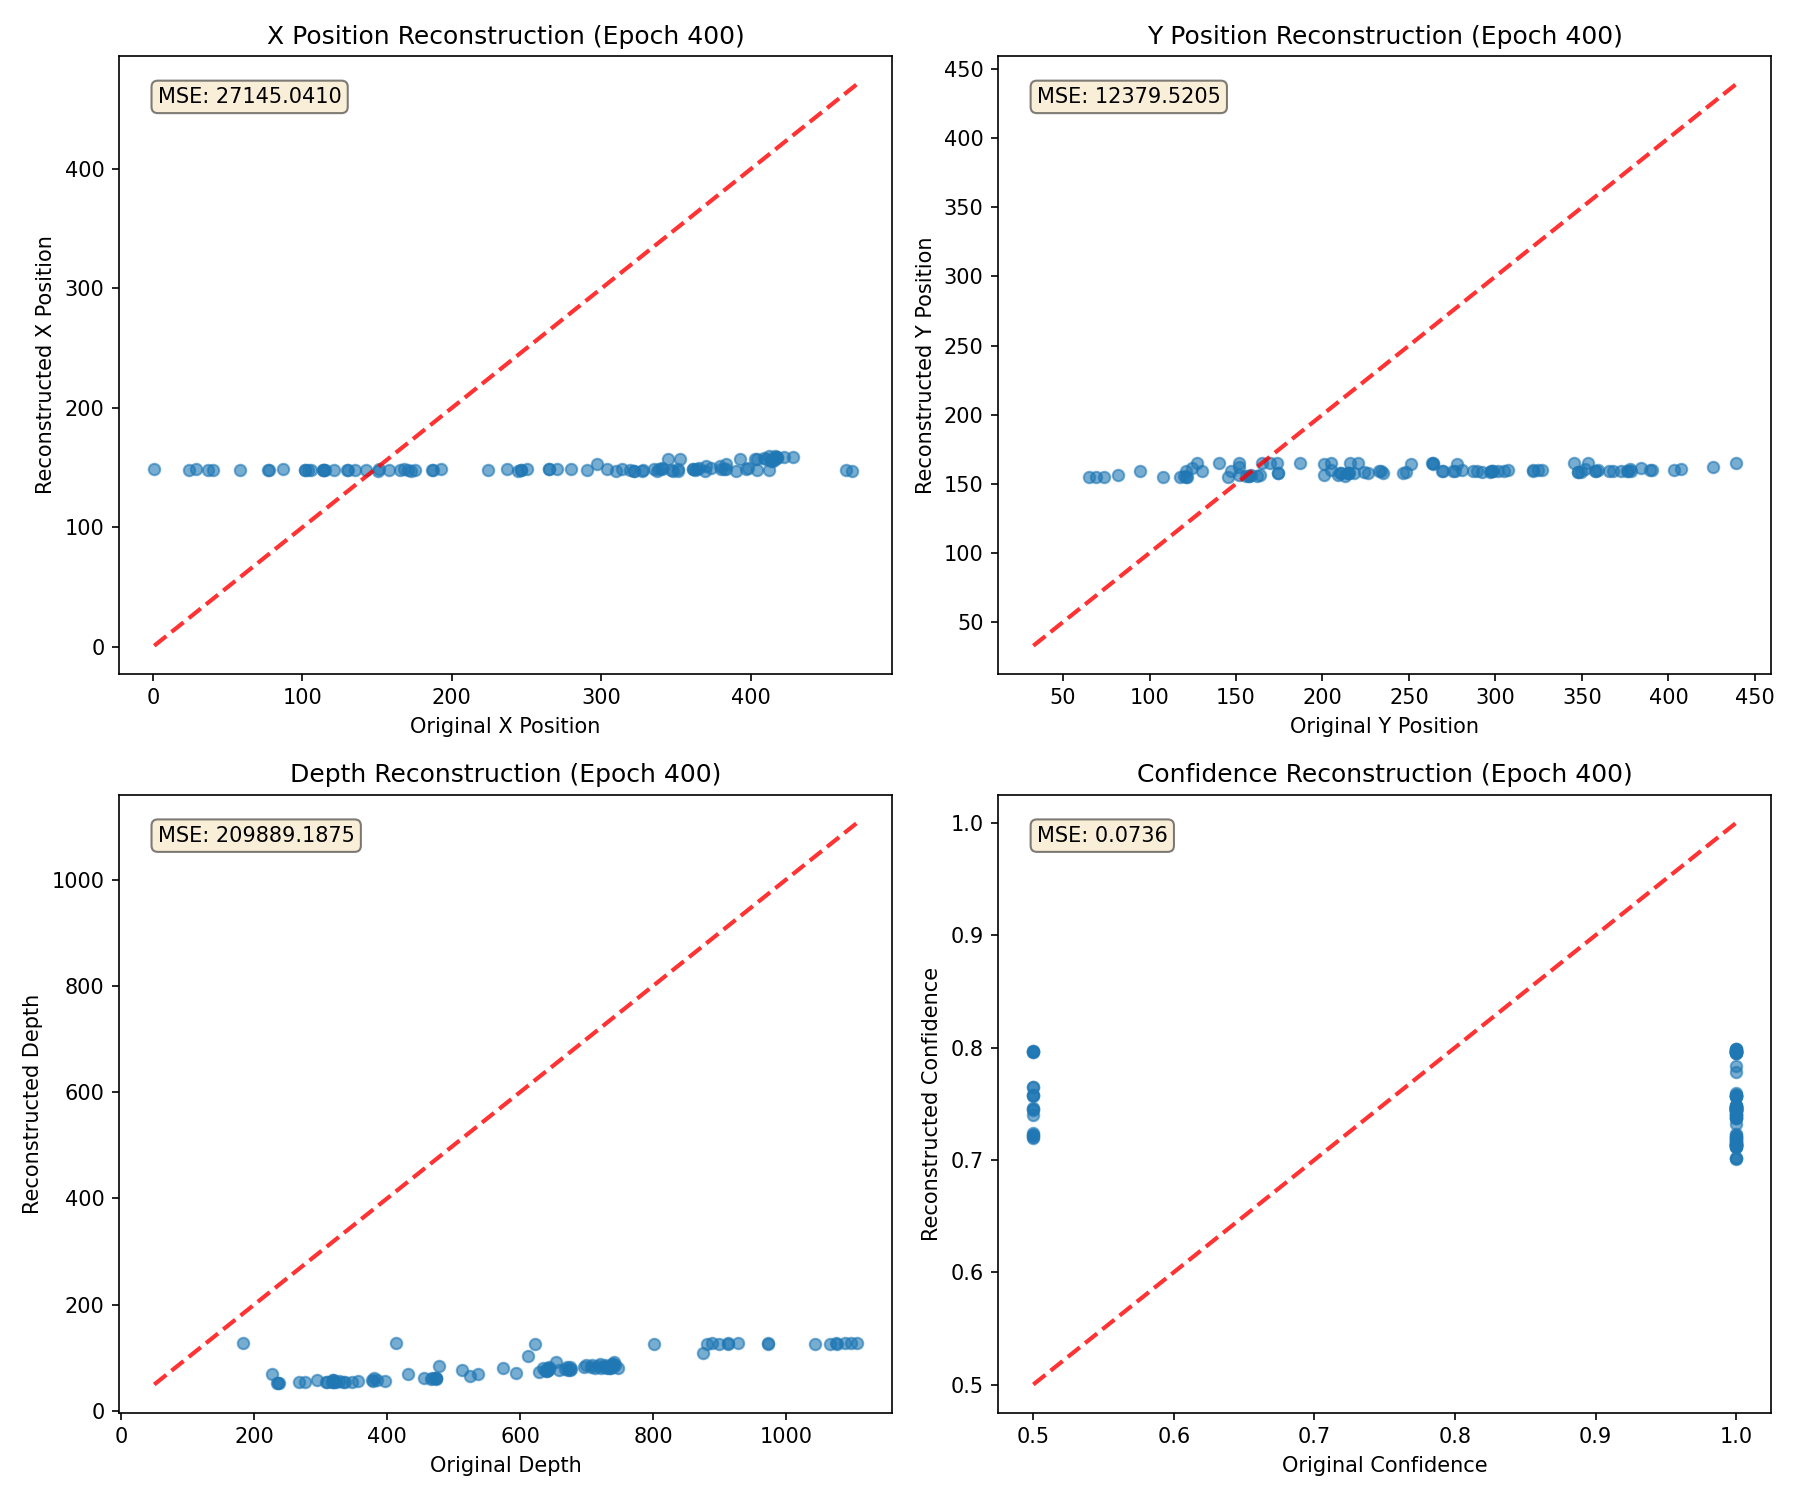
\includegraphics[width=0.4\linewidth]{figures/training_attempt_1/reconstruction_epoch_400.png}
	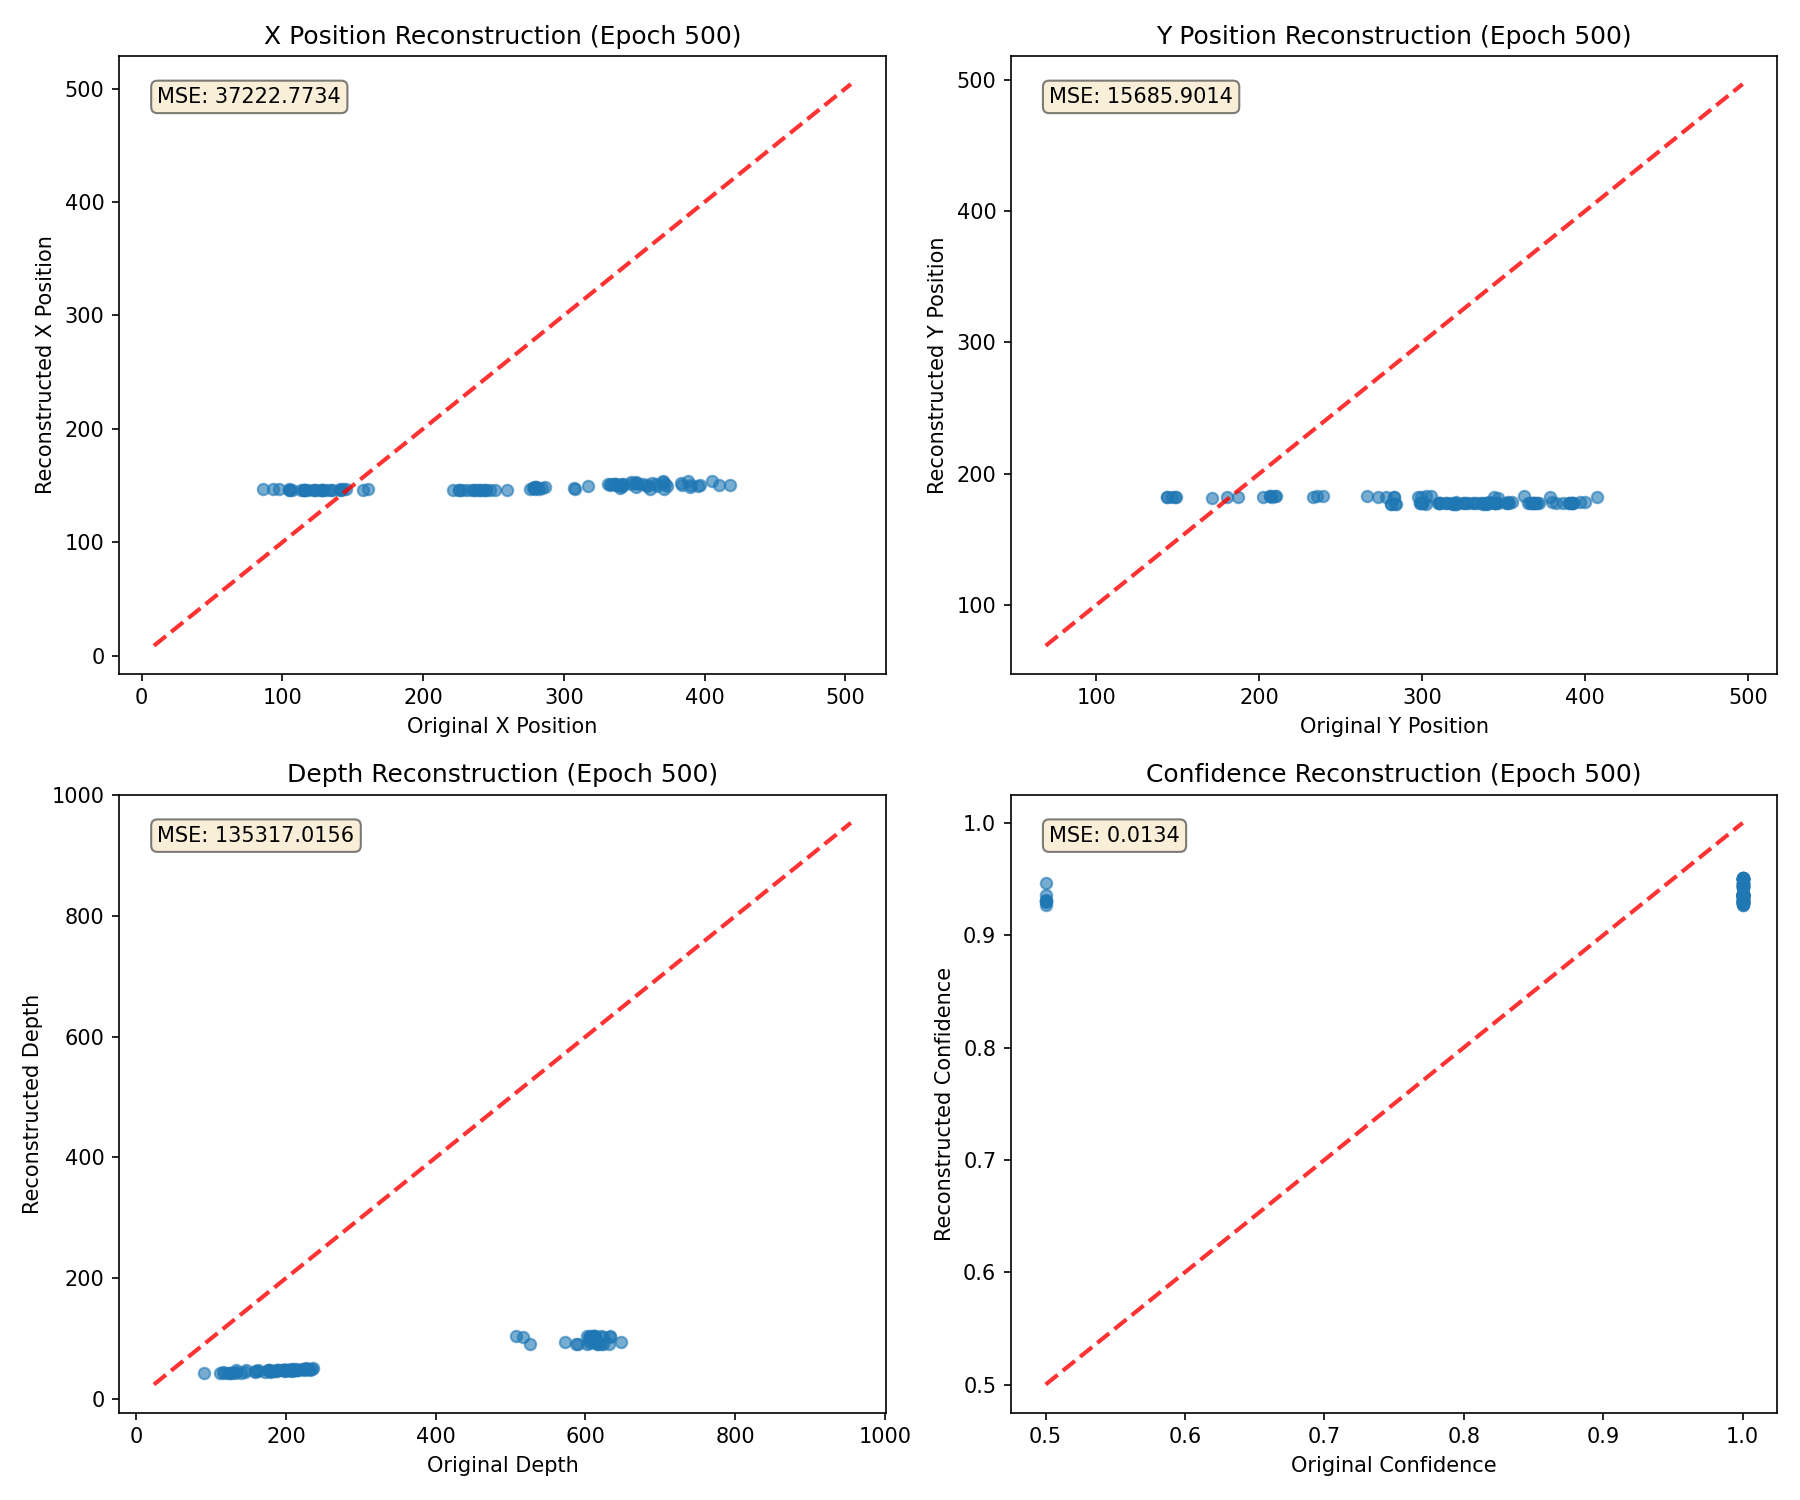
\includegraphics[width=0.4\linewidth]{figures/training_attempt_1/reconstruction_epoch_500.png}
	\caption{Trainign with full set and 500 epochs reconstruction}
	\label{fig:training_attempt_1_reconstruction_epocs}
\end{figure}

Second attempt at training with the full training set and 1500 epochs

\begin{figure}[H]
	\centering
	
\includegraphics[width=0.4\linewidth]{figures/training_attempt_2/embeddings_epoch_100.png}
	
\includegraphics[width=0.4\linewidth]{figures/training_attempt_2/embeddings_epoch_200.png}
	
\includegraphics[width=0.4\linewidth]{figures/training_attempt_2/embeddings_epoch_300.png}
	
\includegraphics[width=0.4\linewidth]{figures/training_attempt_2/embeddings_epoch_400.png}
	
\includegraphics[width=0.4\linewidth]{figures/training_attempt_2/embeddings_epoch_500.png}
	\caption{Training with full set and 1500 epochs embeddings part 1}
	\label{fig:training_attempt_2_embeddings_epocs_part_1}
\end{figure}

\begin{figure}[H]
	\centering
	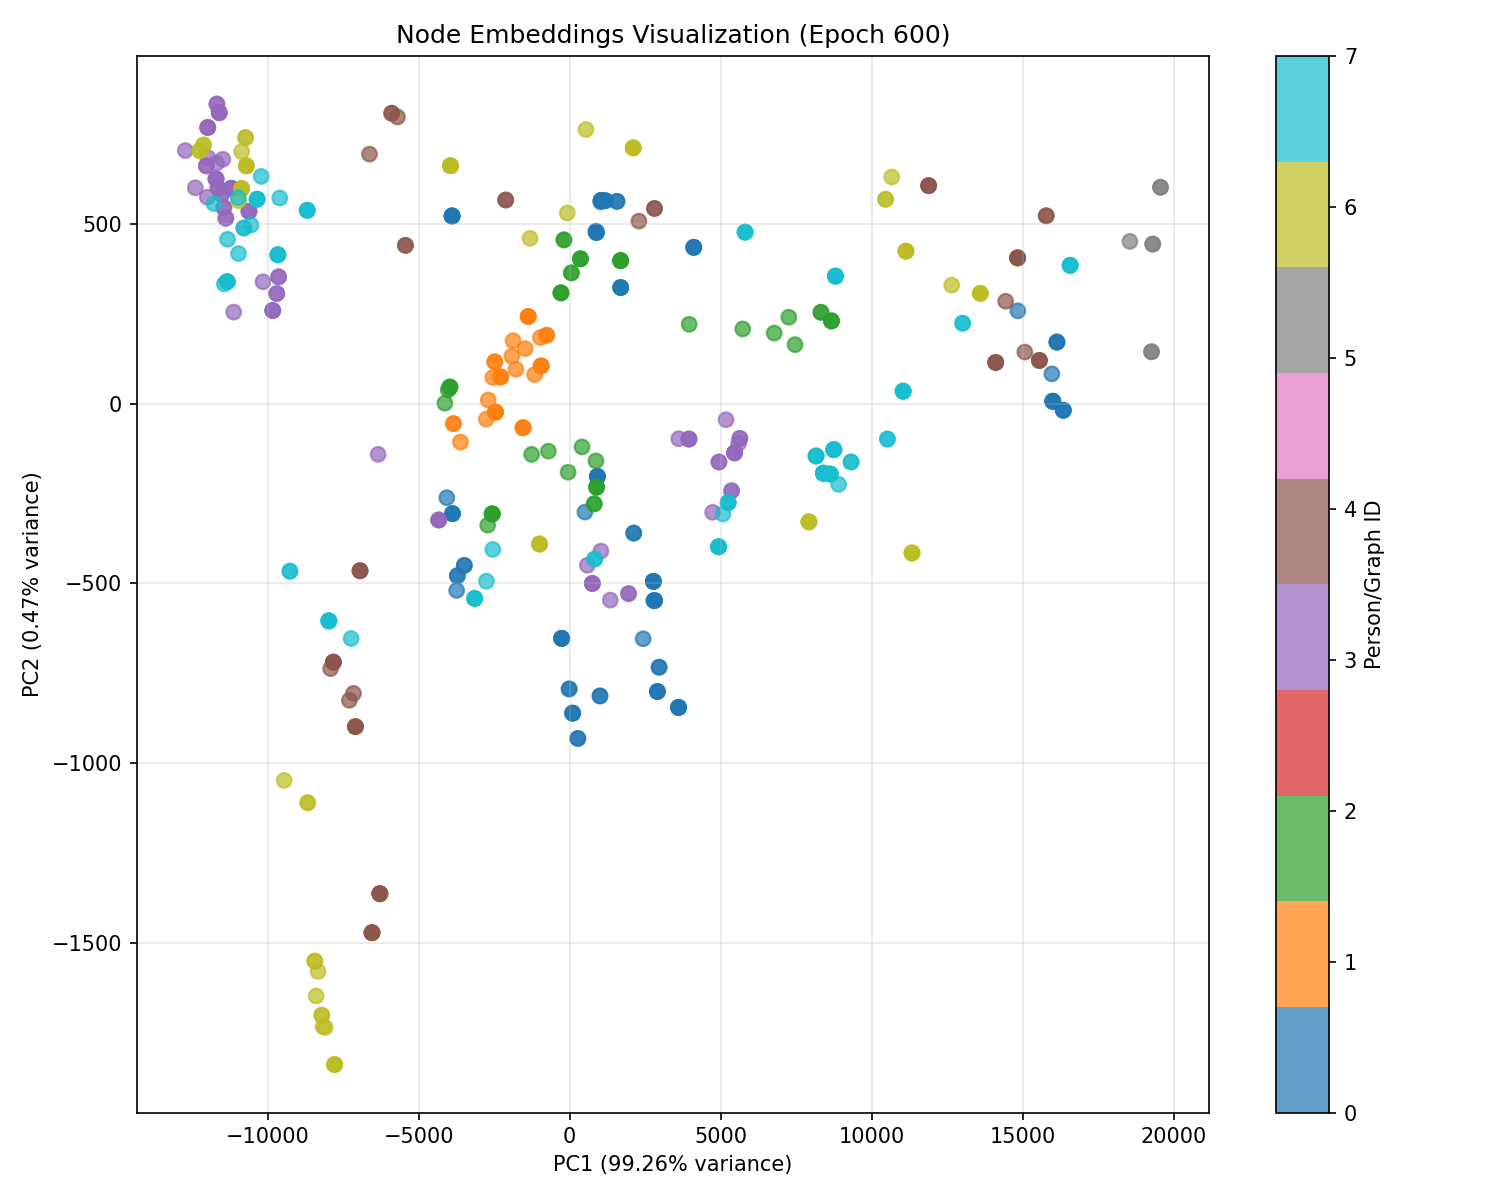
\includegraphics[width=0.4\linewidth]{figures/training_attempt_2/embeddings_epoch_600.png}
	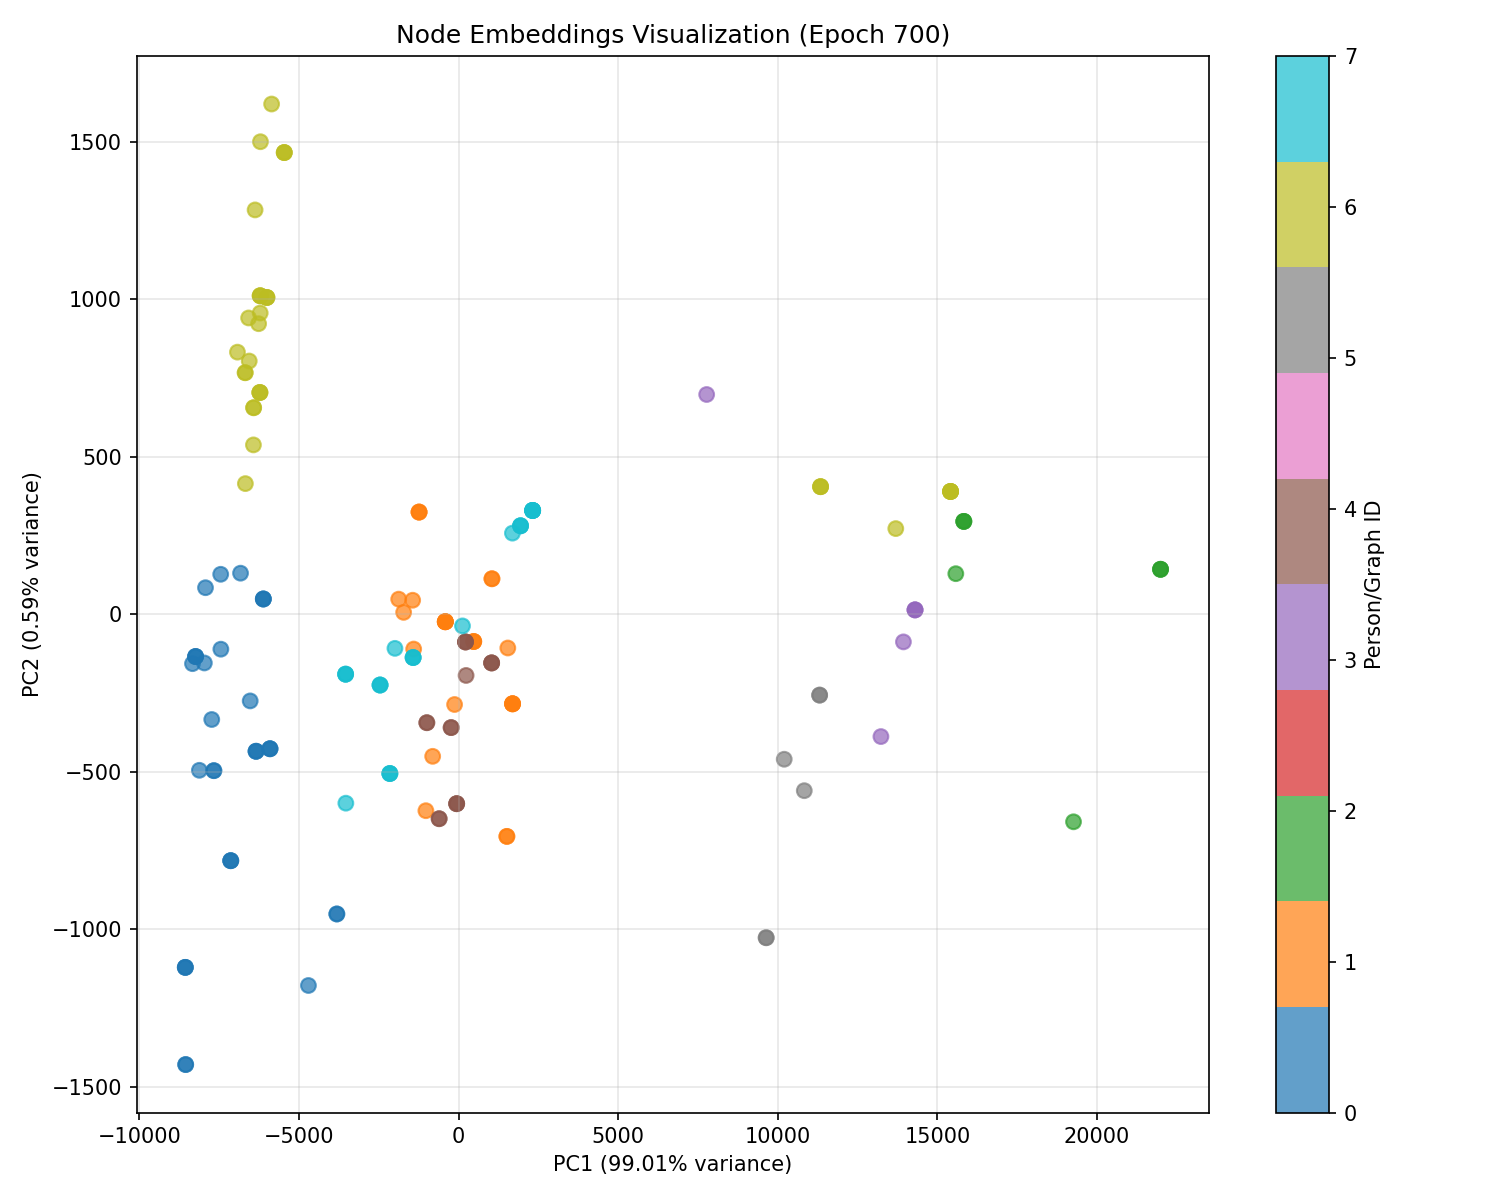
\includegraphics[width=0.4\linewidth]{figures/training_attempt_2/embeddings_epoch_700.png}
	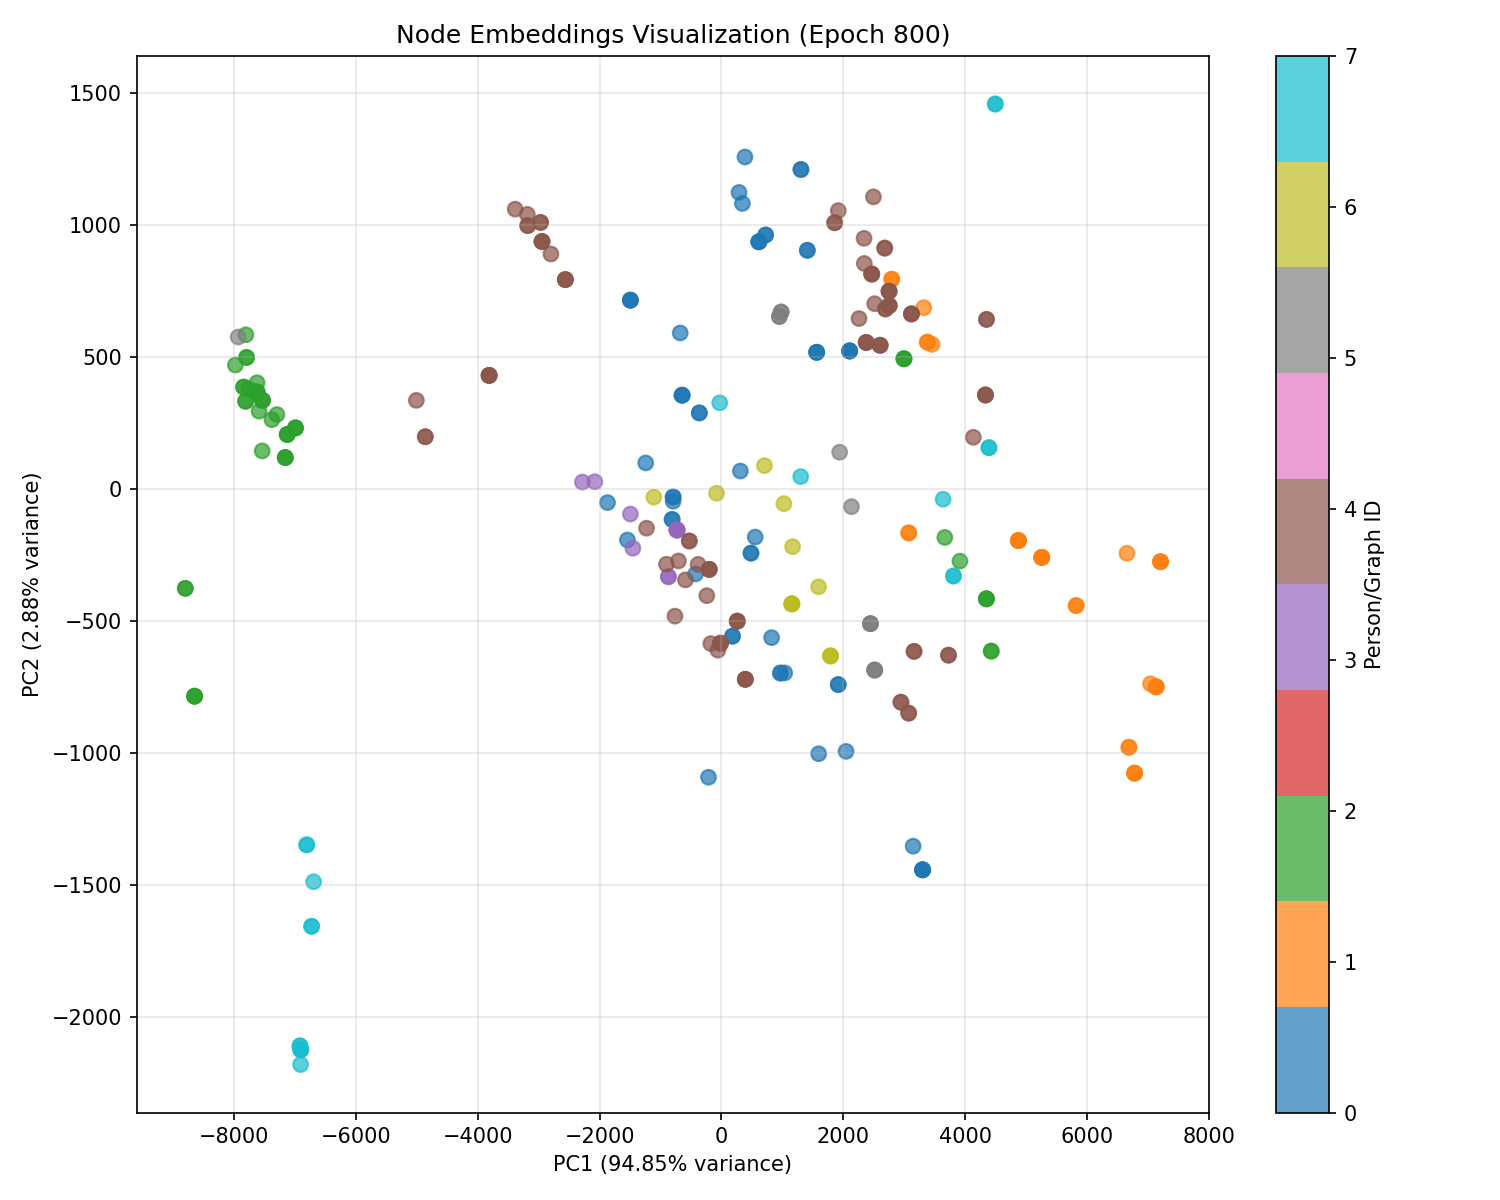
\includegraphics[width=0.4\linewidth]{figures/training_attempt_2/embeddings_epoch_800.png}
	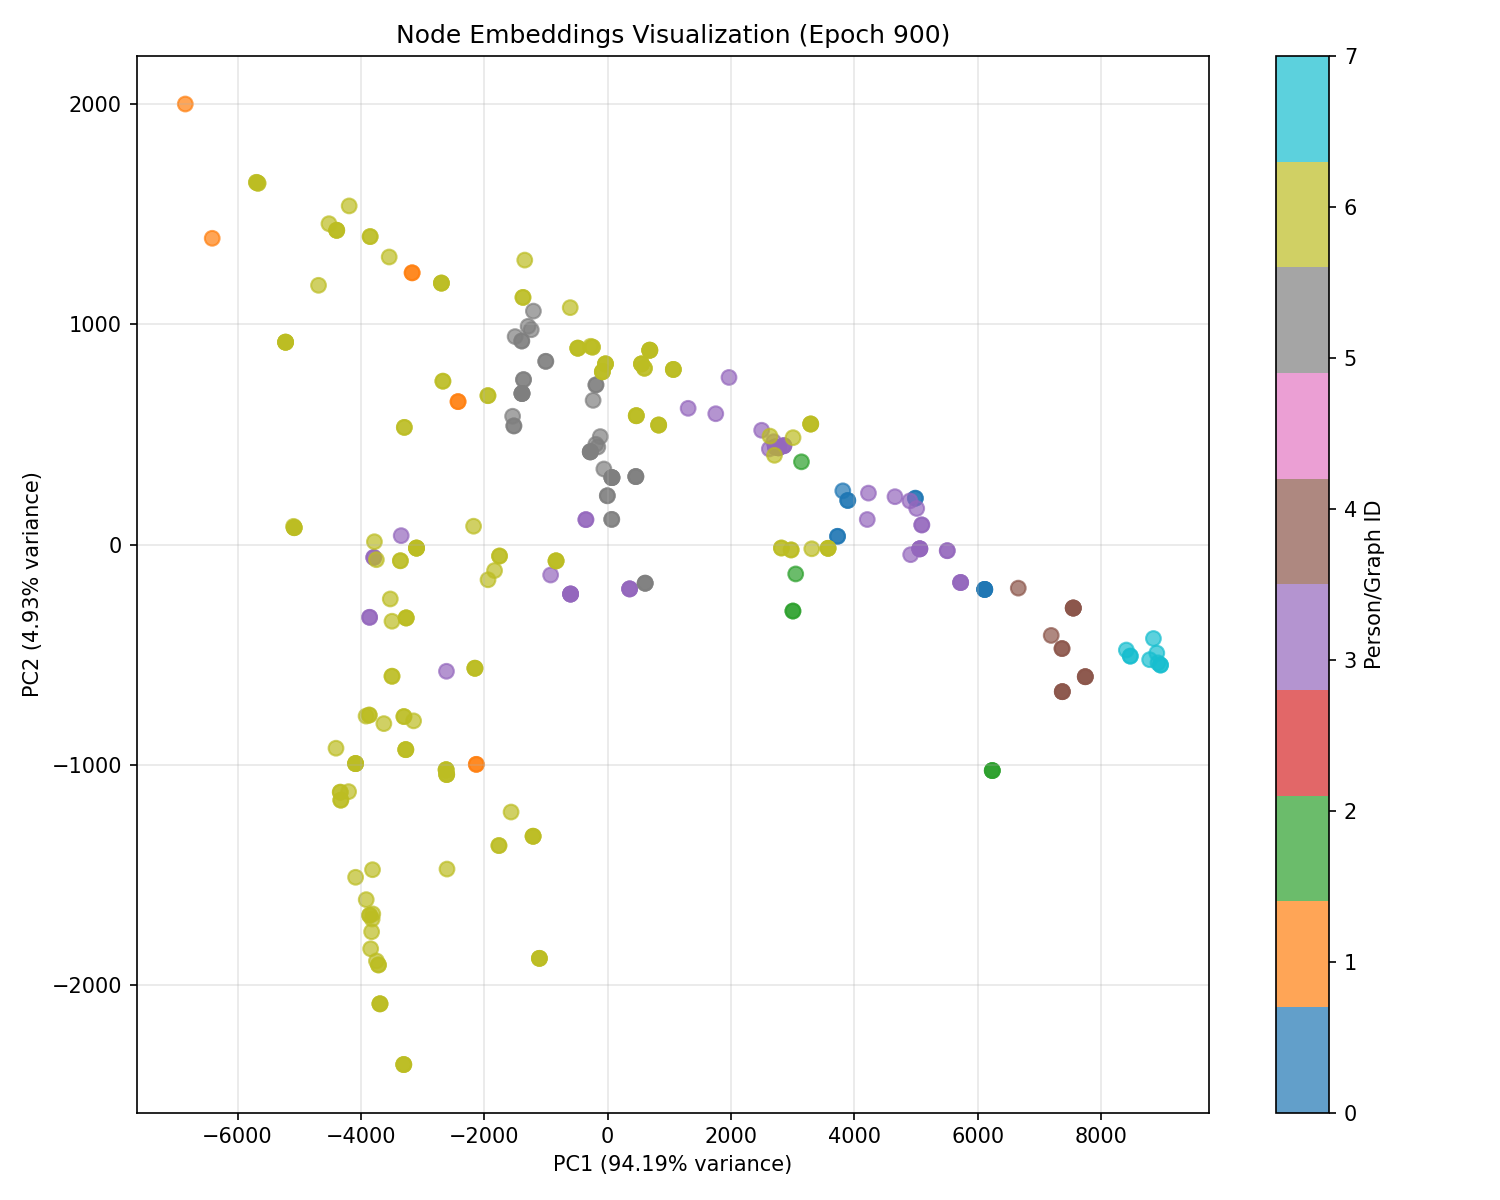
\includegraphics[width=0.4\linewidth]{figures/training_attempt_2/embeddings_epoch_900.png}
	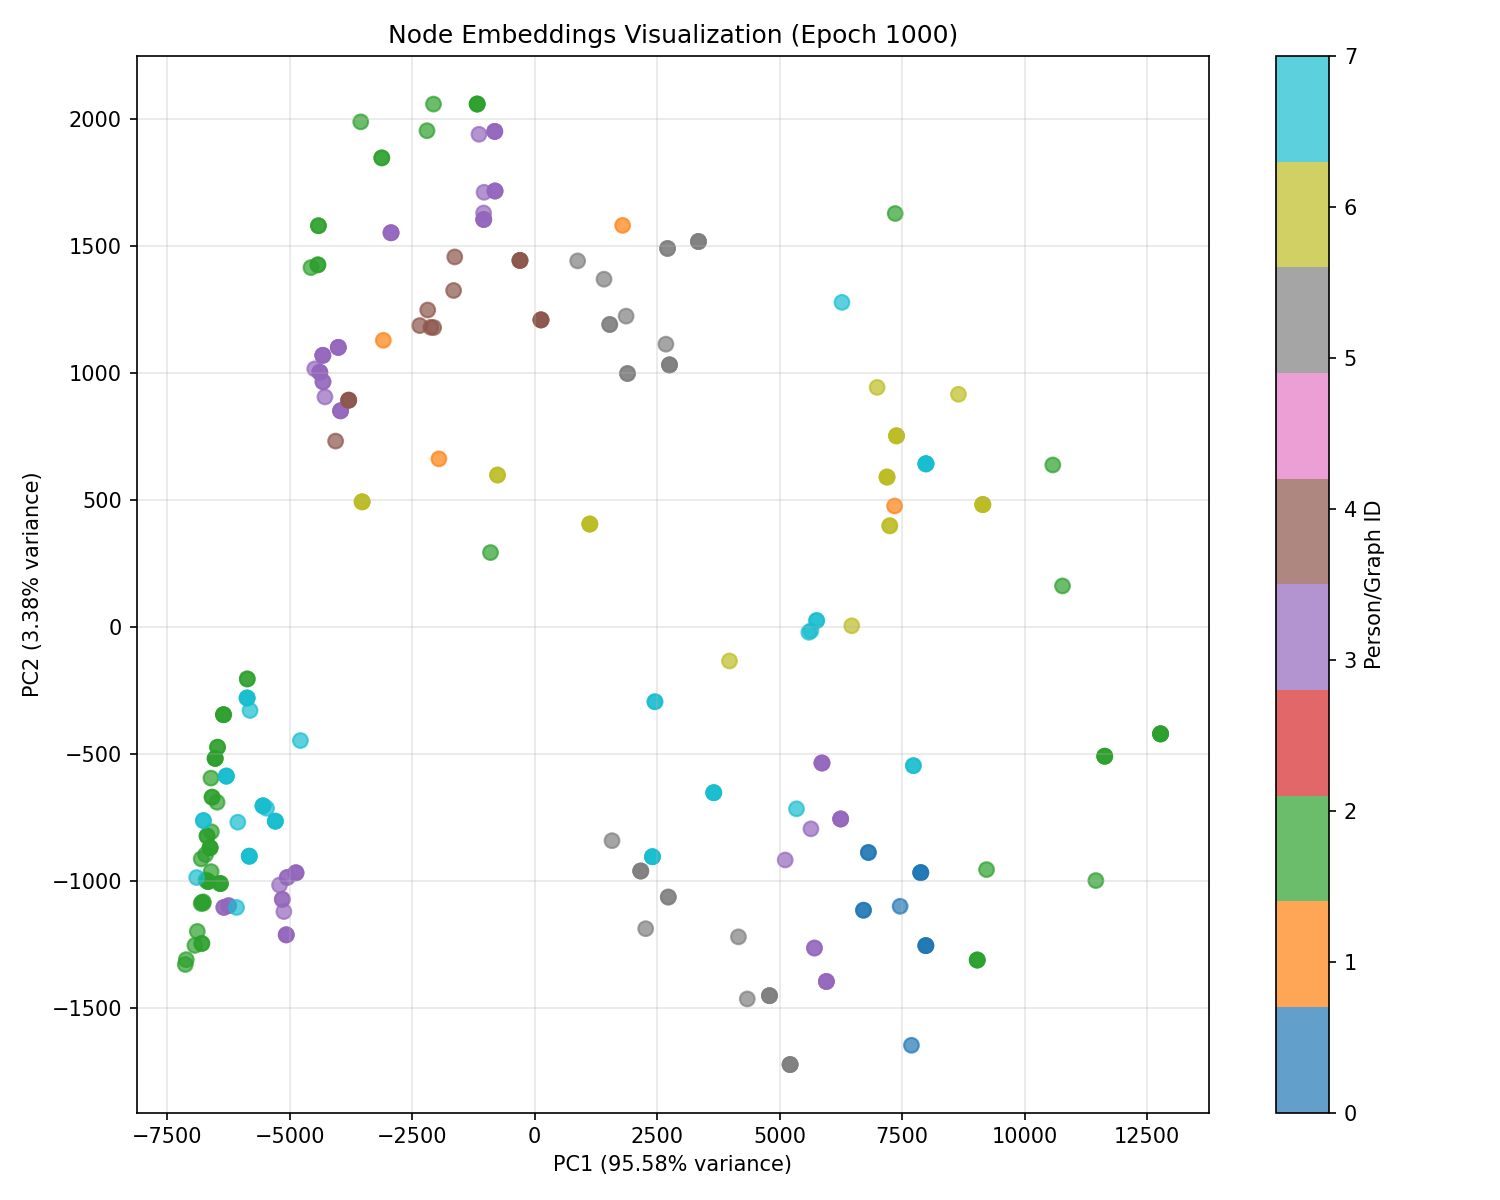
\includegraphics[width=0.4\linewidth]{figures/training_attempt_2/embeddings_epoch_1000.png}
	\caption{Training with full set and 1500 epochs embeddings part 2}
	\label{fig:training_attempt_2_embeddings_epocs_part_2}
\end{figure}

\begin{figure}[H]
	\centering
	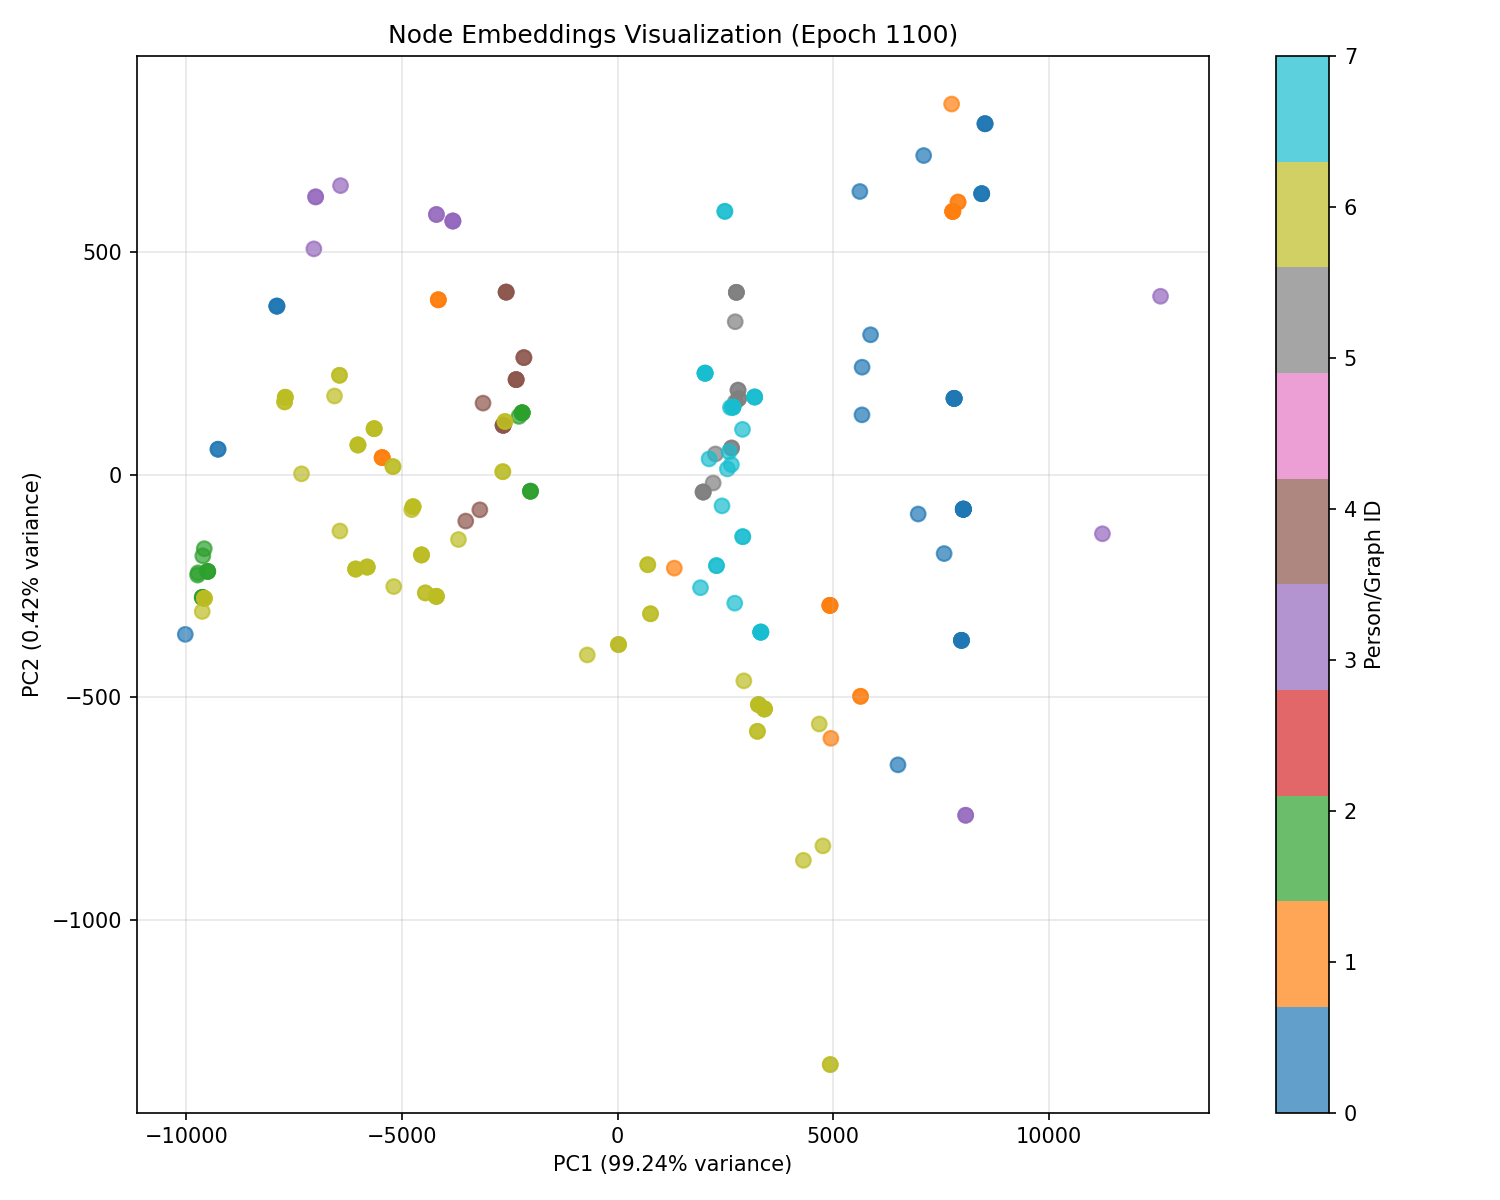
\includegraphics[width=0.4\linewidth]{figures/training_attempt_2/embeddings_epoch_1100.png}
	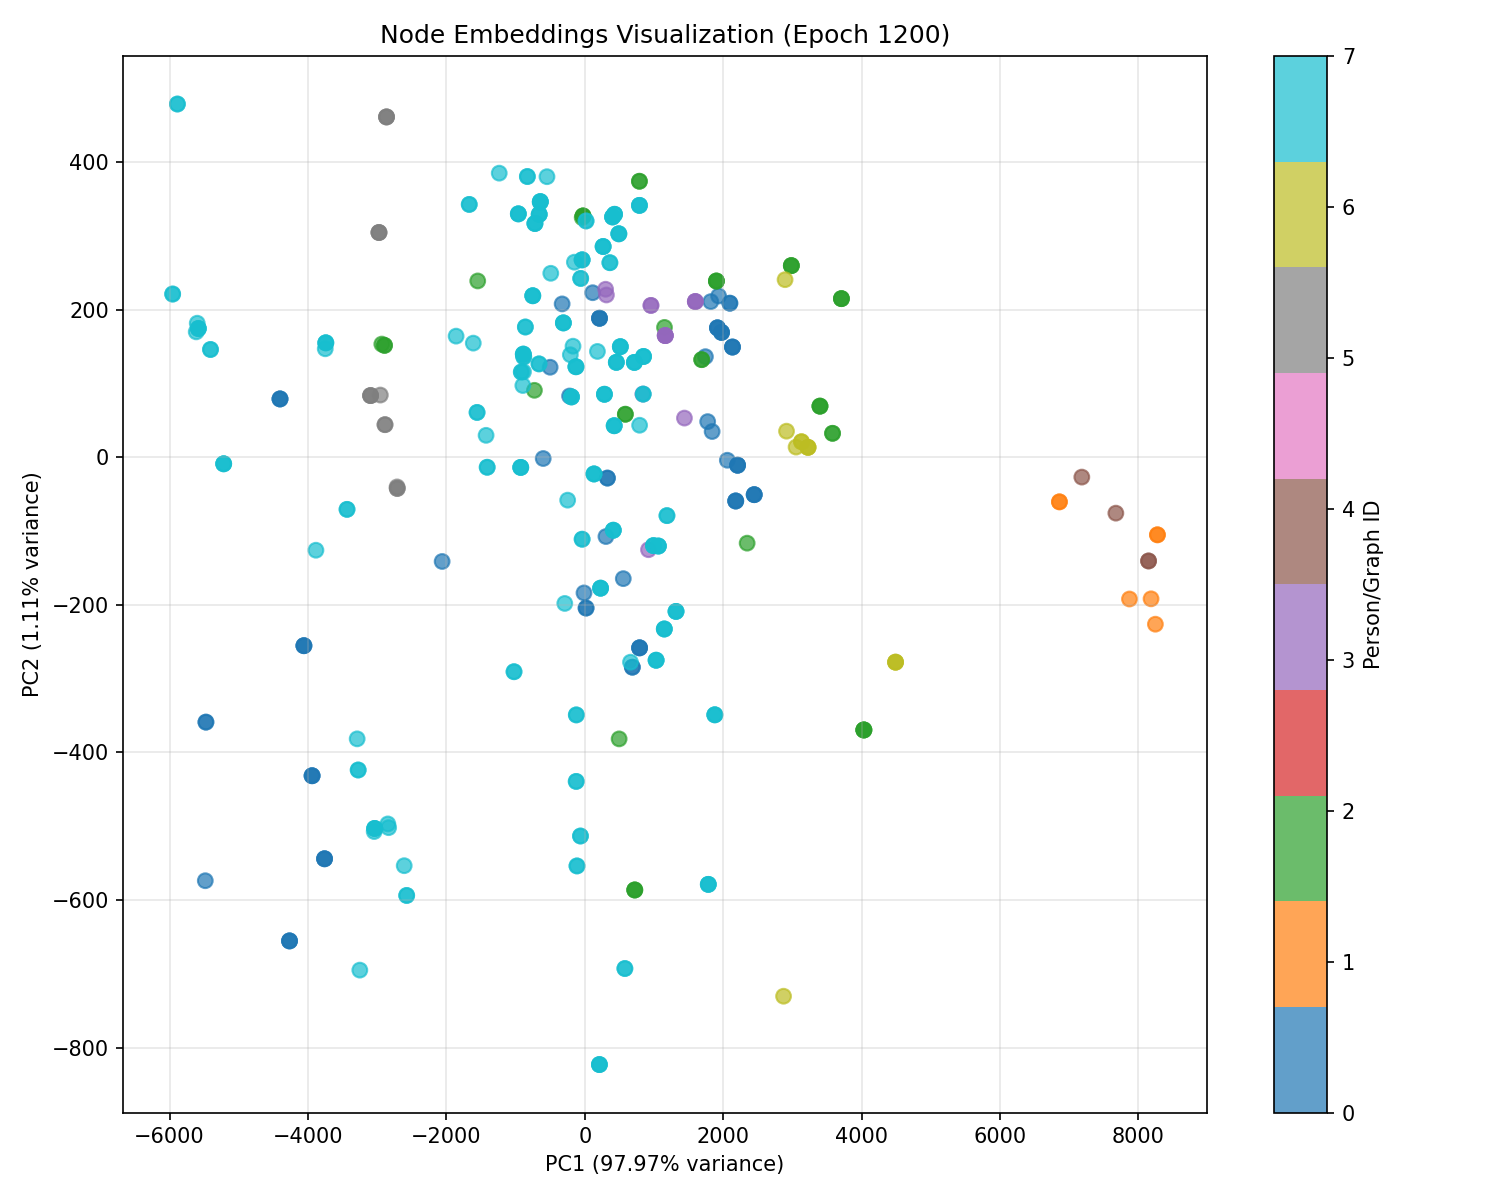
\includegraphics[width=0.4\linewidth]{figures/training_attempt_2/embeddings_epoch_1200.png}
	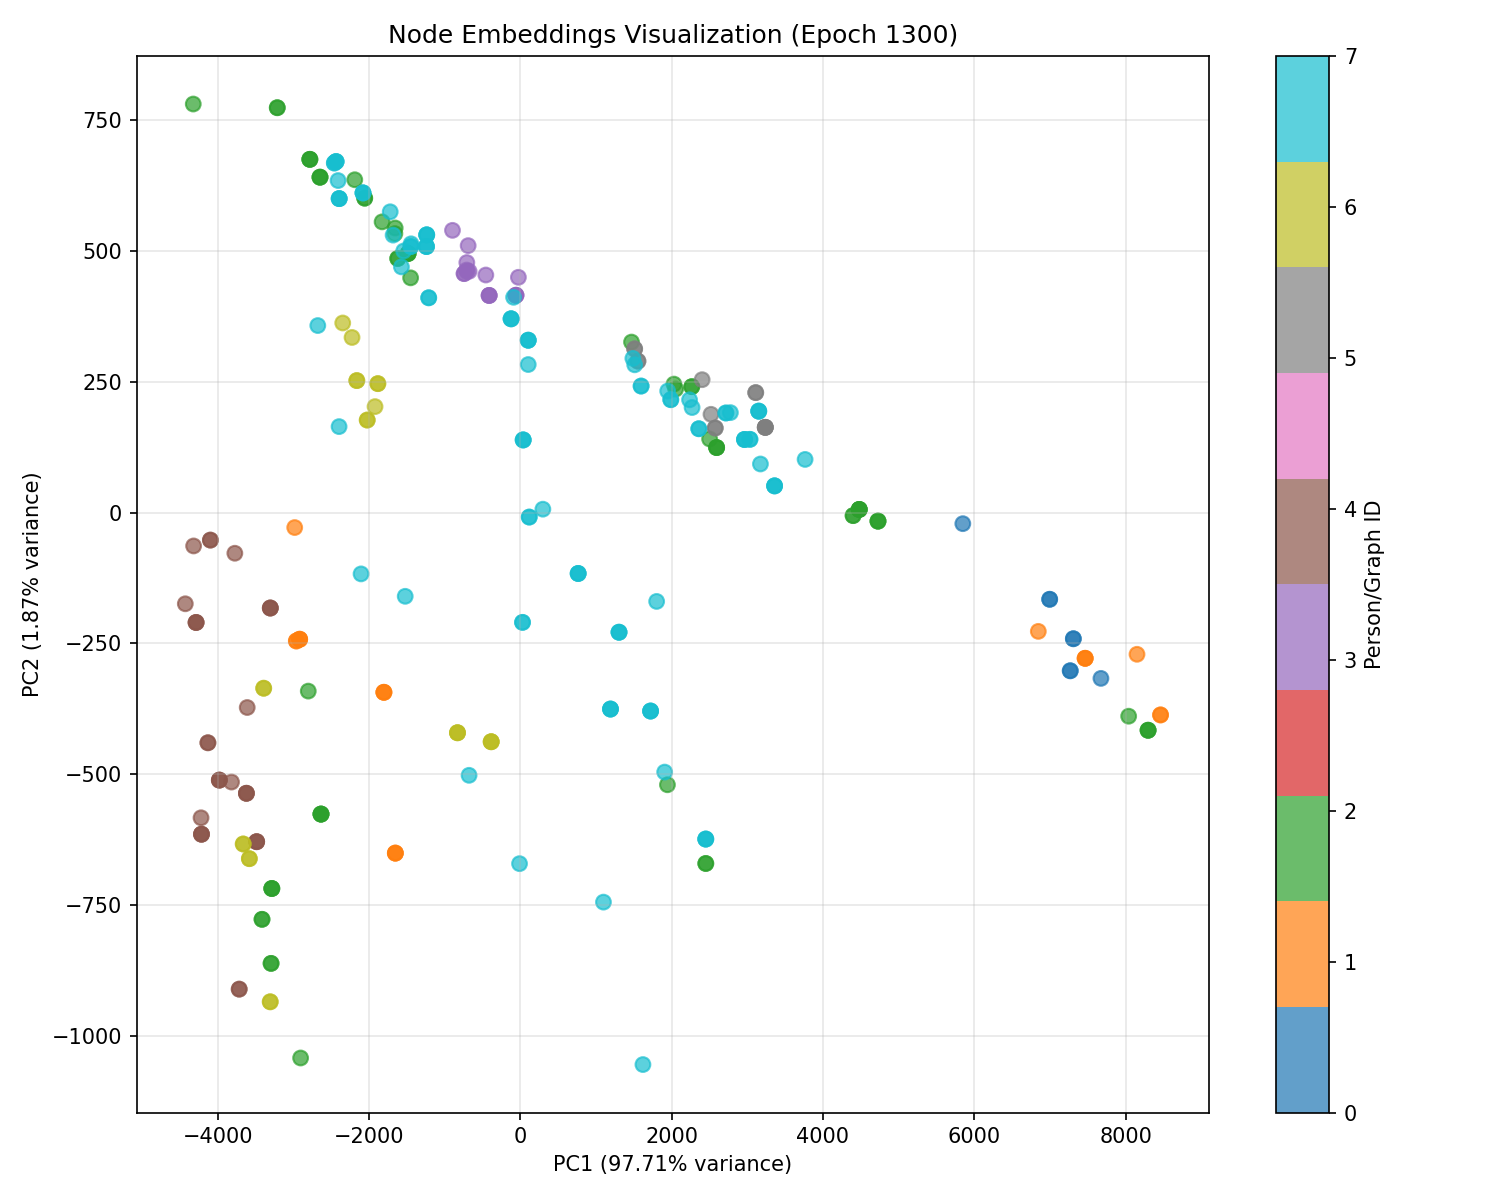
\includegraphics[width=0.4\linewidth]{figures/training_attempt_2/embeddings_epoch_1300.png}
	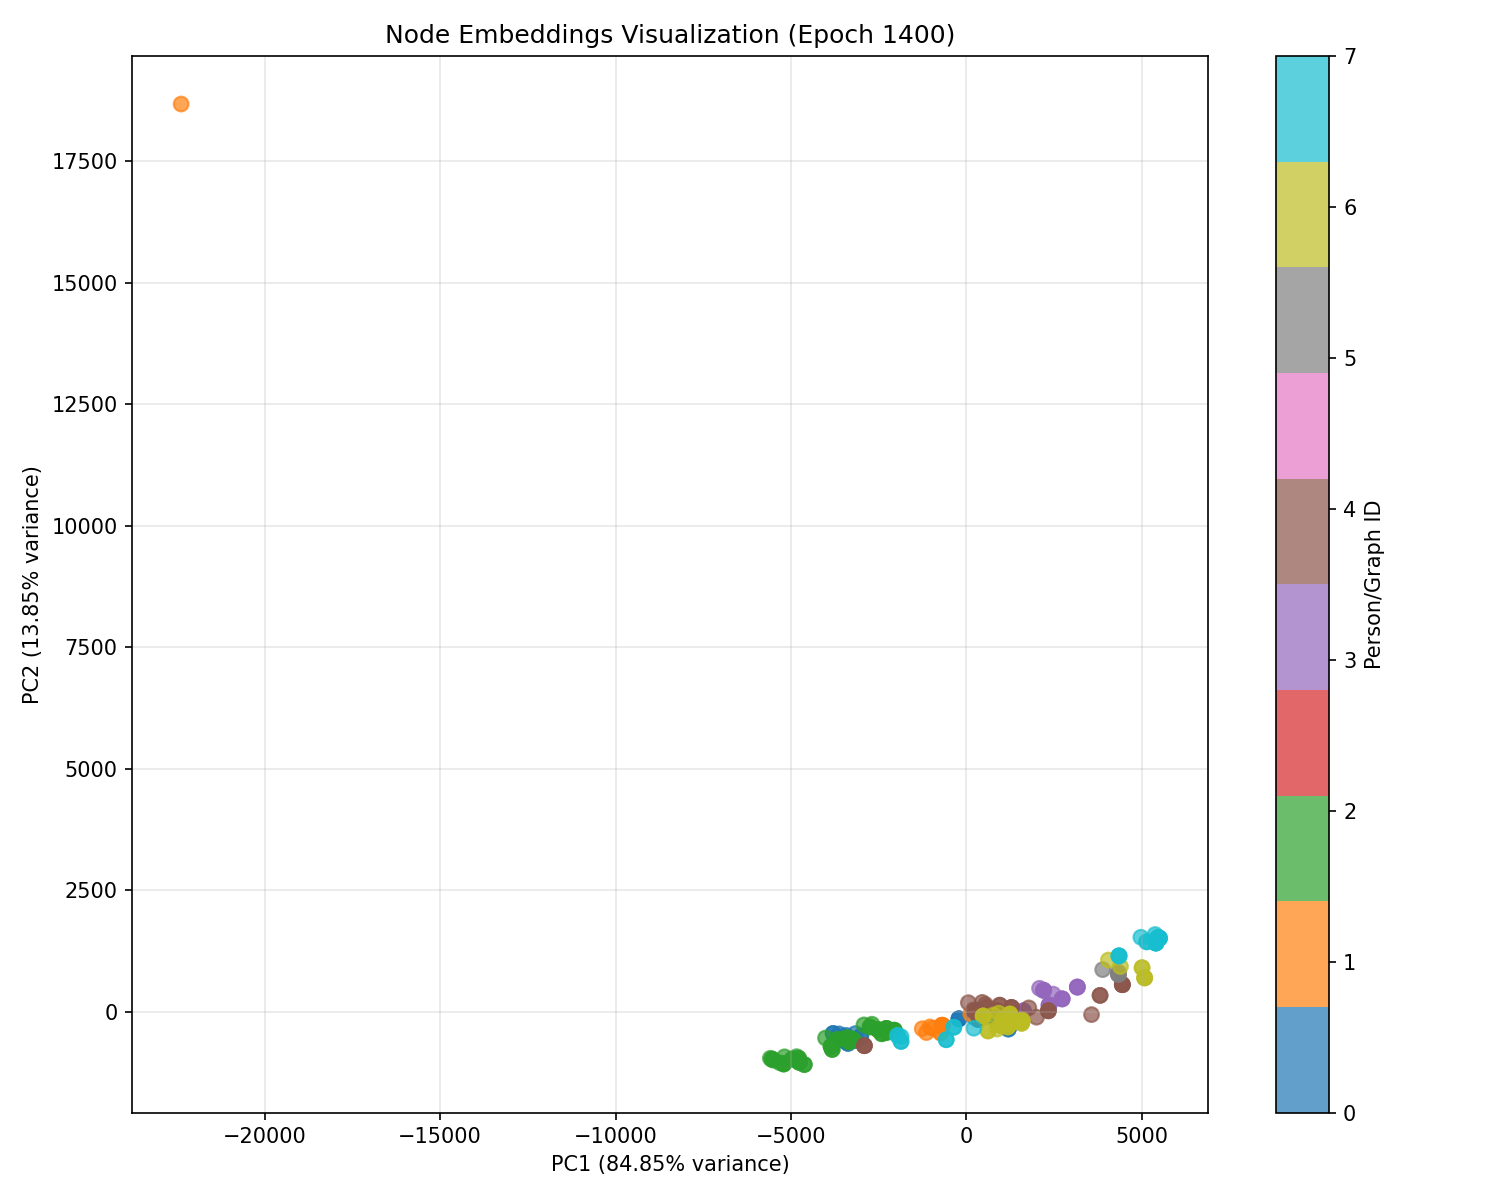
\includegraphics[width=0.4\linewidth]{figures/training_attempt_2/embeddings_epoch_1400.png}
	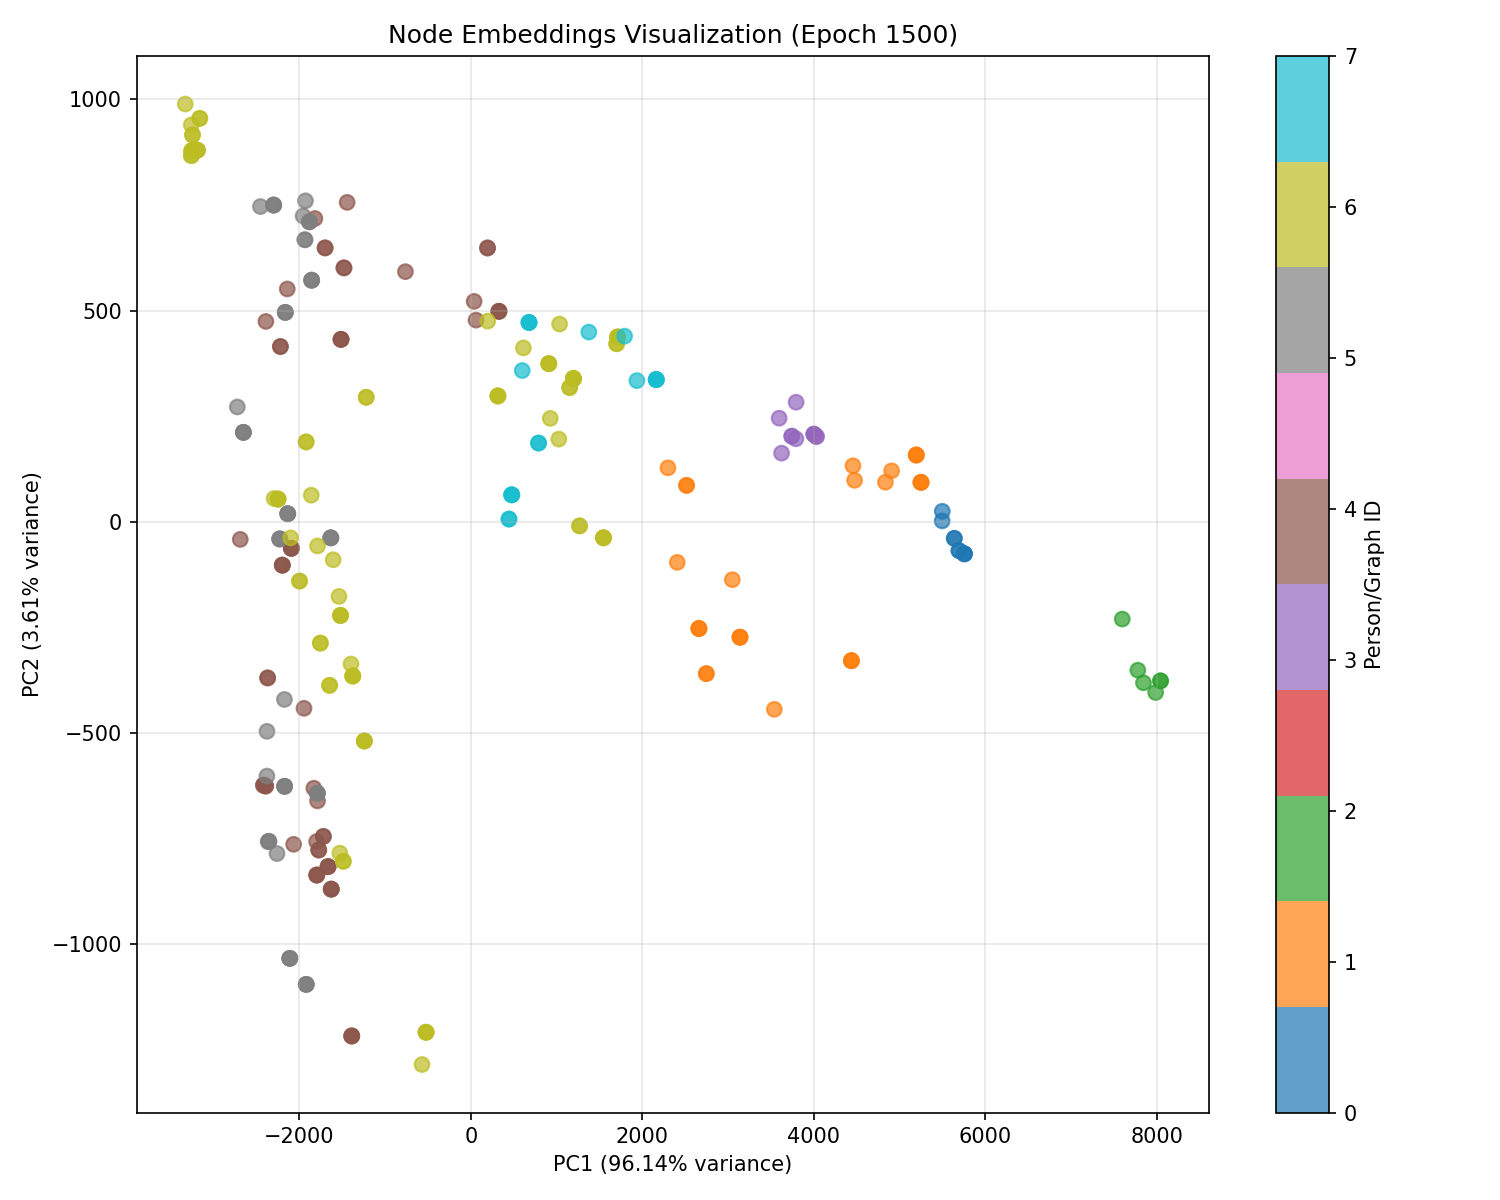
\includegraphics[width=0.4\linewidth]{figures/training_attempt_2/embeddings_epoch_1500.png}
	\caption{Training with full set and 1500 epochs embeddings part 3}
	\label{fig:training_attempt_2_embeddings_epocs_part_3}
\end{figure}

\begin{figure}[H]
	\centering
	
\includegraphics[width=0.4\linewidth]{figures/training_attempt_2/reconstruction_epoch_100.png}
	
\includegraphics[width=0.4\linewidth]{figures/training_attempt_2/reconstruction_epoch_200.png}
	
\includegraphics[width=0.4\linewidth]{figures/training_attempt_2/reconstruction_epoch_300.png}
	
\includegraphics[width=0.4\linewidth]{figures/training_attempt_2/reconstruction_epoch_400.png}
	
\includegraphics[width=0.4\linewidth]{figures/training_attempt_2/reconstruction_epoch_500.png}
	\caption{Training with full set and 1500 epochs reconstruction part 1}
	\label{fig:training_attempt_2_reconstruction_epocs_part_1}
\end{figure}


\begin{figure}[H]
	\centering
	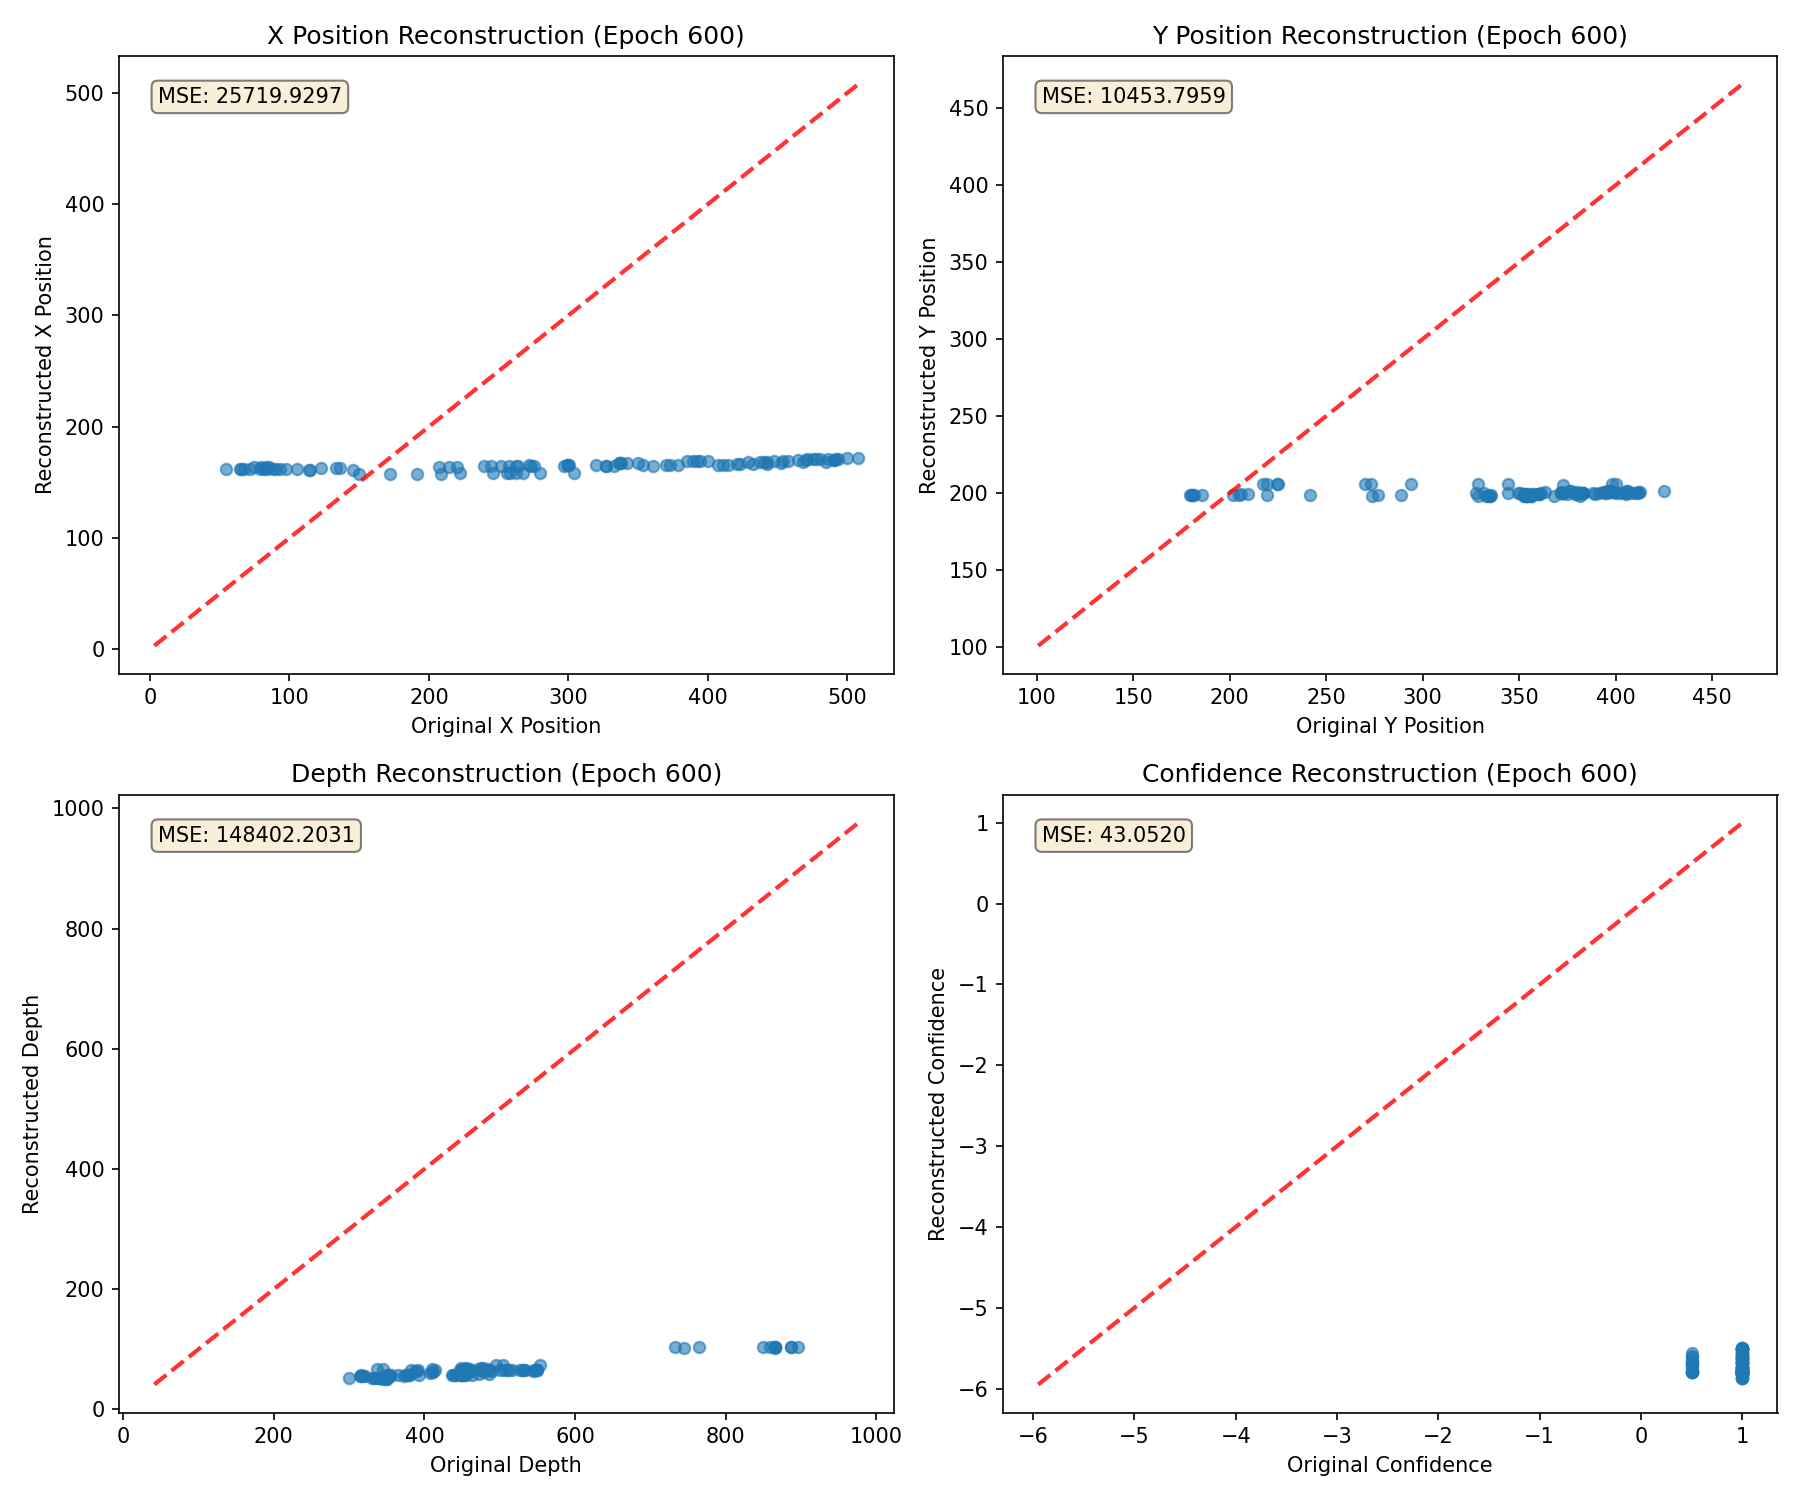
\includegraphics[width=0.4\linewidth]{figures/training_attempt_2/reconstruction_epoch_600.png}
	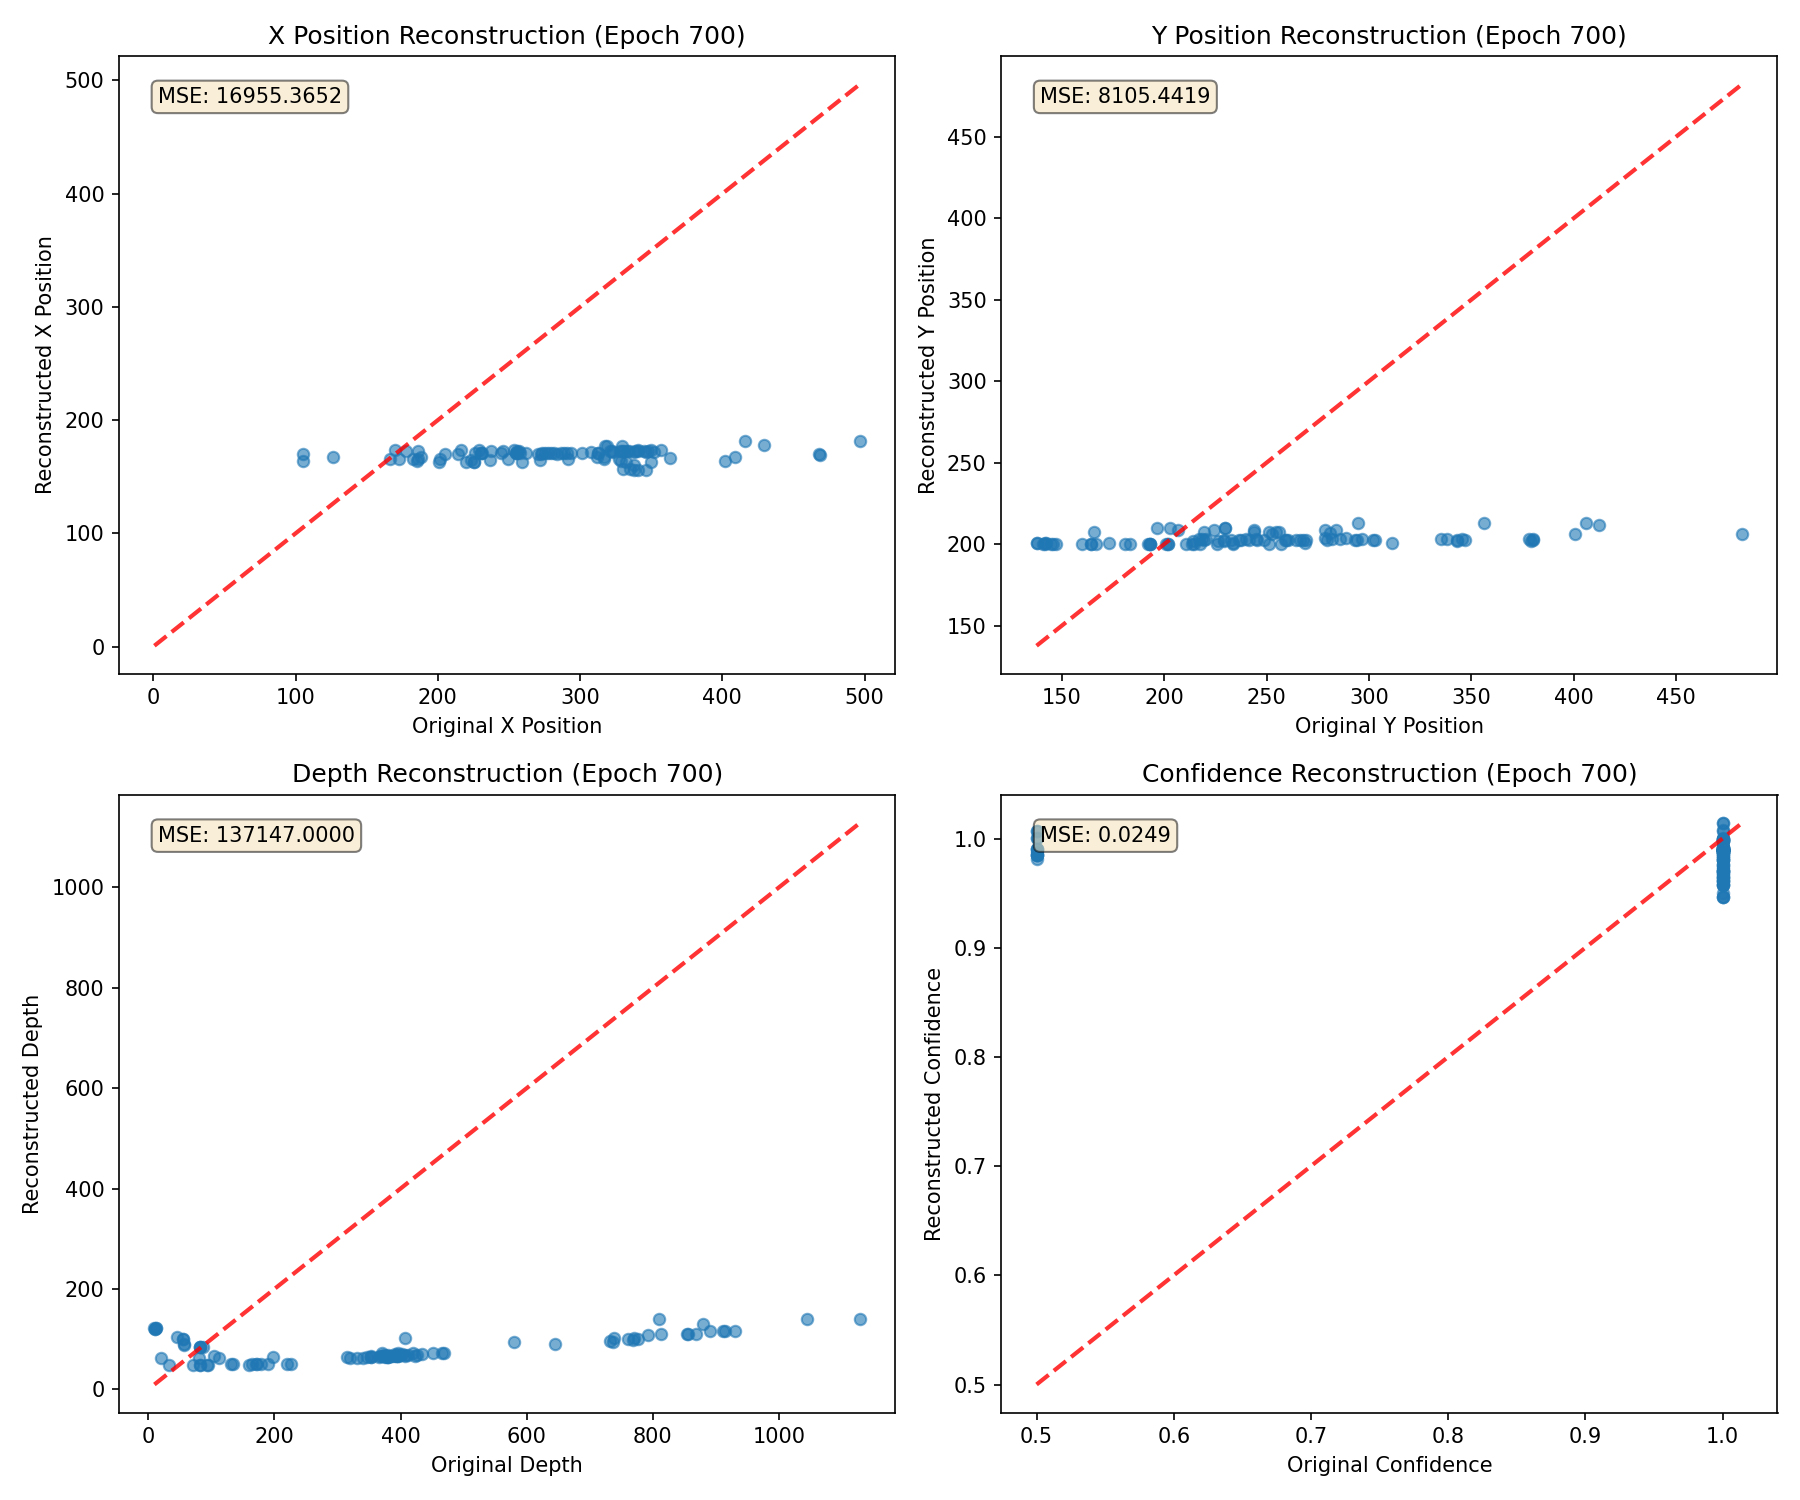
\includegraphics[width=0.4\linewidth]{figures/training_attempt_2/reconstruction_epoch_700.png}
	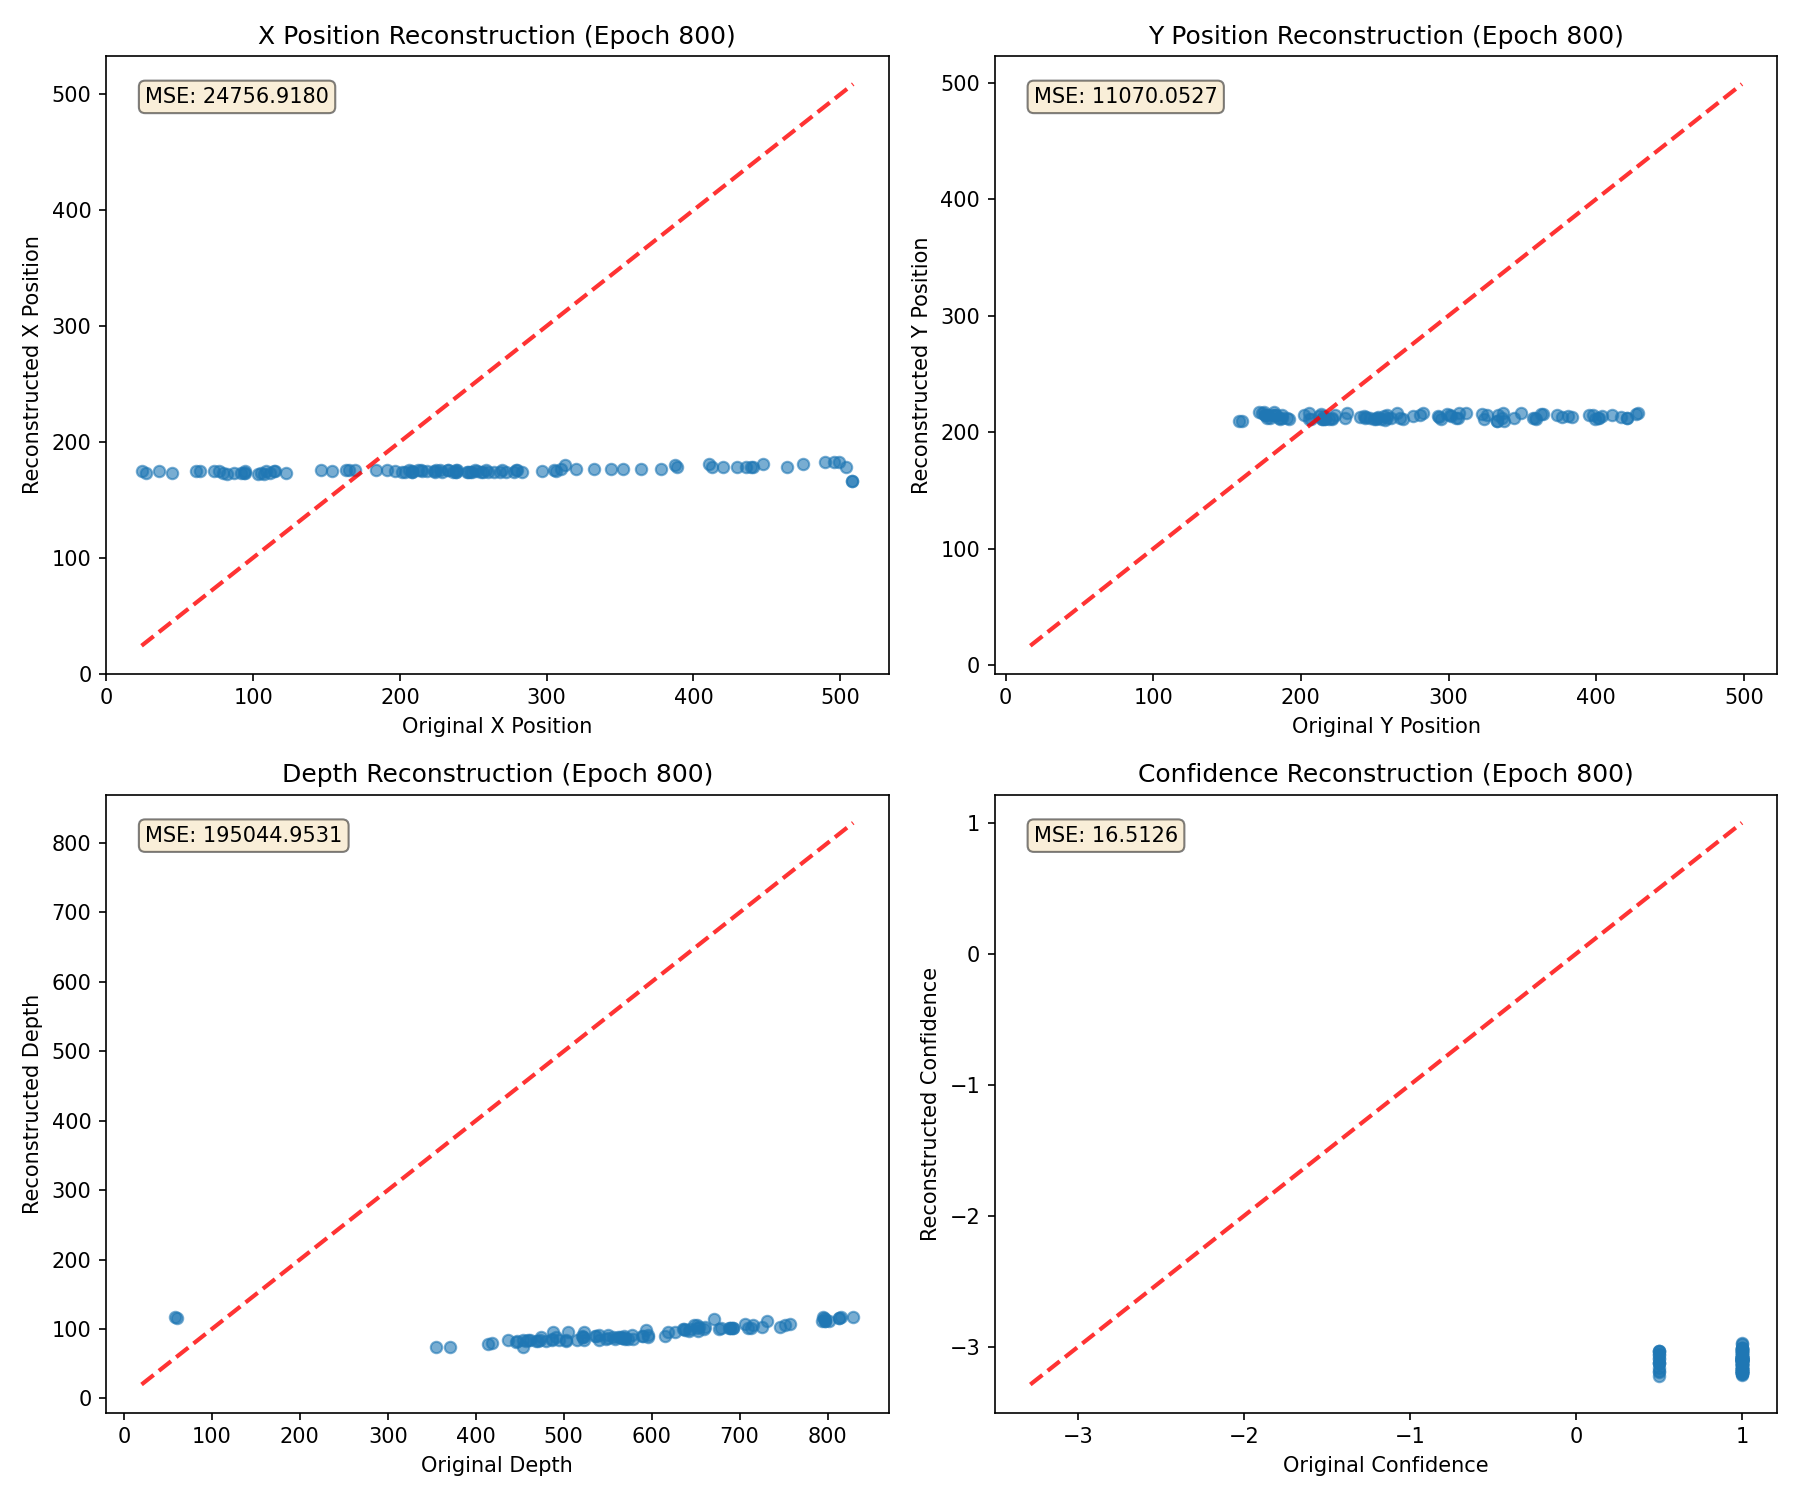
\includegraphics[width=0.4\linewidth]{figures/training_attempt_2/reconstruction_epoch_800.png}
	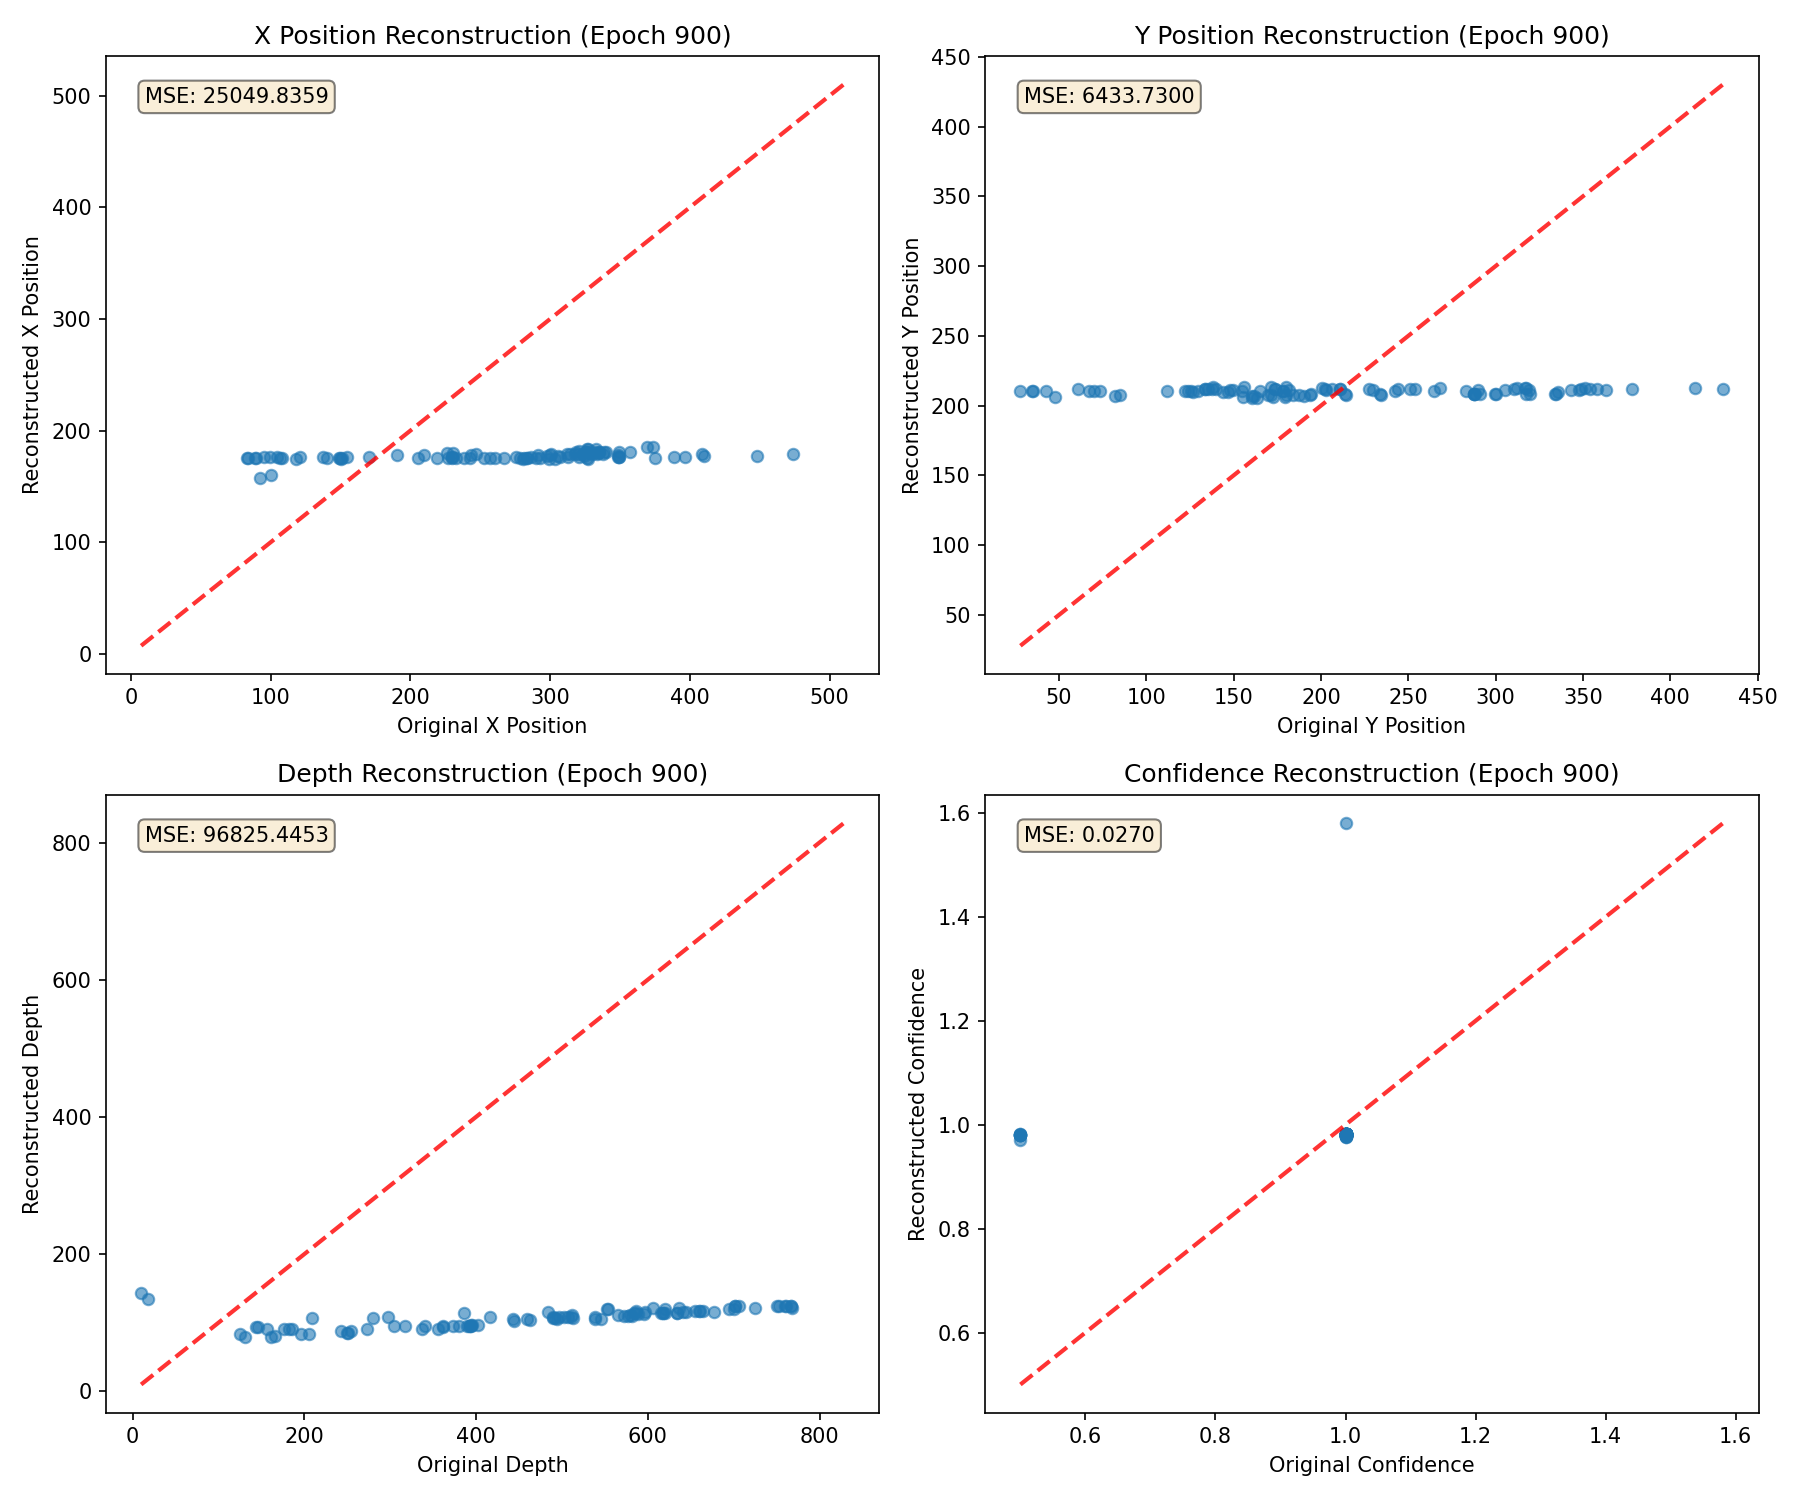
\includegraphics[width=0.4\linewidth]{figures/training_attempt_2/reconstruction_epoch_900.png}
	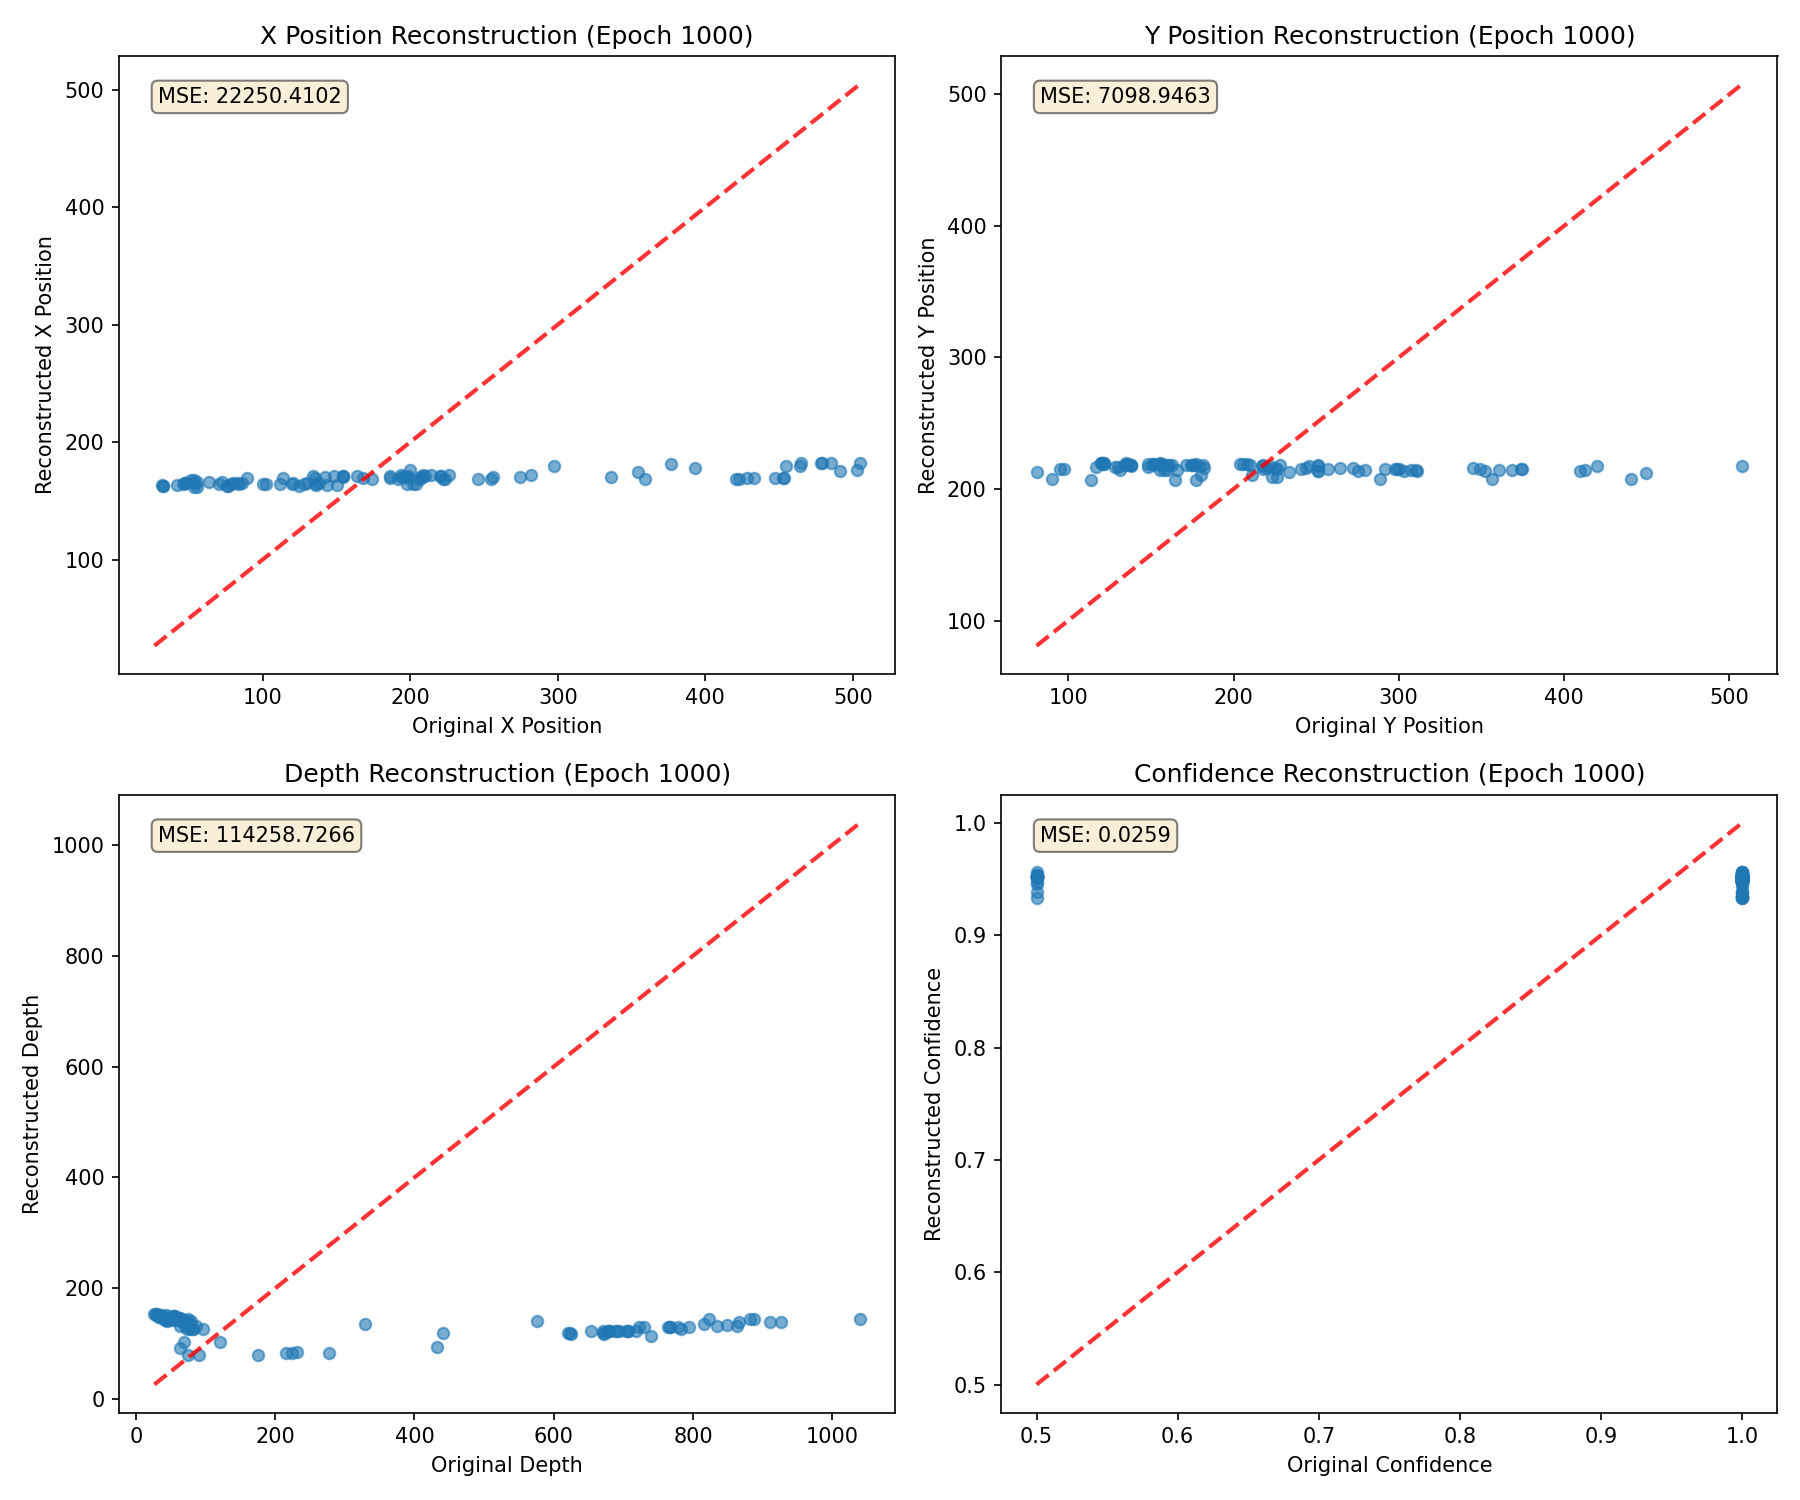
\includegraphics[width=0.4\linewidth]{figures/training_attempt_2/reconstruction_epoch_1000.png}
	\caption{Training with full set and 1500 epochs reconstruction part 2}
	\label{fig:training_attempt_2_reconstruction_epocs_part_2}
\end{figure}


\begin{figure}[H]
	\centering
	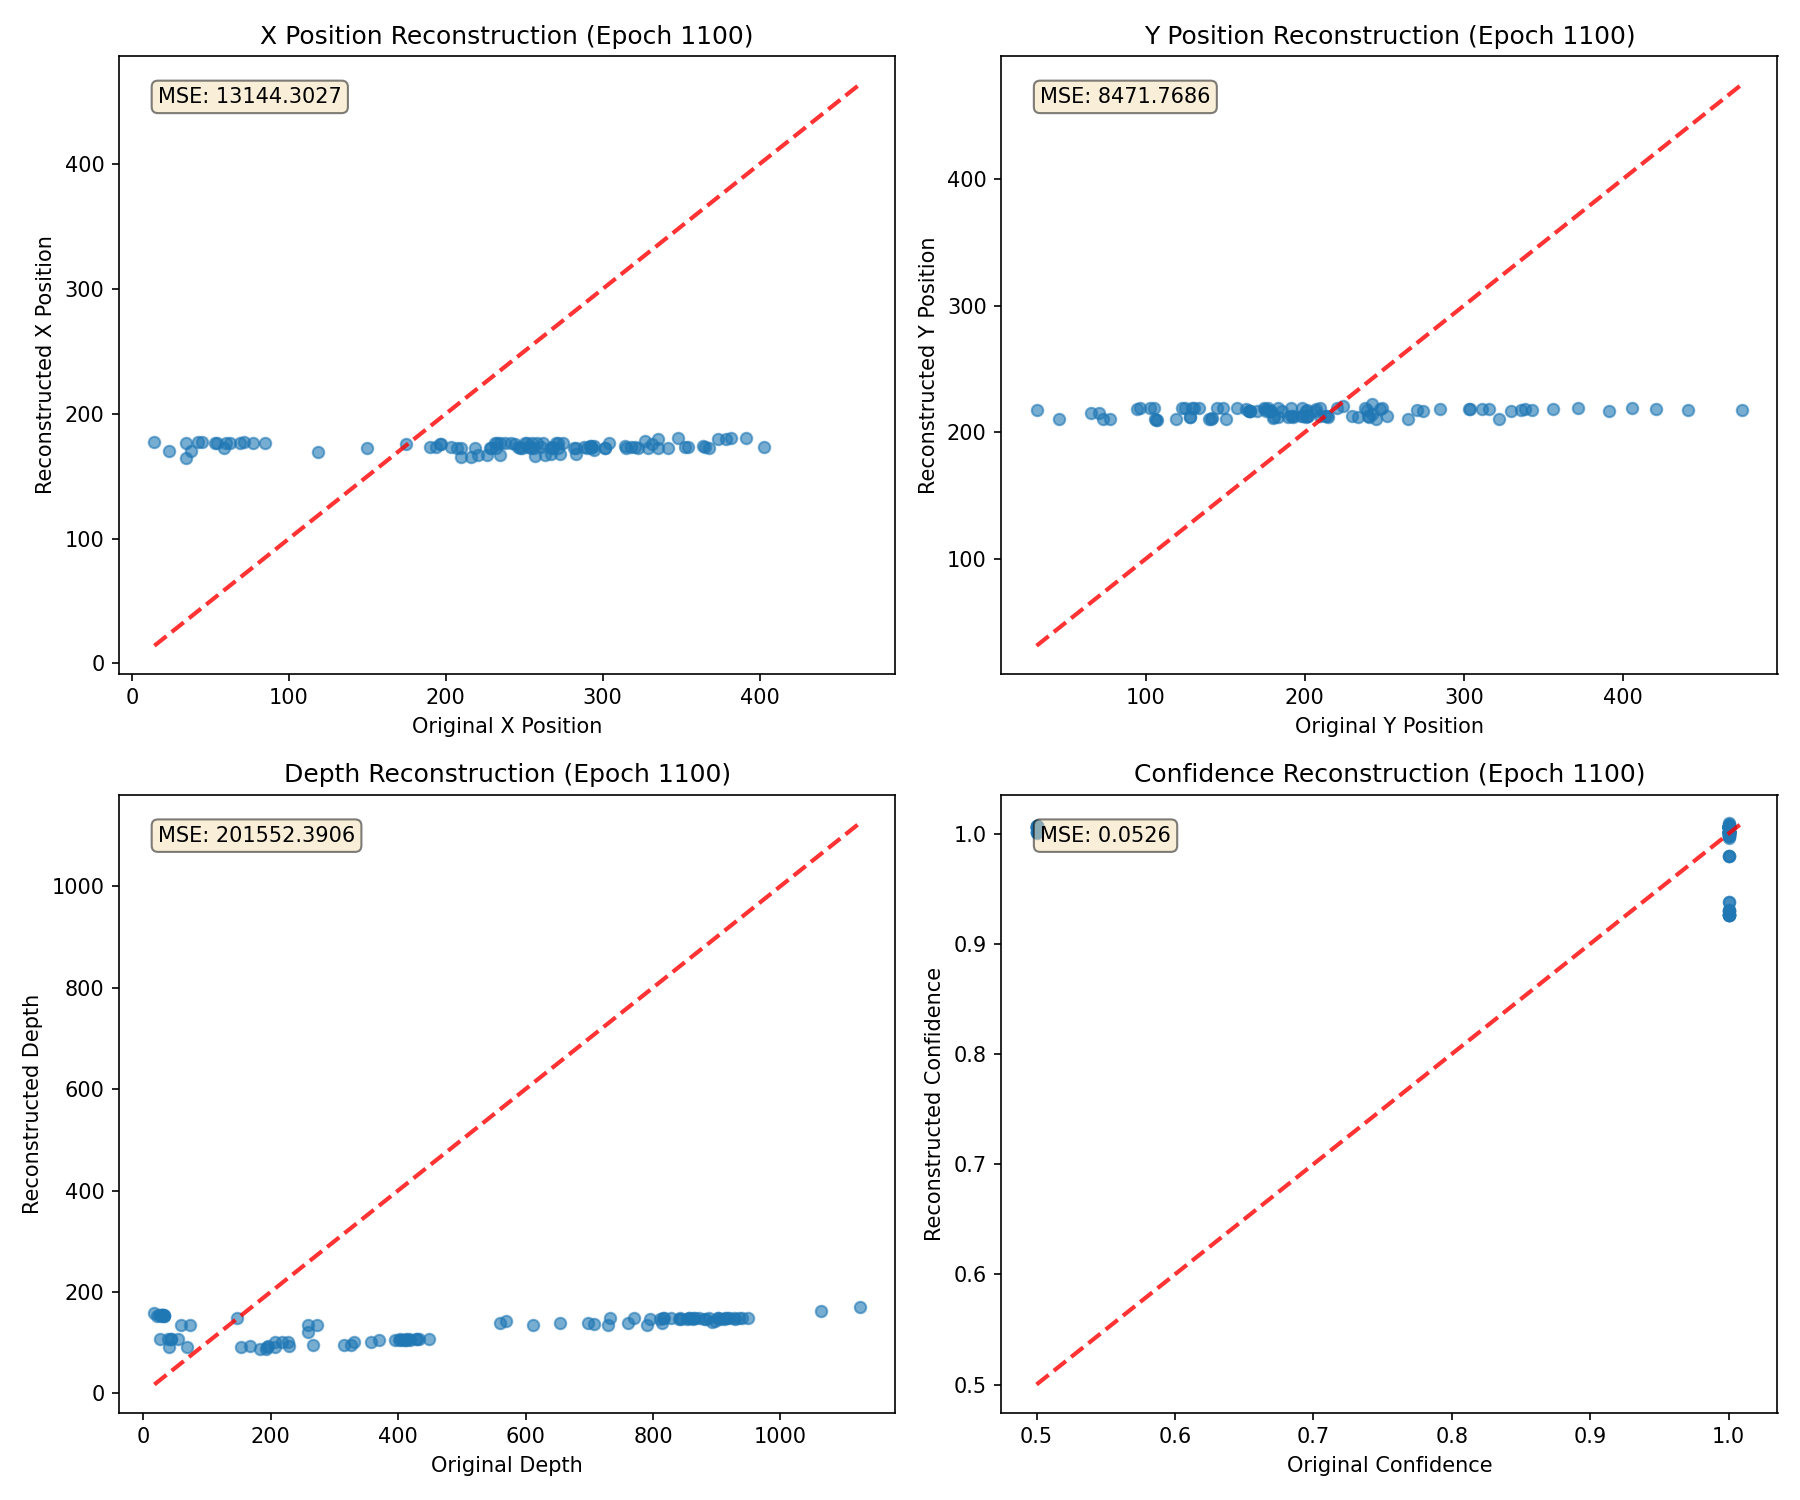
\includegraphics[width=0.4\linewidth]{figures/training_attempt_2/reconstruction_epoch_1100.png}
	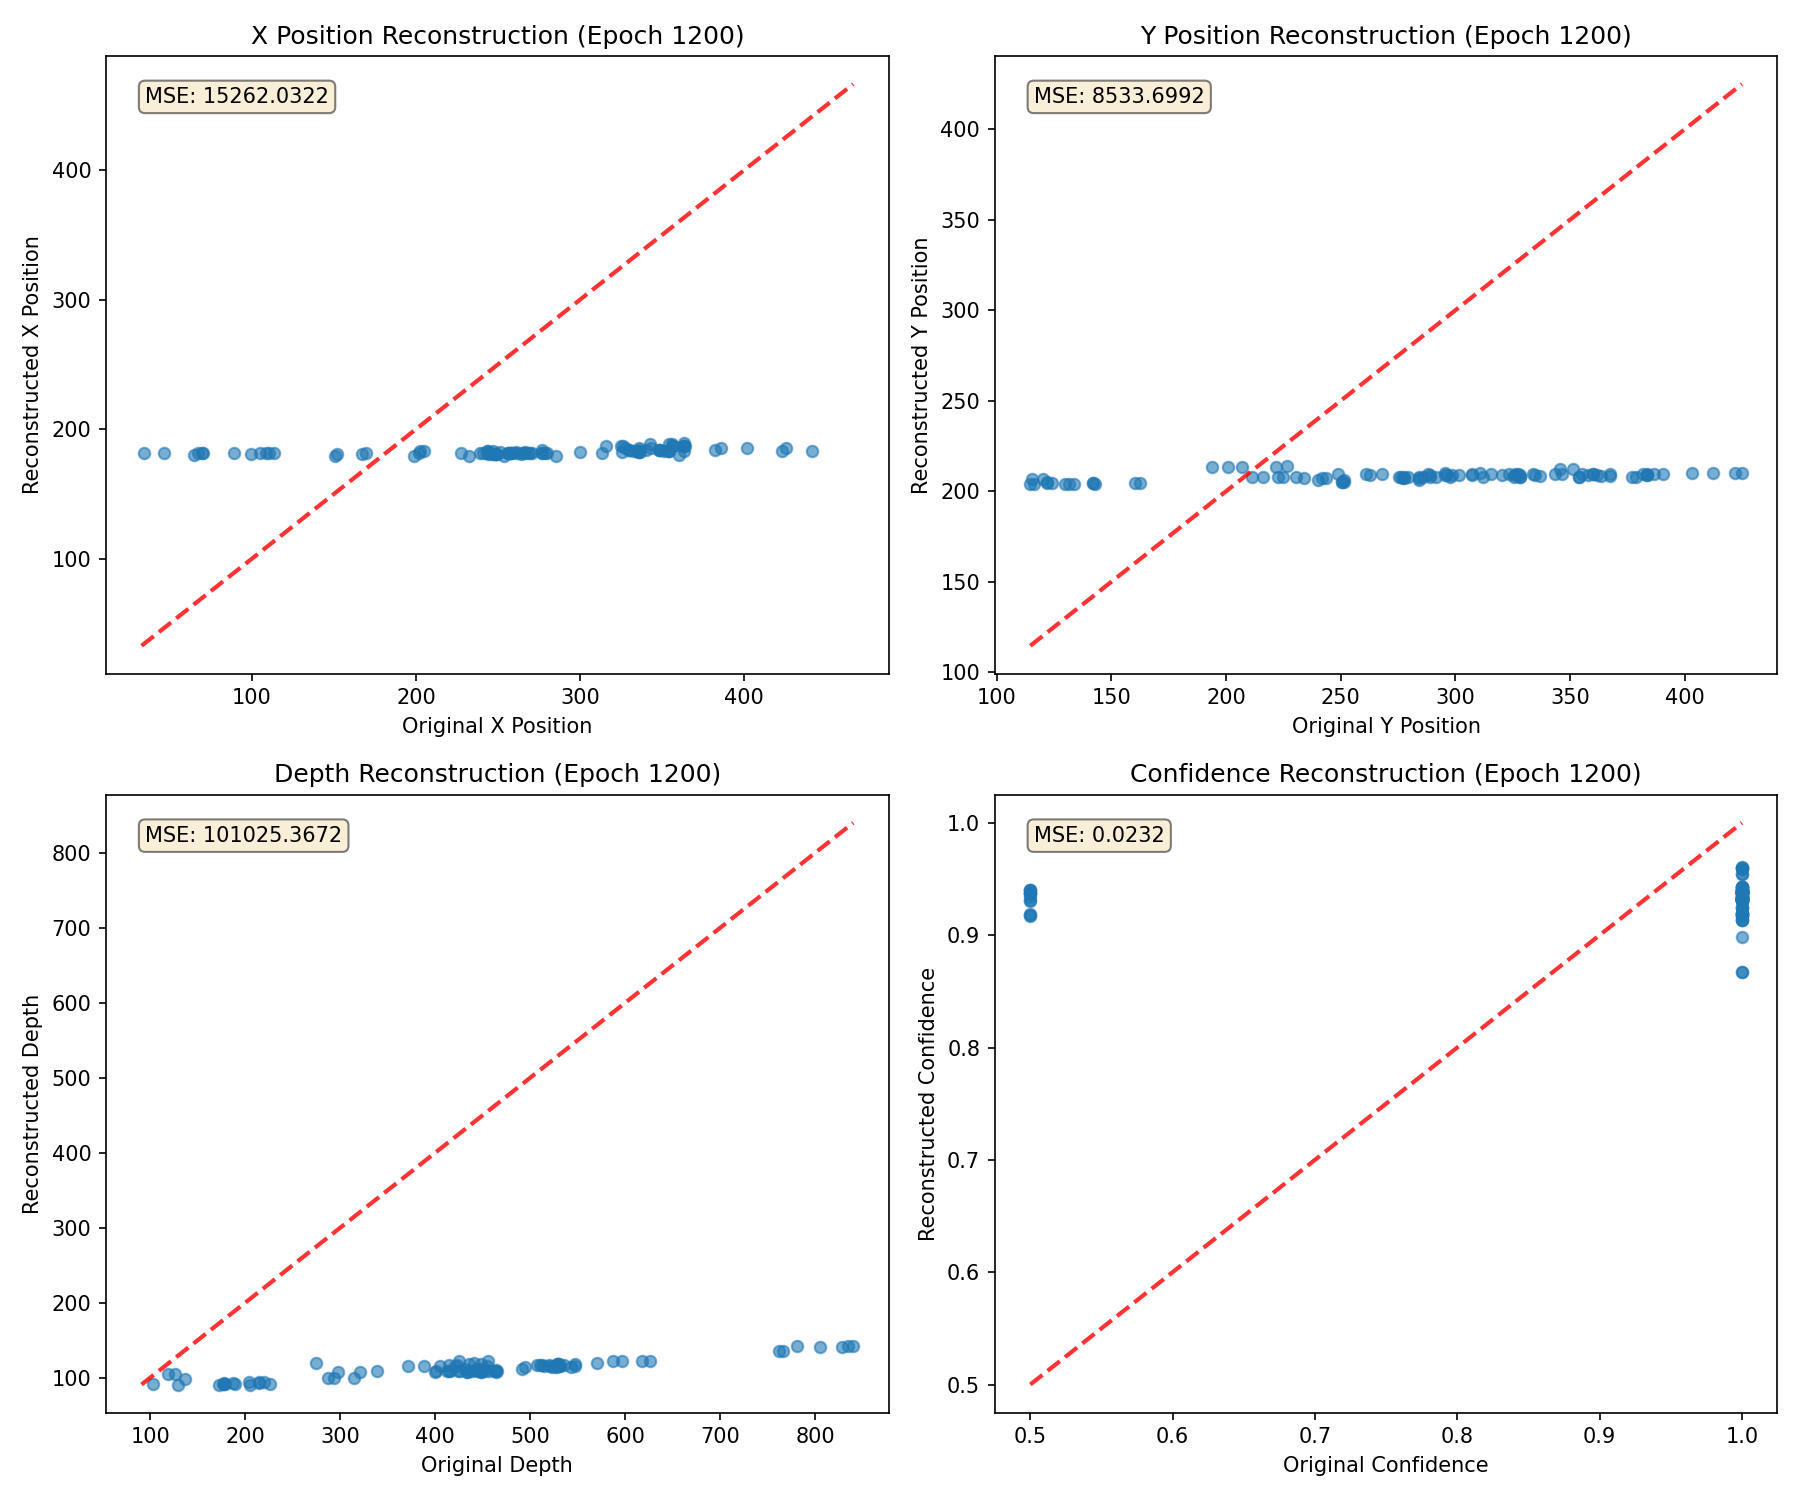
\includegraphics[width=0.4\linewidth]{figures/training_attempt_2/reconstruction_epoch_1200.png}
	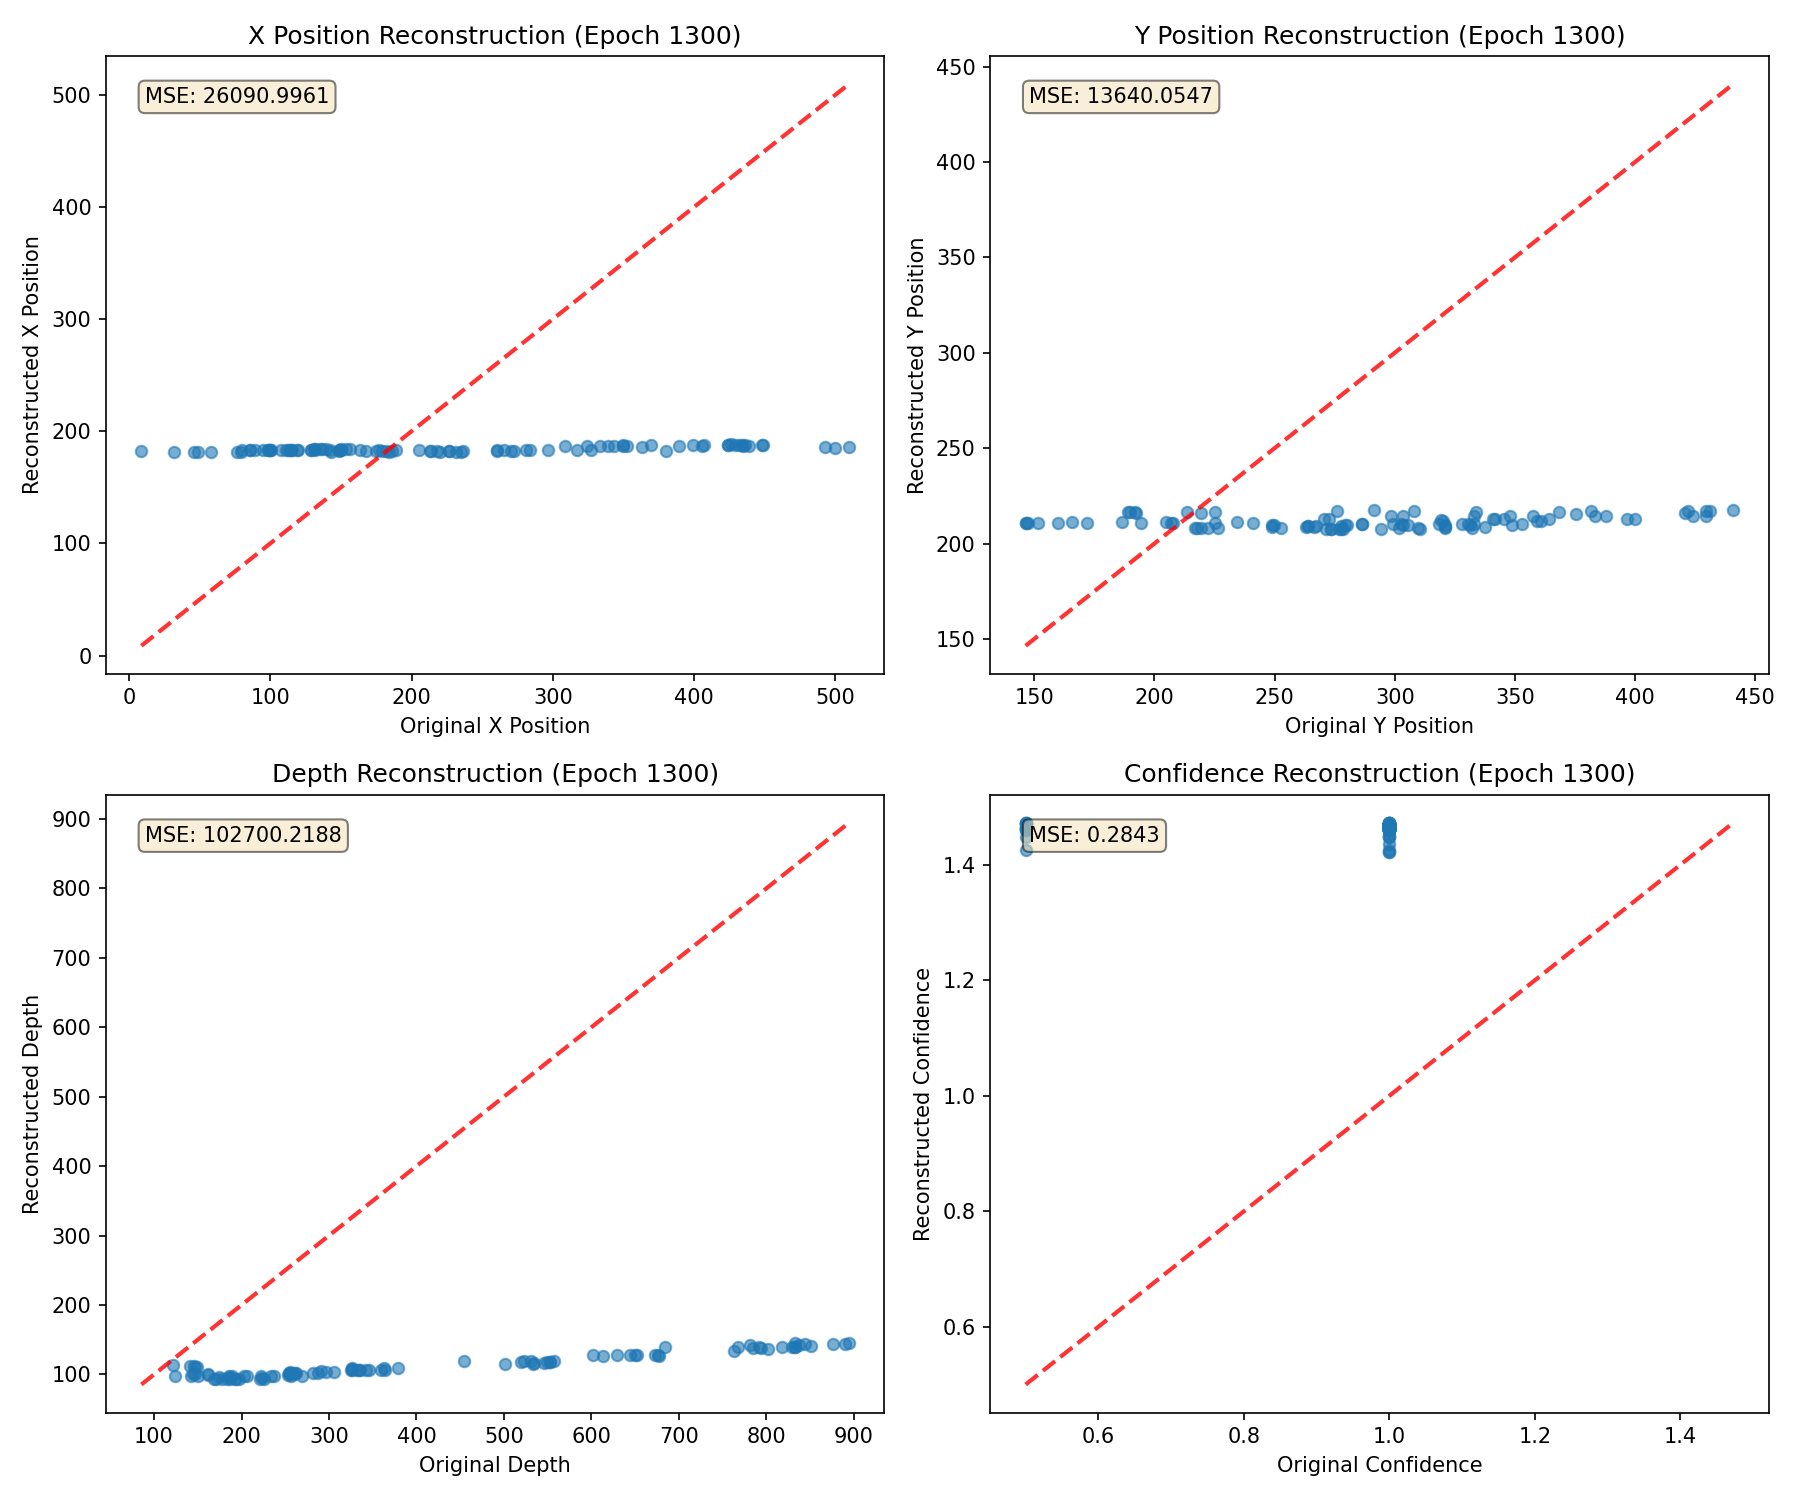
\includegraphics[width=0.4\linewidth]{figures/training_attempt_2/reconstruction_epoch_1300.png}
	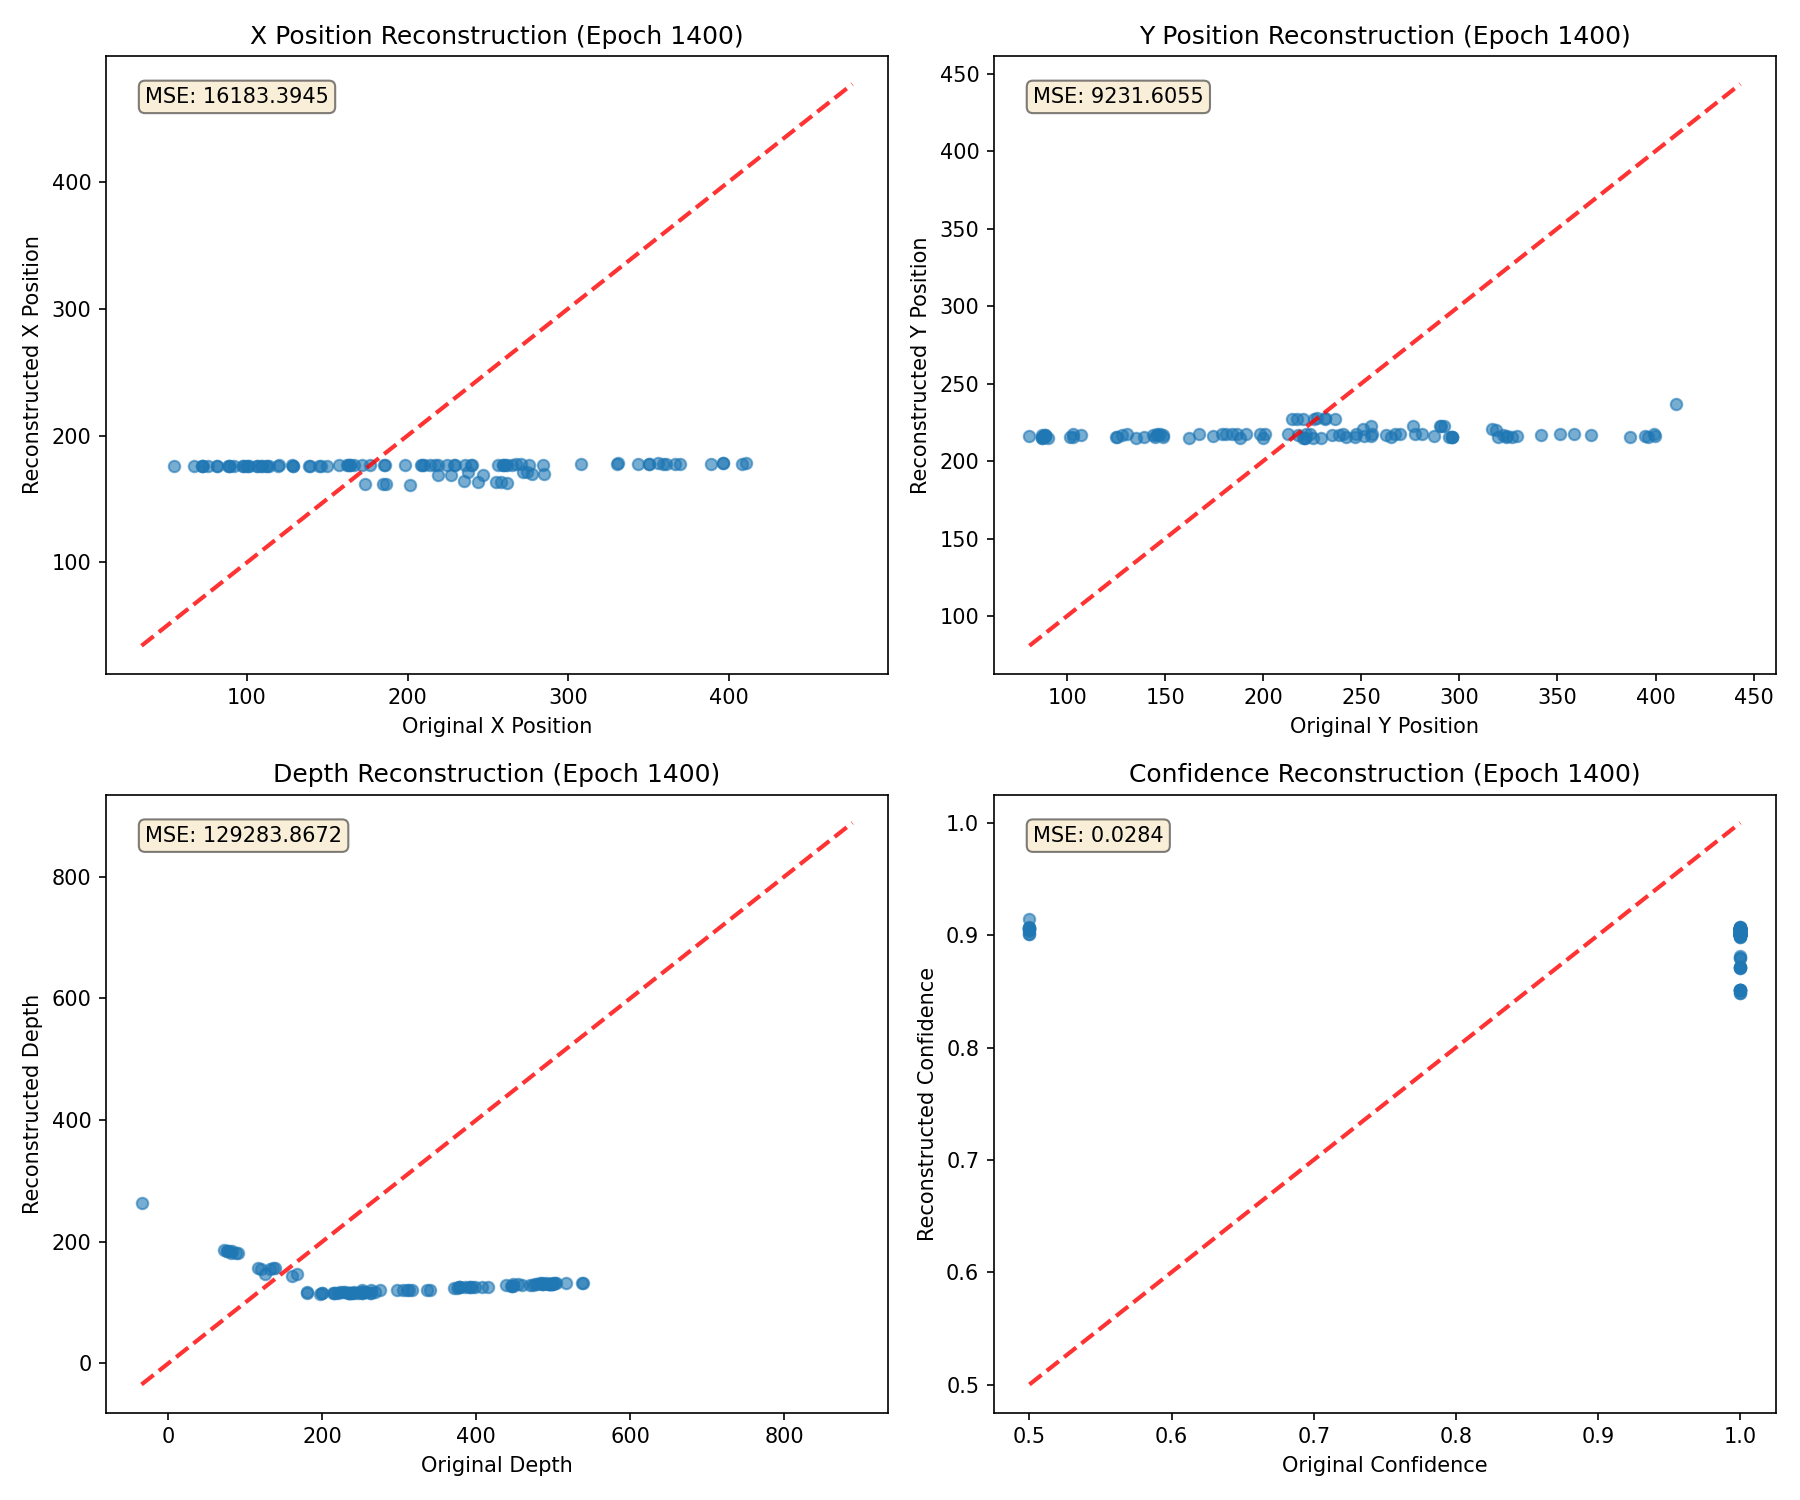
\includegraphics[width=0.4\linewidth]{figures/training_attempt_2/reconstruction_epoch_1400.png}
	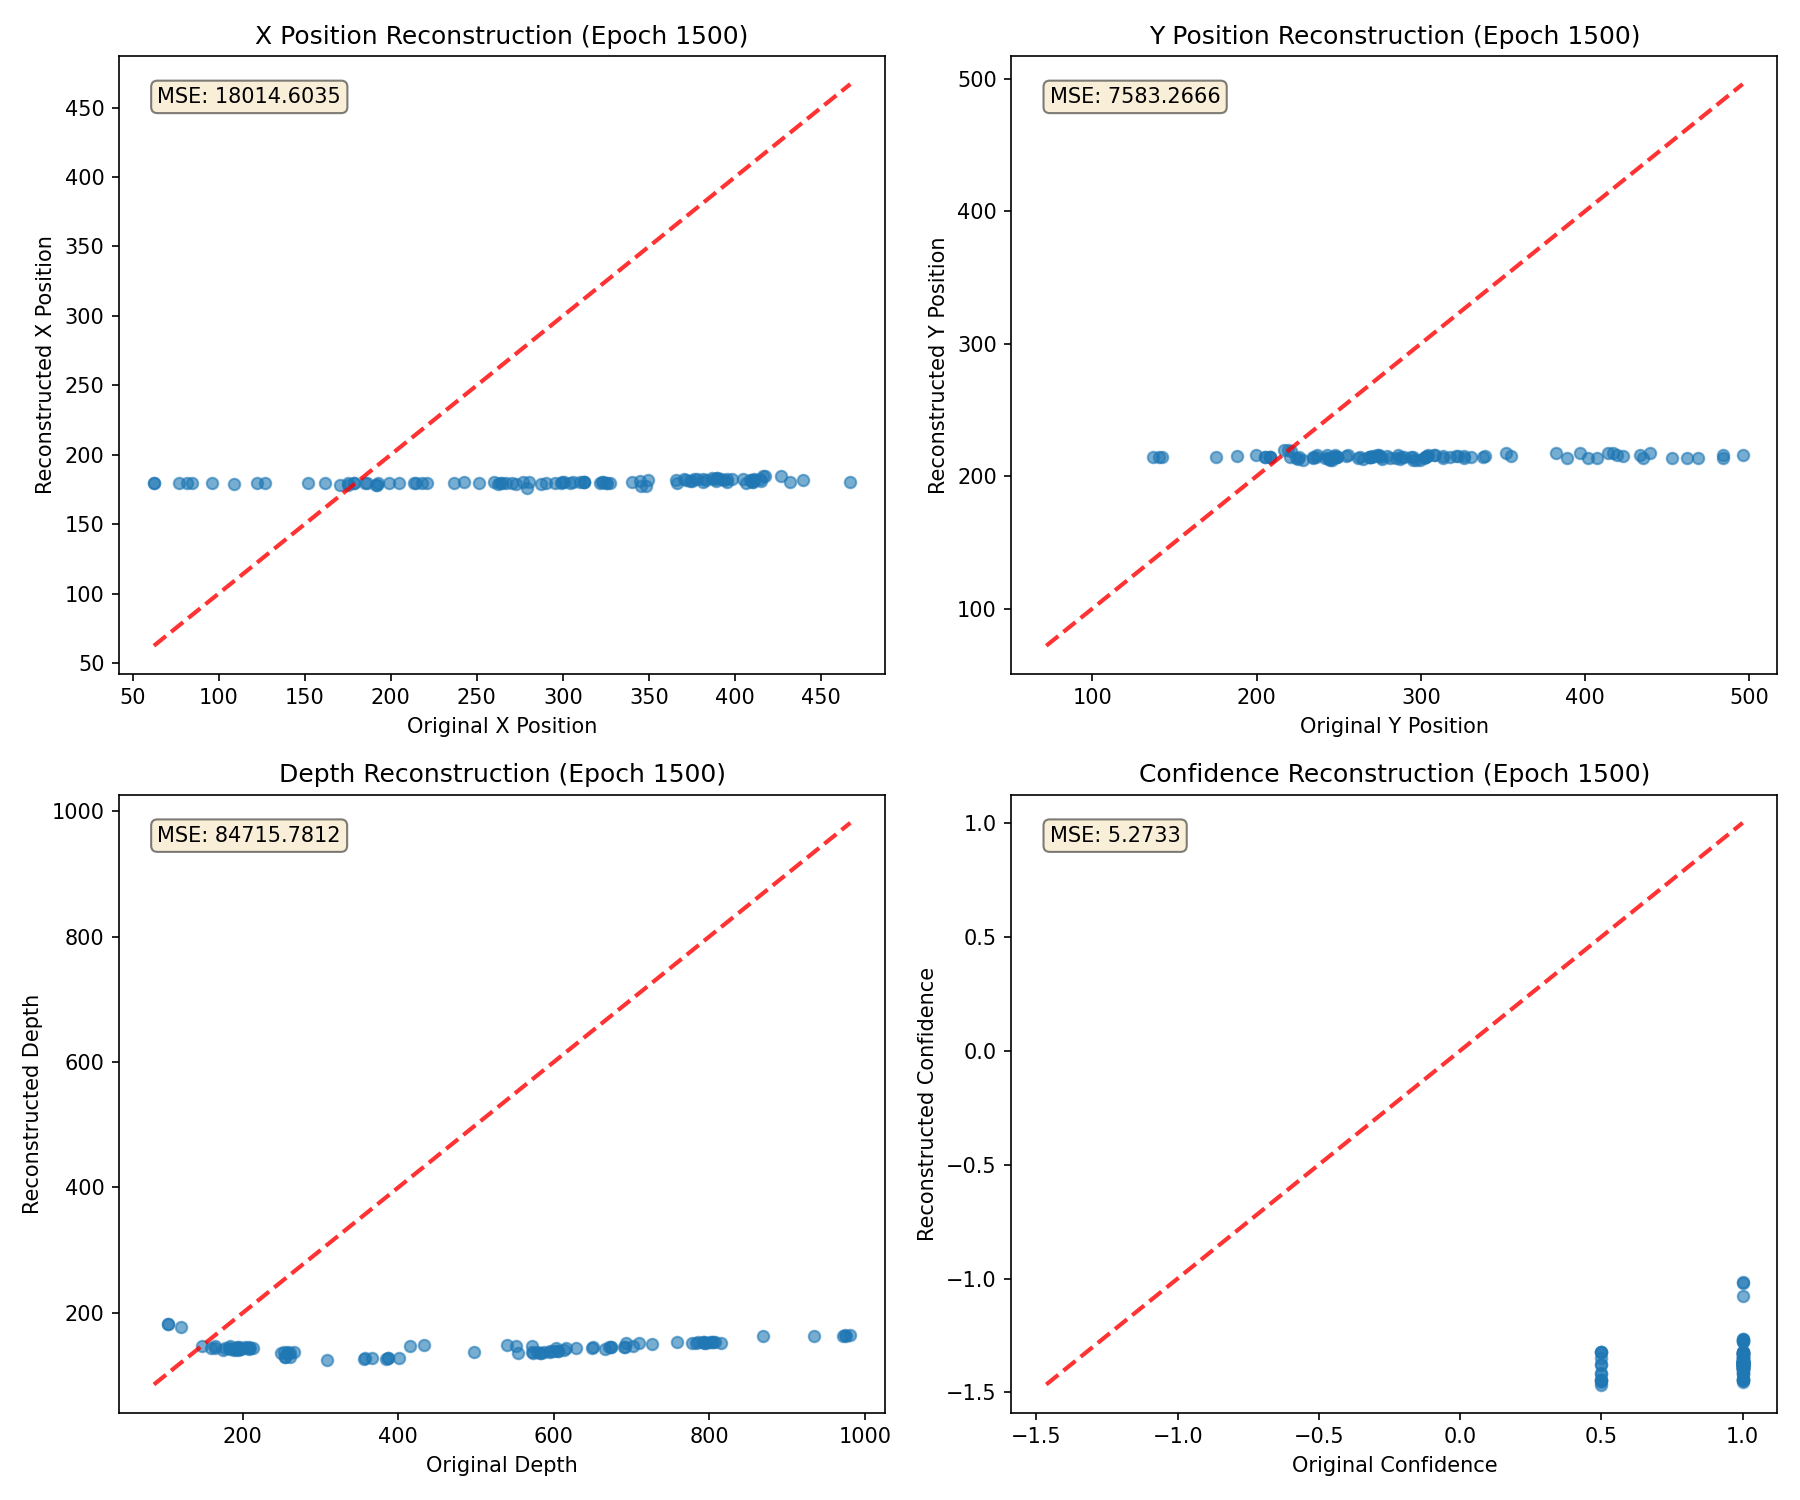
\includegraphics[width=0.4\linewidth]{figures/training_attempt_2/reconstruction_epoch_1500.png}
	\caption{Training with full set and 1500 epochs reconstruction part 3}
	\label{fig:training_attempt_2_reconstruction_epocs_part_3}
\end{figure}

While I'm quite happy that the "training" completed without any errors this is obviously not working at all.
This is definitely not the approach to take.  The GAT is trying to reconstruct the input features [x,y,depth,confidence, <embedding>]
which doesn't really help in learning to group persons by their joint types. Doing this would have allowed the model to learn
to reconstruct the input features but not to learn the relationships between the joint types and the keypoints.

While this isn't exactly the wrong approach (could have been useful for doing both pose estimation and tracking)
it didn't work for some reason. This could just be because the model is not complex enough or something to do with the
hyperparameters. I'm going to assume the model was not complex enough. It's best to try stick to just tracking.

The processing also created seperate graphs for each person which is fine for estimation but not tracking (at least multiperson tracking).

The plotting of reconstruction (which didn't work again because of some reason - hopefully the model) showed how this didn't
work. The reconstruction basically never worked.